\documentclass[12pt,a4paper]{article}
\usepackage[utf8]{inputenc}

\usepackage{amsmath}
\usepackage{amsfonts}
\usepackage{amssymb}
\usepackage{graphicx}
\usepackage{listings}
\usepackage[margin=1.0in]{geometry}
\usepackage{caption}
\usepackage{subcaption}
\usepackage{float}
\usepackage[utf8]{inputenc}
\usepackage{refstyle}
\usepackage{spverbatim}
\usepackage{listings}
\usepackage{csvsimple}
\usepackage{adjustbox}
\usepackage{cancel}
\usepackage{scalerel,stackengine}
\stackMath
\newcommand\reallywidehat[1]{%
\savestack{\tmpbox}{\stretchto{%
  \scaleto{%
    \scalerel*[\widthof{\ensuremath{#1}}]{\kern-.6pt\bigwedge\kern-.6pt}%
    {\rule[-\textheight/2]{1ex}{\textheight}}%WIDTH-LIMITED BIG WEDGE
  }{\textheight}% 
}{0.5ex}}%
\stackon[1pt]{#1}{\tmpbox}%
}
\parskip 1ex

\lstset{numbers=left,
	title=\lstname,
	numberstyle=\tiny, 
	breaklines=true,
	tabsize=4,
	language=Python,
	morekeywords={with,super,as},,
	frame=single,
	basicstyle=\footnotesize\tt,
	commentstyle=\color{comment},
	keywordstyle=\color{keyword},
	stringstyle=\color{string},
	backgroundcolor=\color{background},
	showstringspaces=false,
	numbers=left,
	numbersep=5pt,
	literate=
		{æ}{{\ae}}1
		{å}{{\aa}}1
		{ø}{{\o}}1
		{Æ}{{\AE}}1
		{Å}{{\AA}}1
		{Ø}{{\O}}1
	}

\usepackage{bm}
\usepackage{hyperref}
\usepackage[usenames, dvipsnames]{color}

\begin{document}

\begin{center}
\LARGE{\textbf{Project 1: Classification and Regression, from linear and logistic regression to neural networks}}
\\
\large{\textbf{Course: FYS-STK4155}}
\\
\large{\textbf{Semester: Autumn 2020}}
\\
\large{\textbf{Name: Sander Losnedahl}}
\end{center}

\begin{center}
\Large{\textbf{Abstract}}
\end{center}

\noindent a

\newpage

\begin{center}
\Large{\textbf{Introduction}}
\end{center}

\noindent This project aims to implement a neural network algorithm that can train both regression and classification models. The resulting test errors from the two types of models will then be compared to the results from a linear regression scheme and a logistic regression scheme. 
\\
We start with the former by implementing a stochastic gradient descent (SGD) algorithm where the goal is the predict the Franke function. This function is a weighted sum of exponentials and the evaluation of the prediction will be both in terms of MSE and $R^2$. Then, a neural network is implemented with a varying number of hidden neurons/layers utilizing multiple hidden layer activation functions and a stochastic gradient descent when tuning the weights in the backpropagation. The results from the final and most optimized model is then compared to the results from the SGD model and the differences are made clear.
\\
We then move on to classification where we can utilize the same neural network algorithm, but changing the activation function in the output layer to the softmax function which yields a probability distribution. The model is then trained on images of hand-written digits and a prediction is made based on the training probability distribution. The evaluation of the algorithm will be in terms of the accuracy scores which simply measures the rate of successfully predicted images. The final and most optimized model is then compared to a logistic regression in the form of a logistic SGD algorithm. The results are compared and the pros and cons of each approach is highlighted.
\\
Finally, the results are summarized and conclusions are drawn based on the results of the described algorithms. Then, future improvements upon the implemented algorithms are discussed.

\newpage

\begin{center}
\Large{\textbf{Preliminaries}}
\end{center}

\noindent \textbf{The github page} can be found at \href{{https://github.com/sanderwl/FYS-STK4155/tree/master/Project2/Project2}}{\nolinkurl{https://github.com/sanderwl/FYS-STK4155/tree/master/Project2/Project2}} under the folder "project 2". This is where you find all the implemented code and results in this project.
\\
\textbf{Scaling the data} was a necessity to make the algorithms work. The scaling in this project was done by subtracting the mean and dividing by the standard deviation of the data. This makes the data zero-centred with a standard deviation of one. Doing this will increase the predictive capabilities of the algorithms and make the results more interpretable.

\newpage

\begin{center}
\Large{\textbf{Exercise 1a): Stochastic gradient descent}}
\end{center}

\begin{center}
\large{\textbf{The Franke function}}
\end{center}

\noindent In this first part of the exercise, we focus on regression by training a neural network to predict the Franke function. The Franke function is a weighted sum of exponentials given by equation \ref{eq:Franke}

\begin{equation}\label{eq:Franke}
\begin{aligned}
f(x,y) &= \frac{3}{4}\exp{\left(-\frac{(9x-2)^2}{4} - \frac{(9y-2)^2}{4}\right)}+\frac{3}{4}\exp{\left(-\frac{(9x+1)^2}{49}- \frac{(9y+1)}{10}\right)} \\
&+\frac{1}{2}\exp{\left(-\frac{(9x-7)^2}{4} - \frac{(9y-3)^2}{4}\right)} -\frac{1}{5}\exp{\left(-(9x-4)^2 - (9y-7)^2\right) }
\end{aligned}
\end{equation}

\noindent where x and y are in the span of 0 and 1. The Franke function will be fit using polynomials of up to degree 5, as this was proven yield the best fit in Project one (the report can be found at \href{{https://github.com/sanderwl/FYS-STK4155/tree/master/Project1/Report}}{\nolinkurl{https://github.com/sanderwl/FYS-STK4155/tree/master/Project1/Report}}). The number of observations is set to 100 as this was also applied in the Project one. Keeping the consistency will make for better comparison later in this Project. The Franke function can be plotted and is shown i figure \ref{fig:Franke}

\begin{figure}[H]
\centering
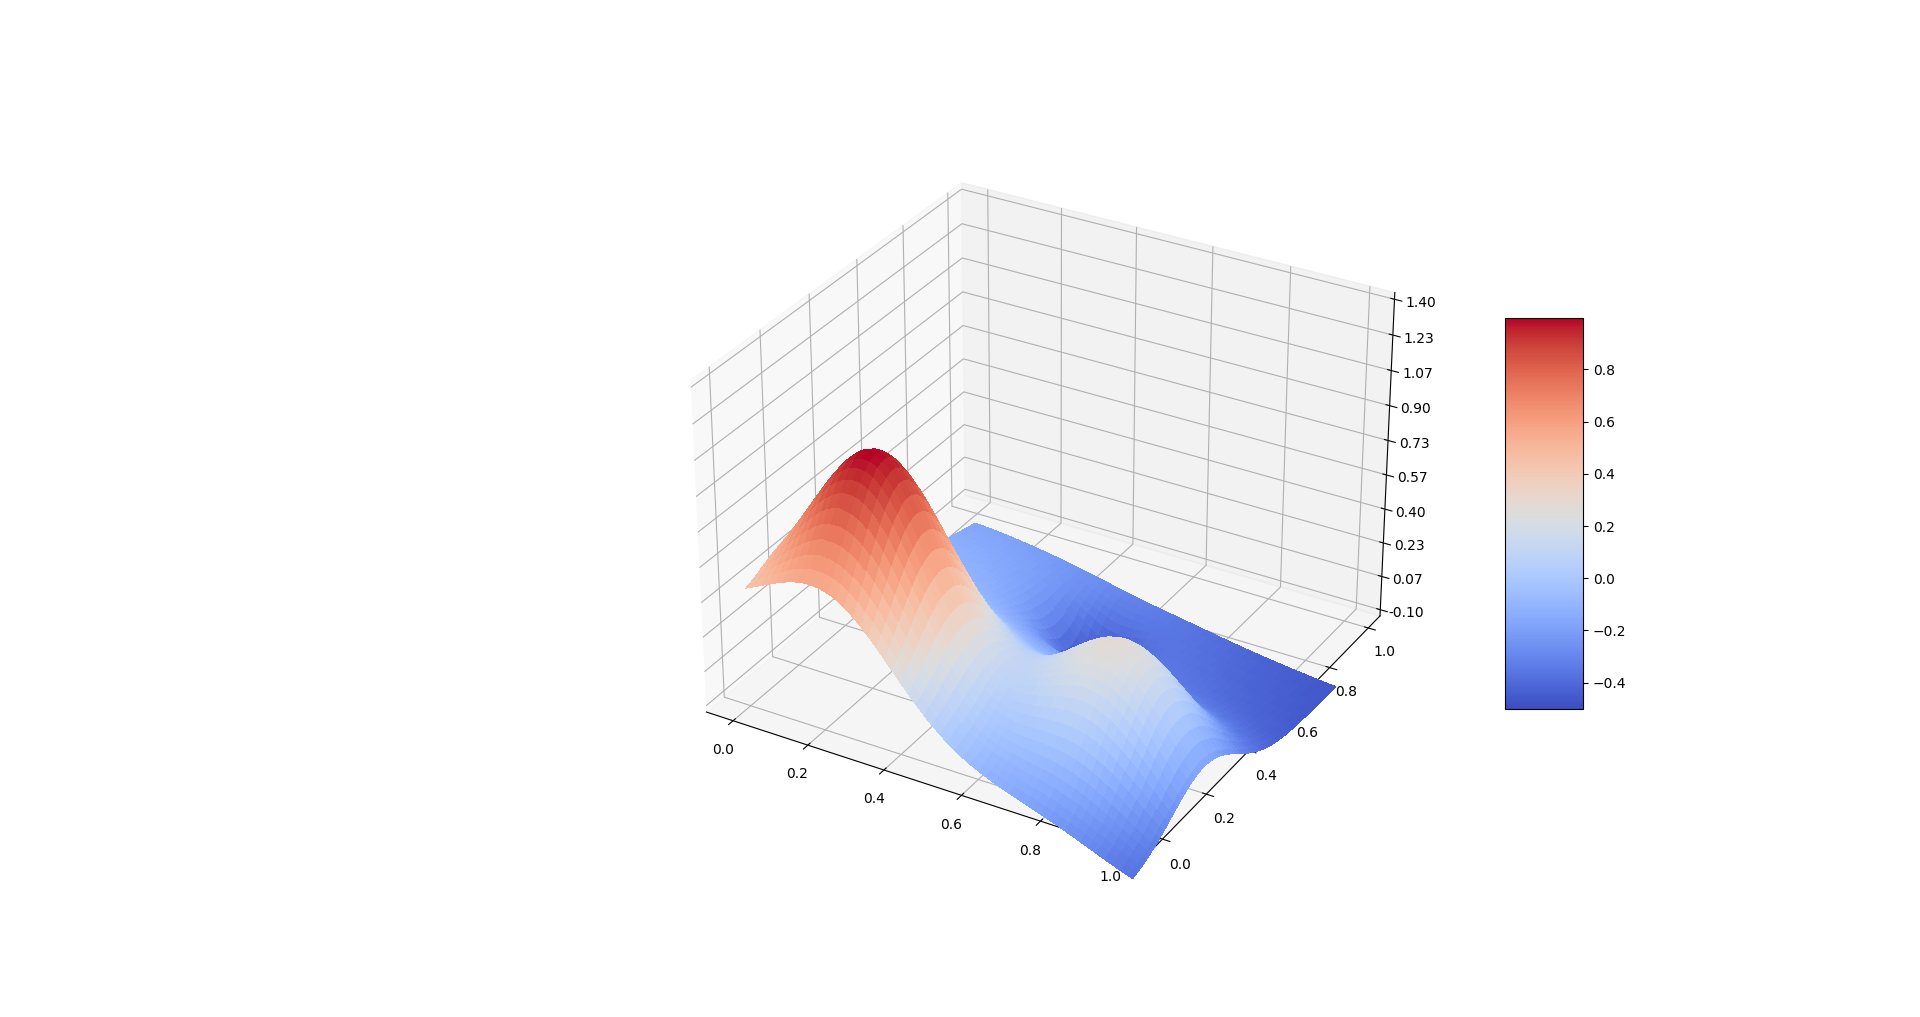
\includegraphics[width = 1\linewidth]{C:/Users/Sander/Documents/GitHub/FYS-STK4155/Project2/Project2/Report/Figures/FrankOG.PNG}
\caption{\label{fig:Franke} A plot of the Franke function discretized with 100 times a 100 observations. The function is standardized and normalized such that the mean is zero and the variance is 1 and the maximum value is 1.}
\end{figure}

\begin{center}
\large{\textbf{Concepts of gradient descent and the cost function}}
\end{center}

\noindent In the last project, we utilized least squares solutions on the form $\boldsymbol{\hat{\beta}} = (\textbf{X}^T\textbf{X})^{-1}\textbf{X}^T\hat{y}$ in order to find the regression coefficients yielding the lowest residual sum of squares. However, this method relies on taking an matrix inverse of the data, which often is not feasible. Another approach which does not utilize matrix inversion is gradient descent. This method instead relies on finding the minimum value of some cost function dependent on the regression coefficients. In this exercise, we will use the MSE as the cost function is given by equation \ref{eq:MSEdef}

\begin{equation}\label{eq:MSEdef}
\begin{aligned}
MSE = C(\boldsymbol{\beta}) = \frac{1}{n}\sum_{i = 1}^n (f - \hat{y})^2
\end{aligned}
\end{equation}

\noindent where f is the Franke function we are trying to predict and $\hat{y}$ is the prediction. Like previously mentioned, we want to find where this function has its minimum, as this point will yield the best regression coefficients. Gradient descent does not attempt to find this point directly, but iteratively. We can find the gradient of equation \ref{eq:MSEdef} and iteratively move the values of our regression coefficients along the line of most negative gradient. After a given number of iterations, we are bound to find the minimum of the cost function, or at least a local minimum (this will be discussed later). In order to find the gradient, we can simply take the partial derivative of equation \ref{eq:MSEdef} with respect to each individual regression coefficient

\begin{equation}\label{eq:MSEder}
\begin{aligned}
\frac{\partial C(\boldsymbol{\beta})}{\partial \boldsymbol{\beta}} 
\\
\frac{\partial \frac{1}{n} \sum_{i = 1}^n (f-\hat{y})^2}{\partial \boldsymbol{\beta}} 
\\
\frac{\partial \frac{1}{n} \sum_{i = 1}^n (f-\textbf{X}\boldsymbol{\hat{\beta}})^2}{\partial \boldsymbol{\beta}} 
\\
\frac{2}{n} \sum_{i = 1}^n \textbf{X}(f - \textbf{X}\boldsymbol{\hat{\beta}}) 
\end{aligned}
\end{equation}

\noindent As mentioned, we iteratively follow the direction in which the gradient is most negative. The number of iterations to perform is called the epoch and is usually just set to a very high number. When we are approaching the minimum or a local minimum, the algorithm which only follows the gradient will be "stuck" and wiggle back and fourth around this minimum or local minimum. Therefore, any iterations following the point of becoming "stuck" is useless, so the algorithm should be stopped at this point.
\\
We have so far only discussed in which direction we are to move, but how large steps should we take in that direction? This parameter is called the learning rate and is typically in the between zero and one (around $0.01$). The learning parameter can either be static or adaptive. The former means that we are only moving a set distance every iteration, while the latter means that we are changing the distance we are moving depending on what iterations we are currently on. A adaptive learning rate depends on the schedule which sets the learning rate for each epoch iteration. In this project we use the time based schedule which is given by equation \ref{eq:scheduleTIME}

\begin{equation}\label{eq:scheduleTIME}
\begin{aligned}
\frac{t_0}{t + t_1}
\end{aligned}
\end{equation}

\noindent where $t_0$ and $t_1$ are constants and t is given by epoch iterations $\times$ number of samples. 
\\
The problem with gradient descent is that if we have a very large number of features (polynomial degrees here), the gradient descent algorithm will take a very long time to run. To counter this problem, we introduce a variant of the gradient descent called stochastic gradient descent.

\begin{center}
\large{\textbf{Taking a stochastic approach to gradient descent}}
\end{center}

\noindent The stochastic gradient descent approach relies on simply utilizing a part of the entire data. The part used is called batch or mini-batch and can be just a single observation (actual stochastic gradient descent) or some where in between one and the number of observations (semi-stochastic gradient descent). This technique works as we are iterating over the number of batches as well as the number of epochs, each time taking a random sample from the original observations. Taking only a sample from the observation works because we are repeating the gradient descent process a large number of times equal to $\frac{\textrm{number of observations}}{\textrm{size of batch}}$. Since we are only utilizing one or a few number of observations, equation \ref{eq:MSEder} can be written as

\begin{equation}\label{eq:MSEderSTO}
\begin{aligned}
2 \textbf{X}(f - \textbf{X}\boldsymbol{\hat{\beta}}) 
\end{aligned}
\end{equation}

\noindent and the t in equation \ref{eq:scheduleTIME} will instead be epoch iteration $\times$ number of samples $+$ batch iteration.
\\
So far we have only considered the gradient descent in terms of its least squares equivalent, however, we also want to implement the ridge equivalent. In the Ridge case, the gradient descent concept and algorithm is exactly the same as the OLS case, but the gradient at which we try to find the MSE minimum look slightly different as we need to add a penalty term $\lambda \times \boldsymbol{\hat{\beta}}$ as shown in equation \ref{eq:MSEderSTOridge}

\begin{equation}\label{eq:MSEderSTOridge}
\begin{aligned}
2 \textbf{X}(f - \textbf{X}\boldsymbol{\hat{\beta}}) + \lambda \boldsymbol{\hat{\beta}}
\end{aligned}
\end{equation}

\noindent where the penalty parameter $\lambda$ is typically between zero and one. 

\begin{center}
\large{\textbf{Parameter dependencies for static learning rate}}
\end{center}

\noindent So far we have merely discussed the theoretical concepts of gradient descent, but now we will implement to perform the stochastic gradient descent. We will then vary the different parameters and see how our cost function varies with the different parameters. First, let us set up some standard parameters so we keep the analysis consistent as seen in table \ref{tab:standardParam}

\begin{table}[h]
\caption{\label{tab:standardParam} An overview of standard parameters to be used in the analysis.}
\centering
\begin{tabular}{c|c|c|c|c}
 & static OLS & static Ridge & adaptive OLS & adaptive Ridge\\
\hline
Number of observation n & $100$ & $100$ & $100$ & $100$\\
\hline
Noise-level & $0.001$ & $0.001$ & $0.001$ & $0.001$\\
\hline
Penalty $\lambda$ & None & $0.01$ & None & $0.01$\\
\hline
Model complexity p & $5$ & $5$ & $5$ & $5$\\
\hline
Batch size & $10$ & $10$ & $10$ & $10$\\
\hline
Epoch size & $100$ & $100$ & $100$ & $100$\\
\hline
Initial learning rate & $0.01$ & $0.01$ & $0.01$ & $0.01$\\
\hline
Schedule & None & None & $\frac{t_0}{t+t_1}$ & $\frac{t_0}{t+t_1}$\\
\end{tabular}
\end{table}

\noindent We can now use the values in table \ref{tab:standardParam} as a standard when we want to study the dependence on a single parameter. Let us first study how the MSE varies as function of an increasing number of epoch iterations using our standard parameters with static learning rate

\begin{figure}[H]
\centering
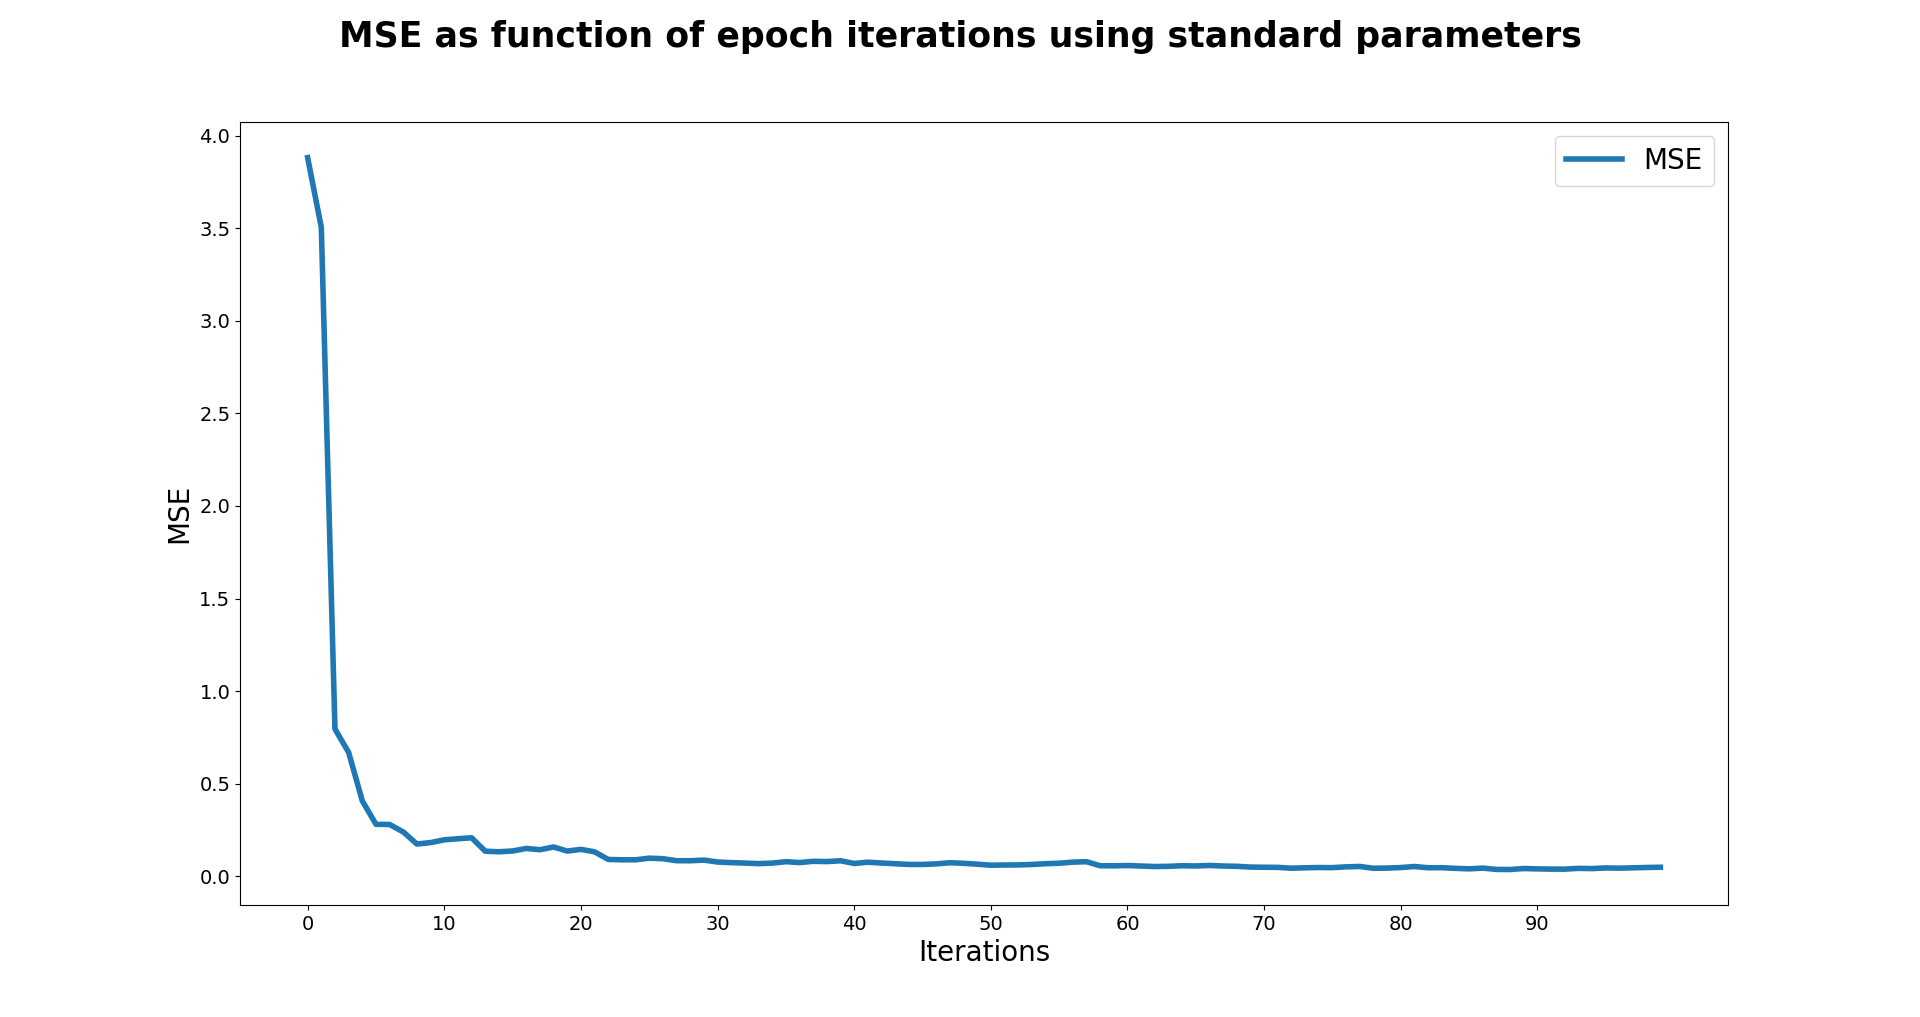
\includegraphics[width = 1\linewidth]{C:/Users/Sander/Documents/GitHub/FYS-STK4155/Project2/Project2/Report/Figures/MSEvsEPOCH_StandardOLS.PNG}
\caption{\label{fig:MSEvsEPOCHstandard} The MSE as function of number of epoch iterations using static learning rate and OLS equivalent SGD.}
\end{figure}

\begin{figure}[H]
\centering
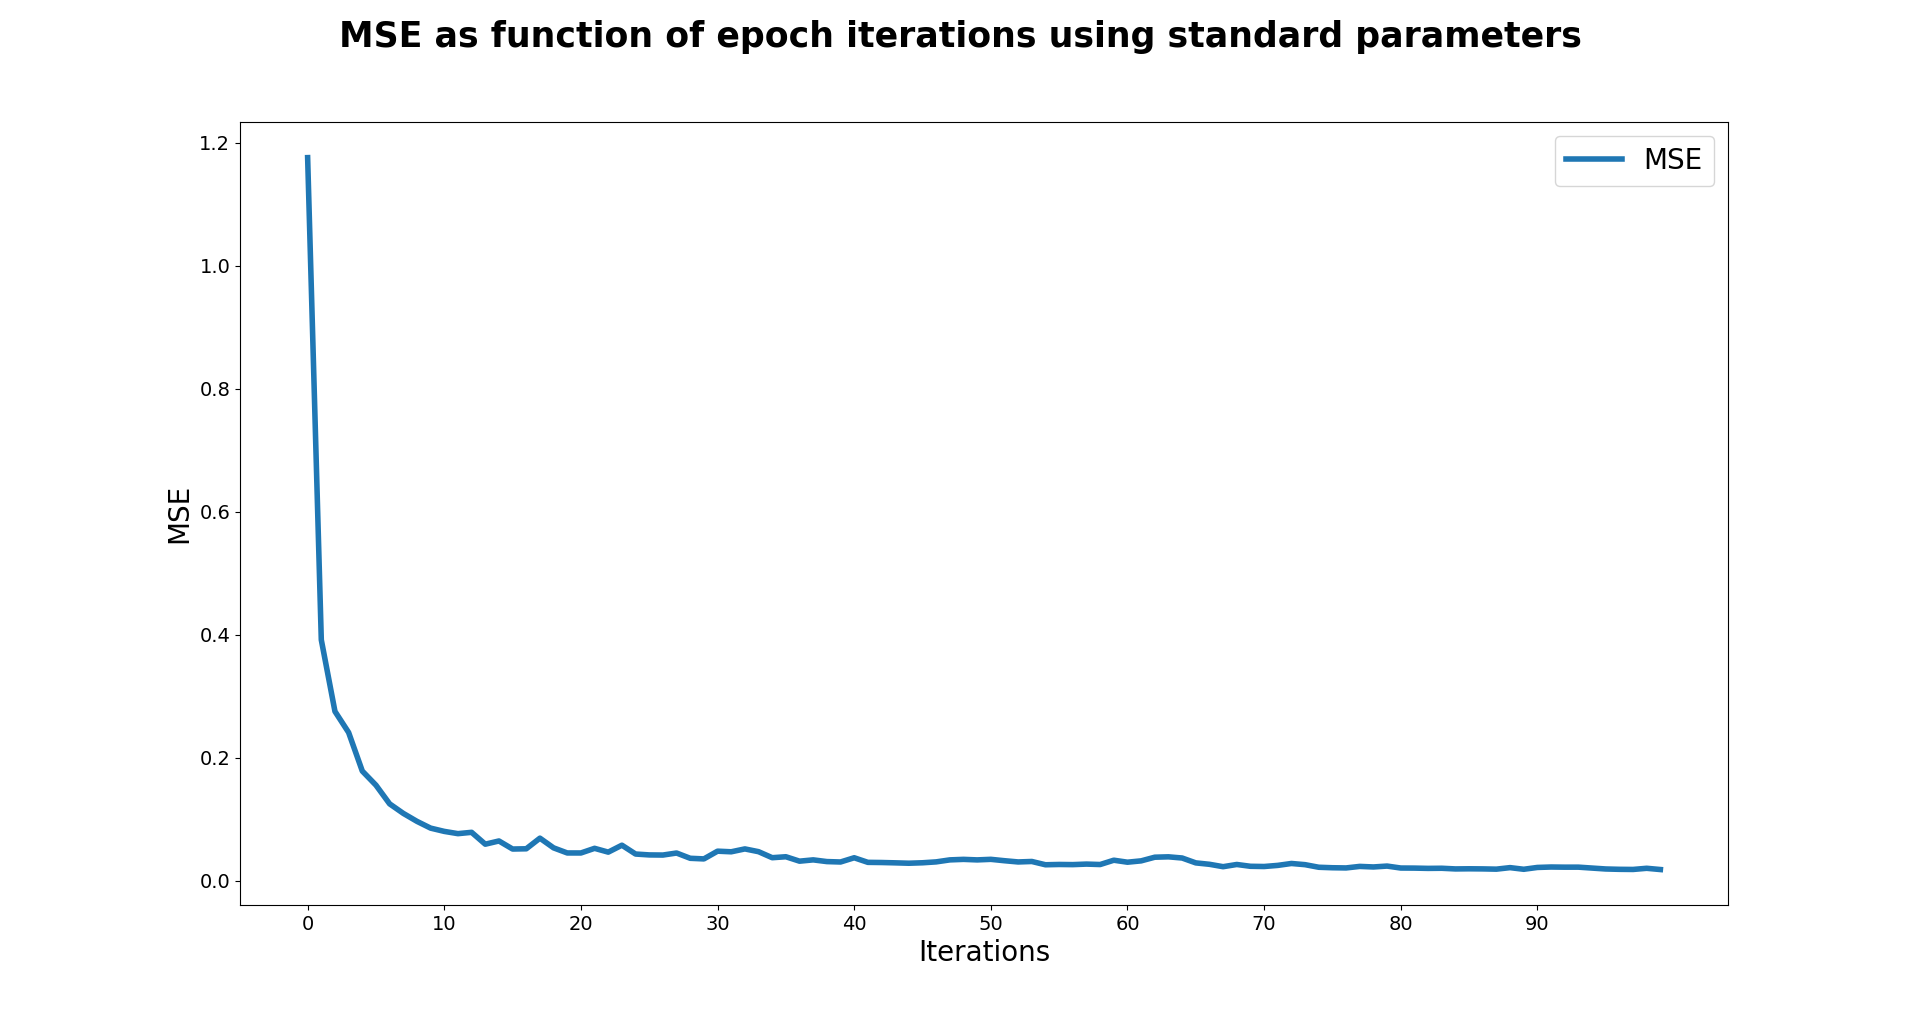
\includegraphics[width = 1\linewidth]{C:/Users/Sander/Documents/GitHub/FYS-STK4155/Project2/Project2/Report/Figures/MSEvsEPOCH_StandardRIDGE.PNG}
\caption{\label{fig:MSEvsEPOCHstandardRidge} The MSE as function of number of epoch iterations using static learning rate and Ridge equivalent SGD.}
\end{figure}

\noindent Figures \ref{fig:MSEvsEPOCHstandard} and \ref{fig:MSEvsEPOCHstandardRidge} shows that the MSE drastically increases as function of the number of epoch iterations, particularly at low number of iterations. At higher number of iterations, say around 30, the MSE keeps decreasing, but at a lower rate. One can also observe that the Ridge SGD starts at a lower MSE than the OLS SGD which indicate that Ridge algorithms fits the data better. Let us now see how the MSE changes as function of both epoch iterations and the size of the batch. We will then use the standard parameters, but change the batch size in the span $[100, 10, 1]$ and the results are shown in figures \ref{fig:MSEvsEPOCHbatchOLS} and \ref{fig:MSEvsEPOCHbatchRIDGE}

\begin{figure}[H]
\centering
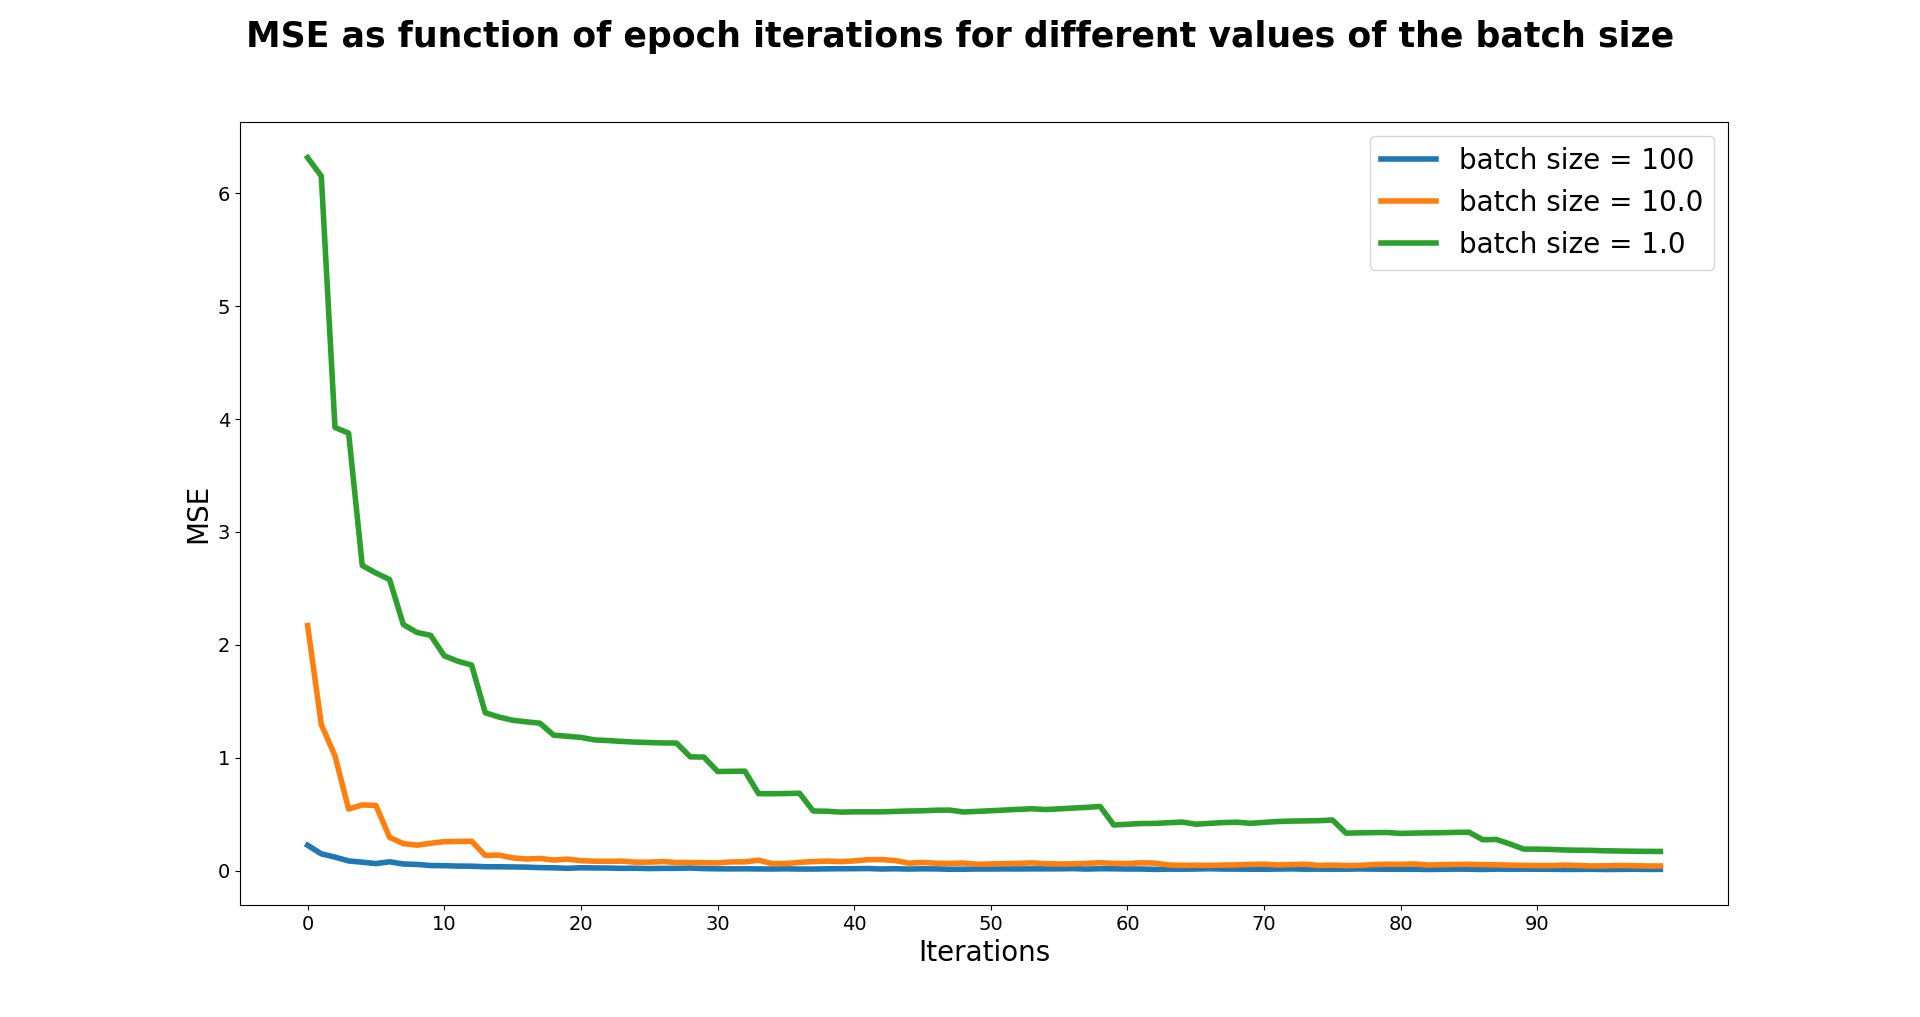
\includegraphics[width = 1\linewidth]{C:/Users/Sander/Documents/GitHub/FYS-STK4155/Project2/Project2/Report/Figures/MSEvsEPOCH_BatchOLS.PNG}
\caption{\label{fig:MSEvsEPOCHbatchOLS} The MSE as function of number of epoch iterations and batch sizes using static learning rate and OLS equivalent SGD.}
\end{figure}

\begin{figure}[H]
\centering
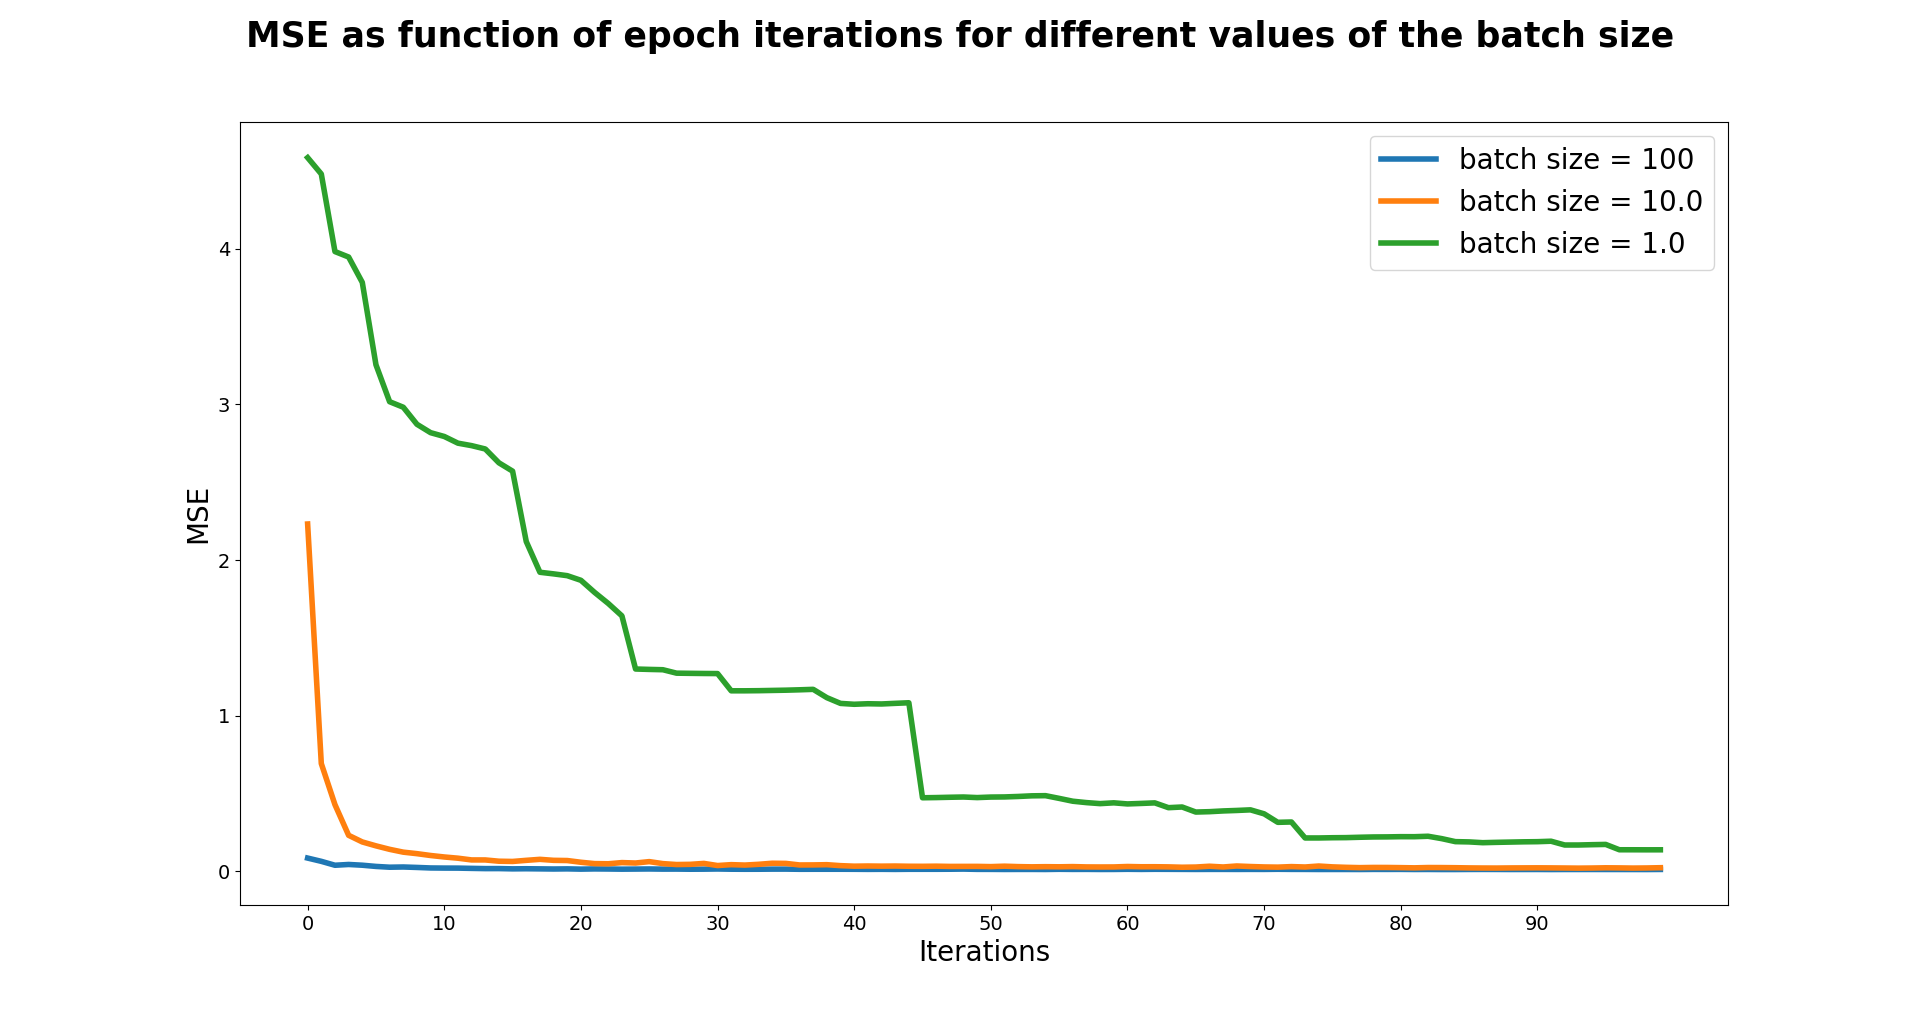
\includegraphics[width = 1\linewidth]{C:/Users/Sander/Documents/GitHub/FYS-STK4155/Project2/Project2/Report/Figures/MSEvsEPOCH_BatchRIDGE.PNG}
\caption{\label{fig:MSEvsEPOCHbatchRIDGE} The MSE as function of number of epoch iterations and batch sizes using static learning rate and Ridge equivalent SGD.}
\end{figure}

\noindent It can be observed from figures \ref{fig:MSEvsEPOCHbatchOLS} and \ref{fig:MSEvsEPOCHbatchRIDGE} that increasing the batch size drastically decreases the MSE. The batch size of 100 is equivalent to gradient descent (we use all observations) and it clearly has the lowest MSE for both the OLS and Ridge SGD. However, using the entirety of the data set can be extremely costly in terms of computational power, so it is not optimal for large data sets. What we also observe is that the difference in MSE between the batch sizes decreases for higher number of epoch iterations. In other words, we can utilize smaller batch sizes as long as we have a sufficiently large epoch. 
\\
Now let us see how the MSE varies as function of learning rate. We can again plot the MSE versus epoch iterations with our standard parameters, but vary the learning rate in the span $[0.0001, 0.001, 0.01]$

\begin{figure}[H]
\centering
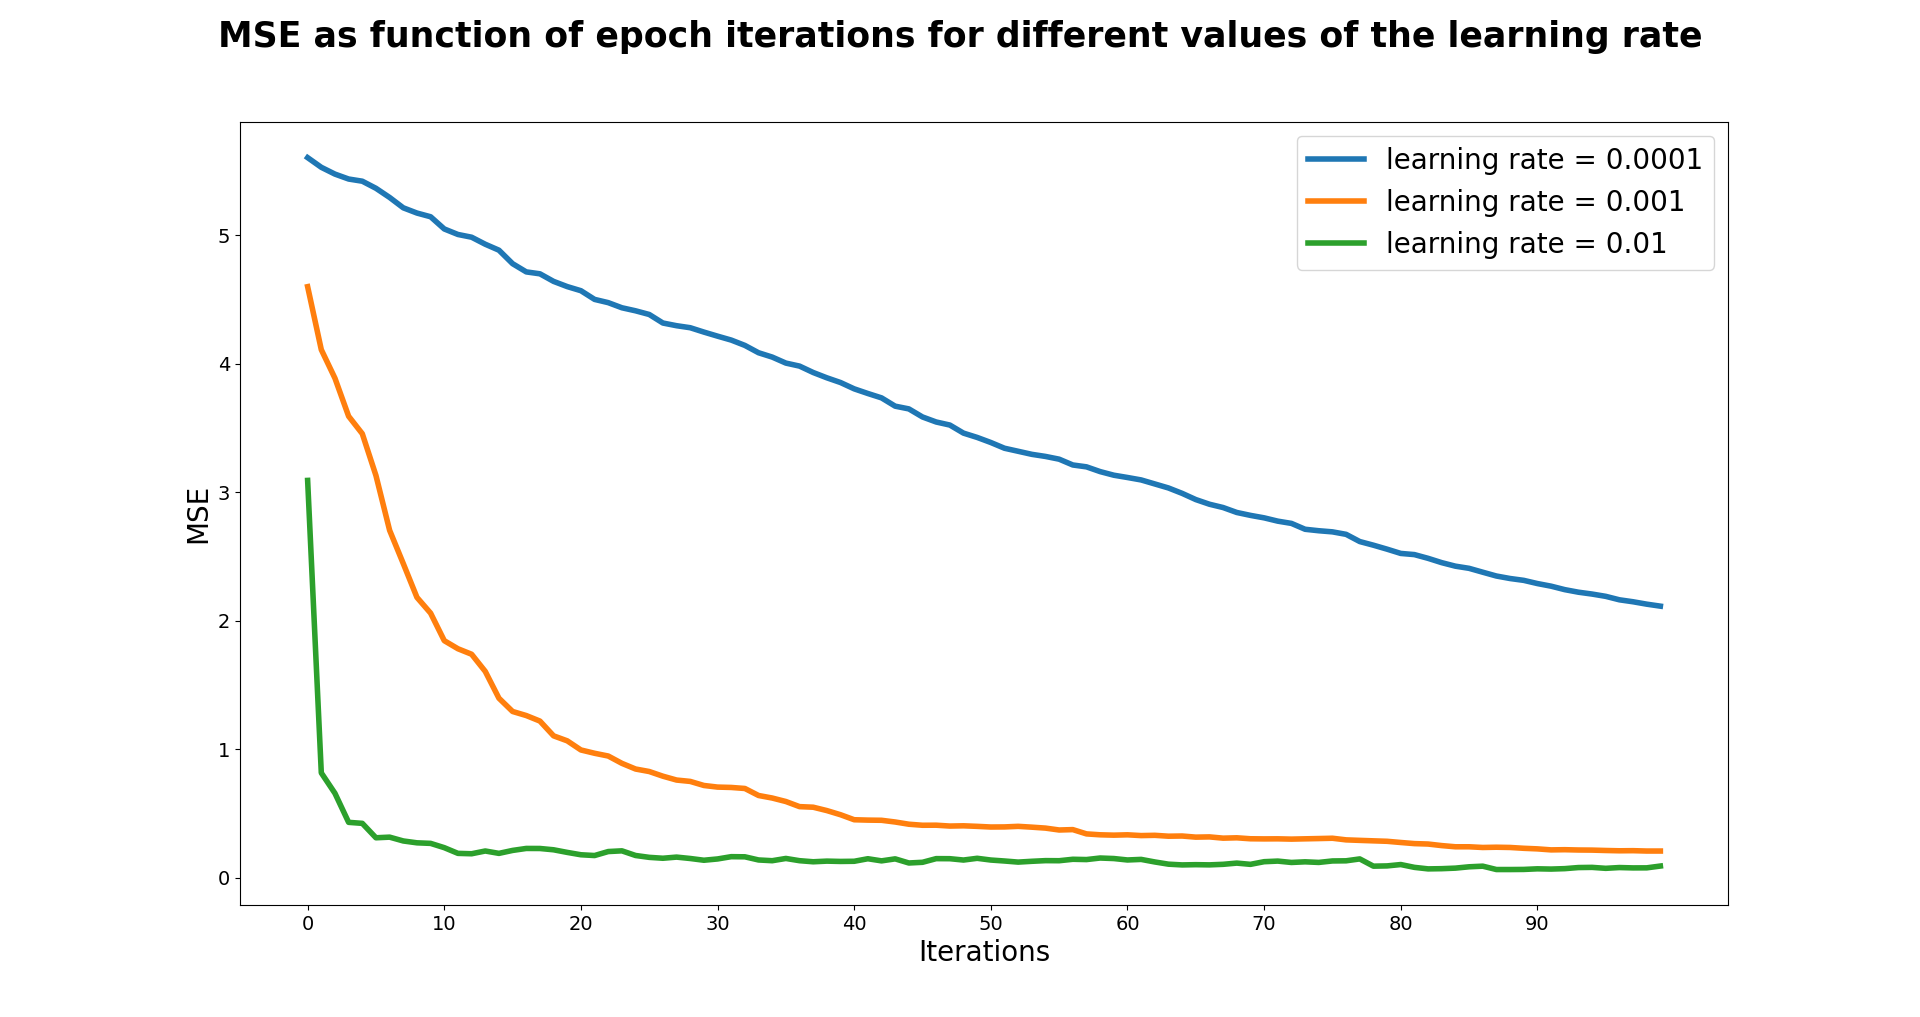
\includegraphics[width = 1\linewidth]{C:/Users/Sander/Documents/GitHub/FYS-STK4155/Project2/Project2/Report/Figures/MSEvsEPOCH_LearnOLS.PNG}
\caption{\label{fig:MSEvsEPOCHlaernOLS} The MSE as function of number of epoch iterations and learning rates using static learning rate and OLS equivalent SGD.}
\end{figure}

\begin{figure}[H]
\centering
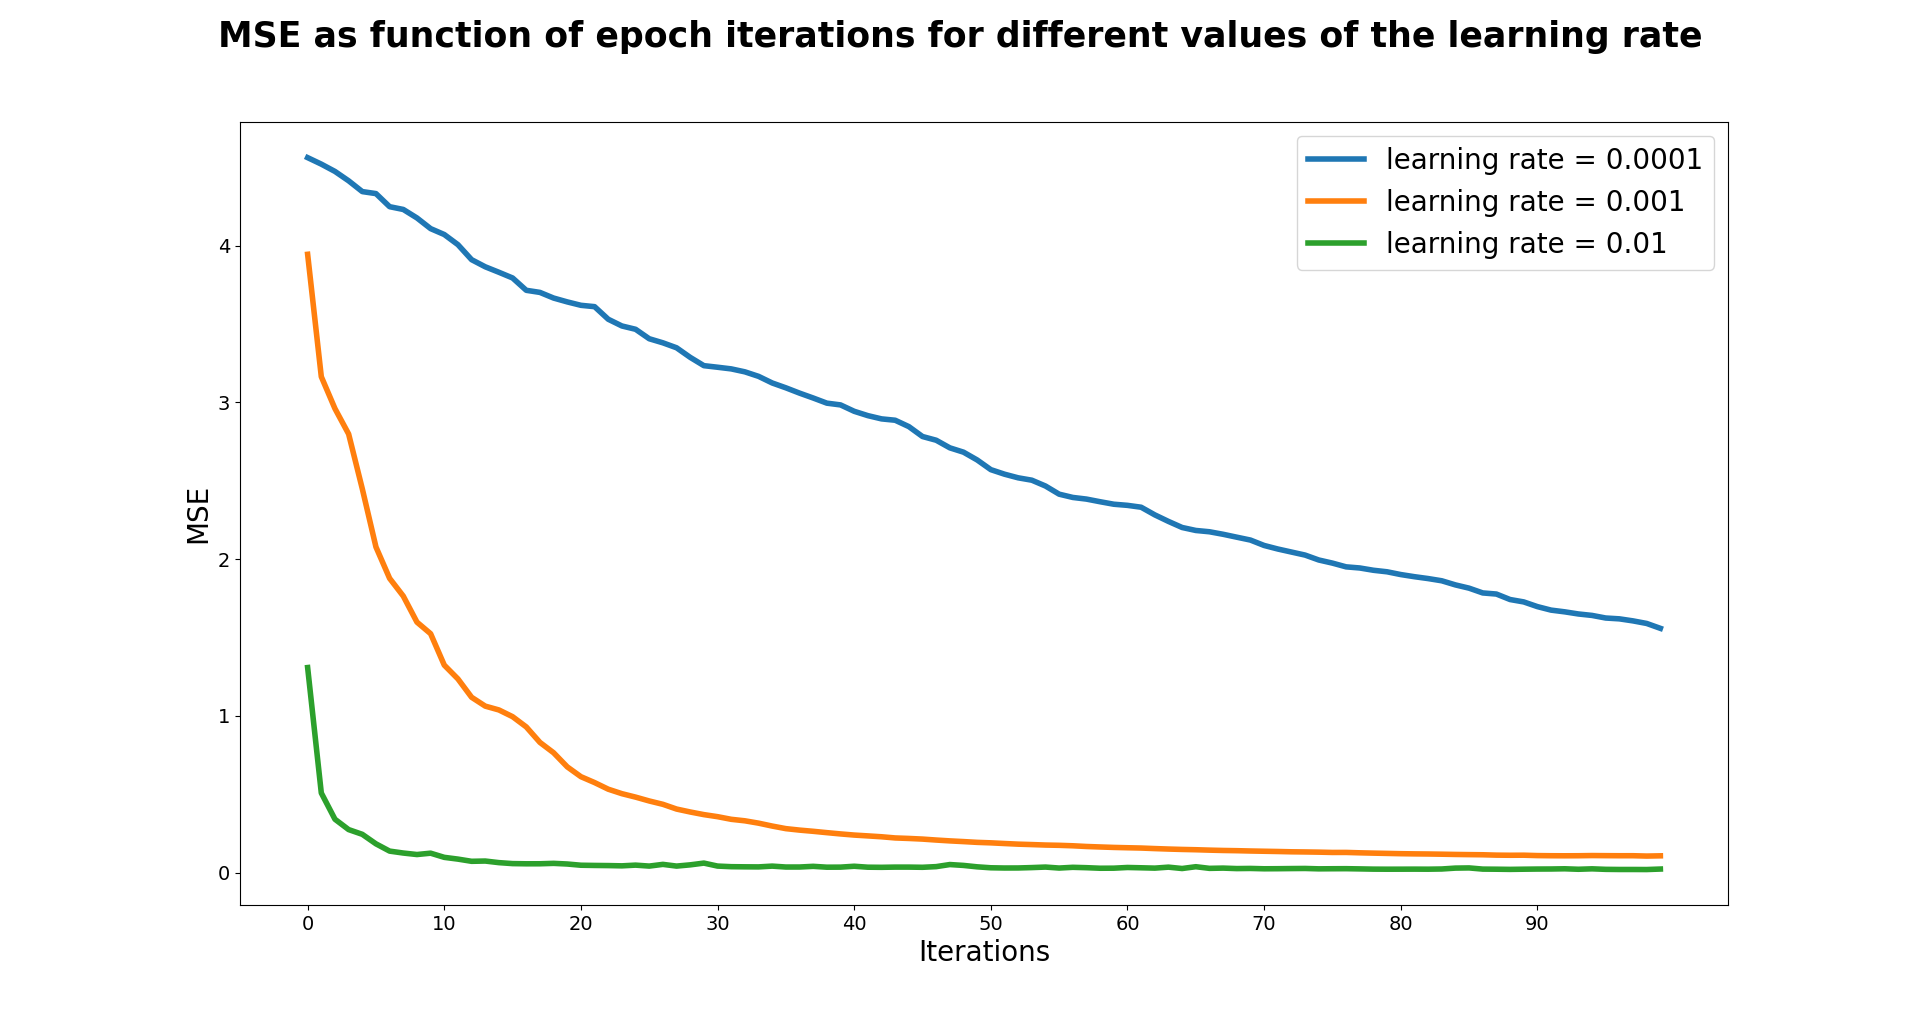
\includegraphics[width = 1\linewidth]{C:/Users/Sander/Documents/GitHub/FYS-STK4155/Project2/Project2/Report/Figures/MSEvsEPOCH_LearnRIDGE.PNG}
\caption{\label{fig:MSEvsEPOCHlearnRIDGE} The MSE as function of number of epoch iterations and learning rates using static learning rate and Ridge equivalent SGD.}
\end{figure}

\noindent One can observe from figures \ref{fig:MSEvsEPOCHlaernOLS} and \ref{fig:MSEvsEPOCHlearnRIDGE} that increasing the learning rate decreases the MSE for a low number of epoch iterations. However, the MSE of learning rates $0.01$ and $0.001$ converge for a higher number of epoch iterations. The MSE of the learning rate $0.0001$ does not drop exponentially, but linearly. This may be due to the learning rate is so small that the SGD takes a very long time to reach any kind of minimum, making the process too slow for the number of epoch iterations shown here. What we observe overall is that a learning rate anywhere over $0.001$ is fine as long as we have sufficiently many epoch iterations. 
\\
We can also study the how the MSE of the Ridge SGD changes as function of the number of epoch iterations and the penalty parameter $\lambda$. We again use the standard parameters but change the penalty parameter in the span $[0.0001, 0.001, 0.01, 0.1, 1]$ and the results are shown in figure \ref{fig:MSEvsEPOCHlambRIDGE}

\begin{figure}[H]
\centering
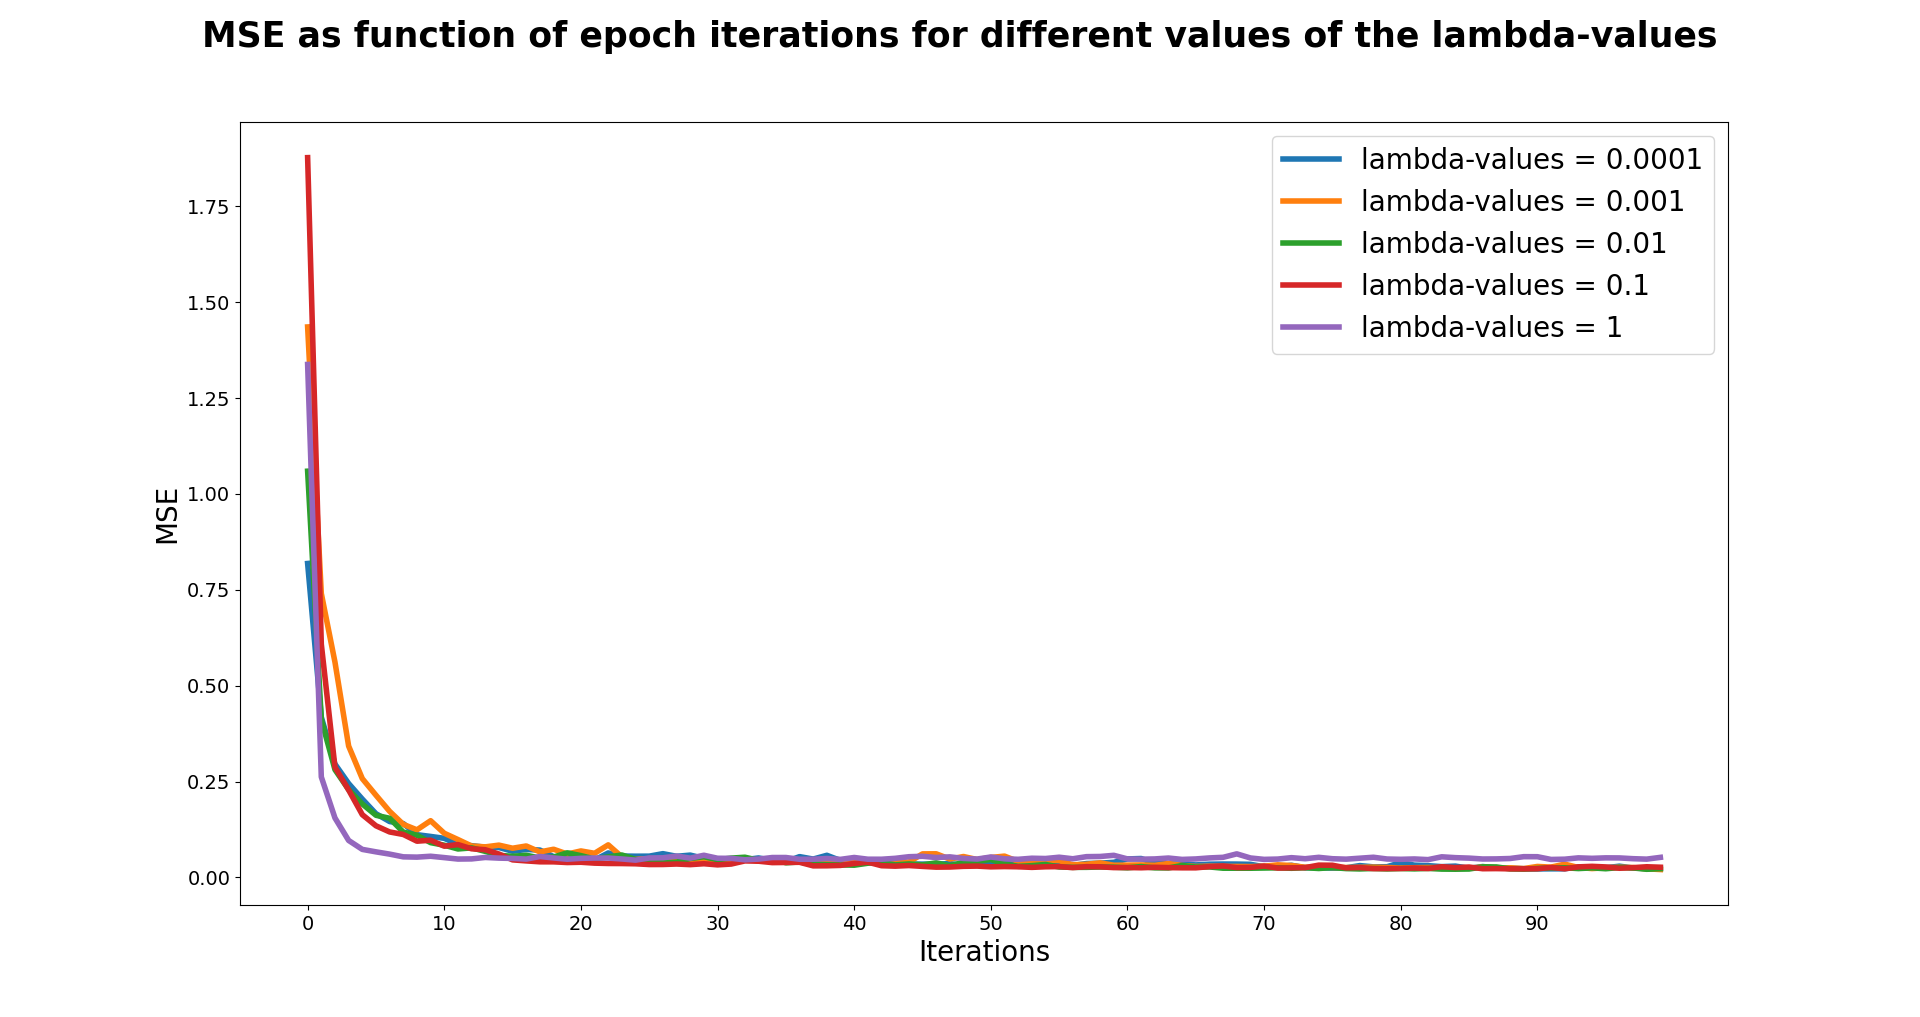
\includegraphics[width = 1\linewidth]{C:/Users/Sander/Documents/GitHub/FYS-STK4155/Project2/Project2/Report/Figures/MSEvsEPOCH_lambRIDGE.PNG}
\caption{\label{fig:MSEvsEPOCHlambRIDGE} The MSE as function of number of epoch iterations and penalty parameter $\lambda$ using static learning rate and Ridge equivalent SGD.}
\end{figure}

\noindent One can observe from figure \ref{fig:MSEvsEPOCHlambRIDGE} that the different penalty parameters yields similar results. One interesting observations is that the penalty parameter of $1$ yields the lowest MSE for a low number of epoch iterations, while it yields the highest MSE for a high number of epoch iterations. This may be caused by the fact that some of the regression coefficients are set close to zero and therefore do not contribute much to the overall cost function. It may be that the minimum of this reduced cost function has a minimum or local minimum with higher MSE than that of the less reduced cost function.

\begin{center}
\large{\textbf{Parameter dependencies for scheduled learning rate}}
\end{center}

\noindent We now aim to repeat the above analysis, but with a scheduled/adaptive learning rate. The learning rate will change as according to $\frac{t_0}{t+t_1}$ where $t_0 = 5$, $t_1 = 50$ and where t is constantly changing as function of epoch and batch iterations such that $t = $ current epoch iteration $\times$ batch size $+$ current batch iteration. The hopes for the scheduled learning rate is that we take large steps when we are far from the minimum of the cost function, while we take smaller steps as we approach said minimum. This will decrease our chances of getting "stuck" in some local minimum as our steps are too large for us to find ourselves in such a local minimum. We can implement this schedule in the SGD algorithm and see how the MSE changes for different epoch iterations and varying parameters. We start by simply plotting the MSE as function of epoch iteration using the standard parameters of table \ref{tab:standardParam}

\begin{figure}[H]
\centering
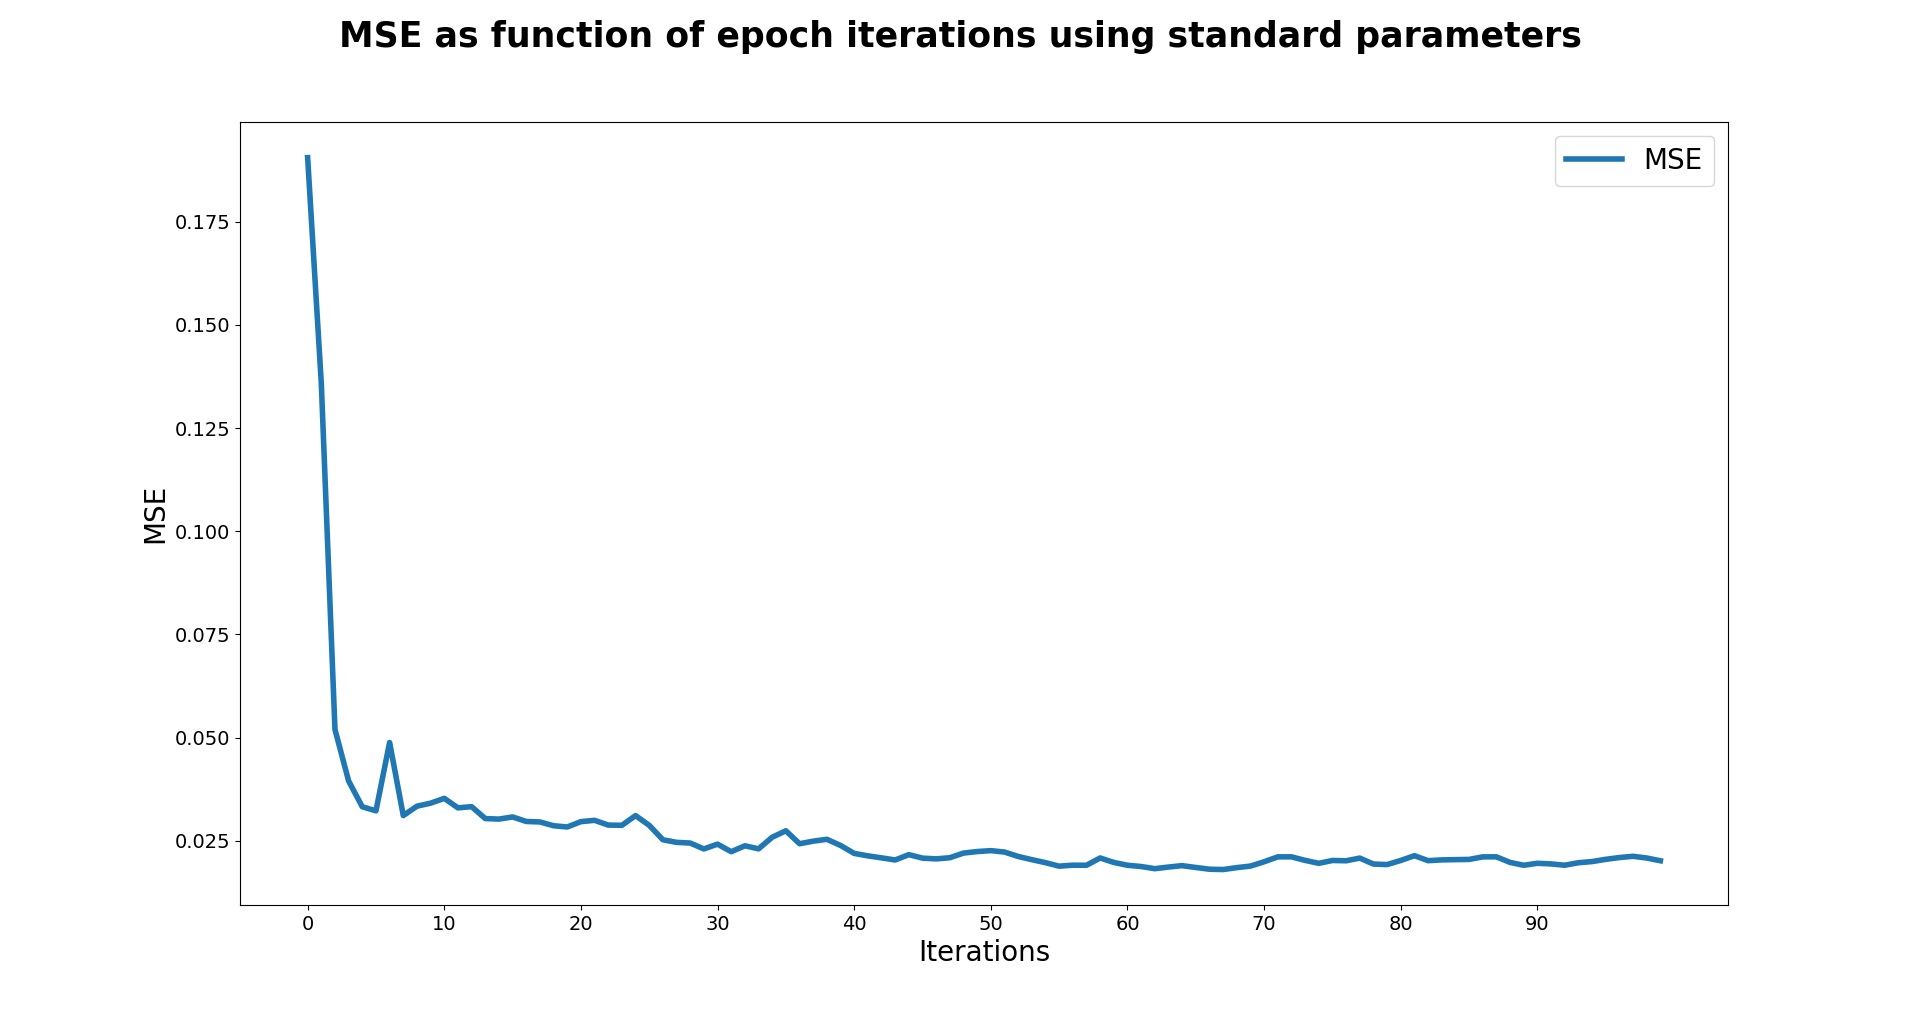
\includegraphics[width = 1\linewidth]{C:/Users/Sander/Documents/GitHub/FYS-STK4155/Project2/Project2/Report/Figures/MSEvsEPOCH_StandardOLS_schedule.PNG}
\caption{\label{fig:MSEvsEPOCHstandard_sch} The MSE as function of number of epoch iterations using a learning schedule rate and OLS equivalent SGD.}
\end{figure}

\begin{figure}[H]
\centering
\includegraphics[width = 1\linewidth]{C:/Users/Sander/Documents/GitHub/FYS-STK4155/Project2/Project2/Report/Figures/MSEvsEPOCH_StandardRIDGE_schedule.PNG}
\caption{\label{fig:MSEvsEPOCHstandardRidge_sch} The MSE as function of number of epoch iterations using a learning schedule rate and Ridge equivalent SGD.}
\end{figure}

\noindent It can be observed when comparing figures \ref{fig:MSEvsEPOCHstandard} and \ref{fig:MSEvsEPOCHstandardRidge} to figures \ref{fig:MSEvsEPOCHstandard_sch} and \ref{fig:MSEvsEPOCHstandardRidge_sch} that the MSE drops much quicker when we utilize a learning schedule. This is a direct consequence of taking larger steps when we are far away from the minimum. This ultimately leads to fewer steps to get to the minimum of the cost function. 
\\
We can also study how the MSE changes as function of batch size when we utilize a learning schedule and the result is plotted in figures QQQ and QQQ

\begin{figure}[H]
\centering
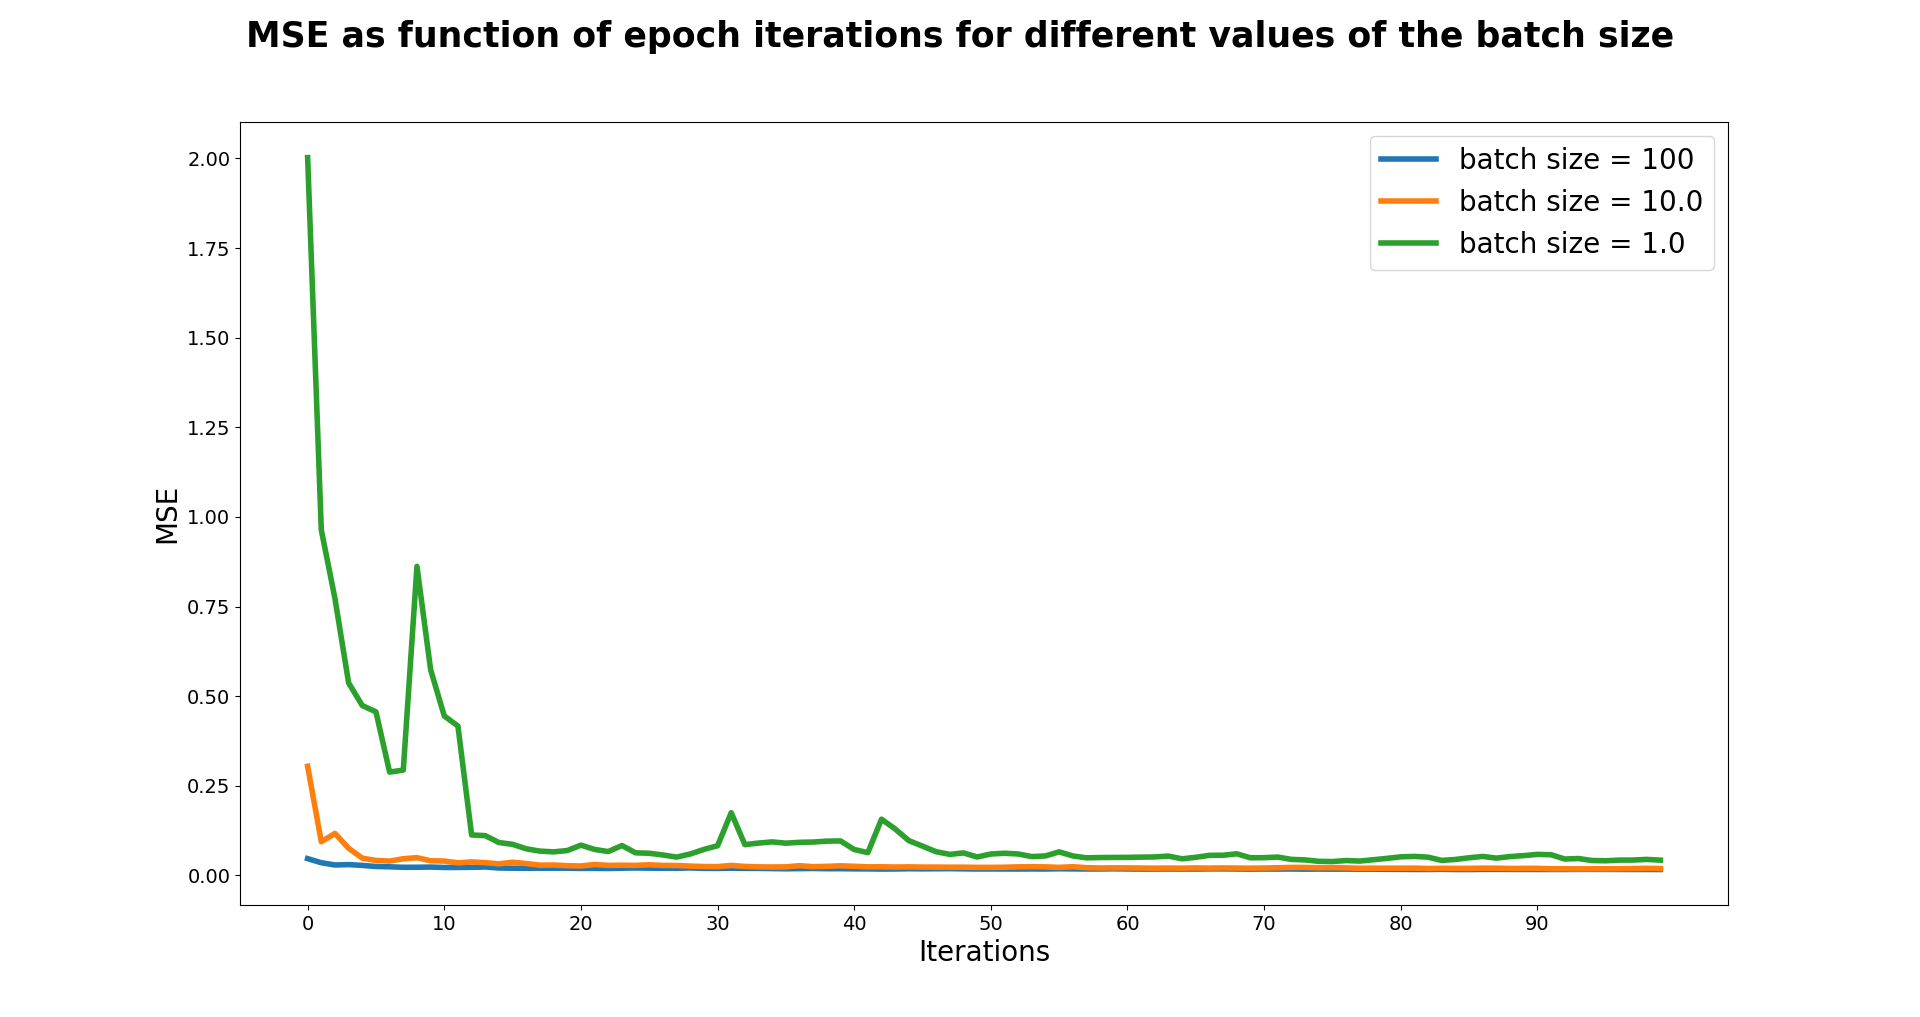
\includegraphics[width = 1\linewidth]{C:/Users/Sander/Documents/GitHub/FYS-STK4155/Project2/Project2/Report/Figures/MSEvsEPOCH_BatchOLS_schedule.PNG}
\caption{\label{fig:MSEvsEPOCHbatchOLS_sch} The MSE as function of number of epoch iterations and batch sizes using a learning schedule and OLS equivalent SGD.}
\end{figure}

\begin{figure}[H]
\centering
\includegraphics[width = 1\linewidth]{C:/Users/Sander/Documents/GitHub/FYS-STK4155/Project2/Project2/Report/Figures/MSEvsEPOCH_BatchRIDGE_schedule.PNG}
\caption{\label{fig:MSEvsEPOCHbatchRIDGE_sch} The MSE as function of number of epoch iterations and batch sizes using a learning schedule and Ridge equivalent SGD.}
\end{figure}

\noindent When we compare figures \ref{fig:MSEvsEPOCHbatchOLS} and \ref{fig:MSEvsEPOCHbatchRIDGE} to figures \ref{fig:MSEvsEPOCHbatchOLS_sch} and \ref{fig:MSEvsEPOCHbatchRIDGE_sch} we can observe that the batch size seems to play a more important role when using a learning schedule as the gap between batchs sizes are much greater than that of static learning rate. What is also observed is that the a batch size of one observation is much more "jagged" when we utilize a learning schedule. This be caused by the schedule "jumping" in and out of local minimums of the cost function. We can look at batch size equal to one for the OLS SGD in figure \ref{fig:MSEvsEPOCHbatchOLS_sch} where the MSE initially decreases a lot to around 5 iterations, but then has a large upturn in MSE. This may be one of these local minimum the algorithm found itself in. However, it does seem that the algorithm eventually finds the absolute minimum of the entire cost function as the "jagged" parts disappear for higher epoch iterations. 
\\
This phenomena seems to be a greater problem for the OLS as the Ridge SGD is nowhere near as jagged as the OLS SGD for batch size equal to one. This may be caused by the fact that some variables are reduced to a very small value, thereby removing any local minimum in that particular dimension.
\\
We can investigate the ridge implementation further by plotting plotting the MSE versus the epoch iterations for different values of the penalty parameter $\lambda$

\begin{figure}[H]
\centering
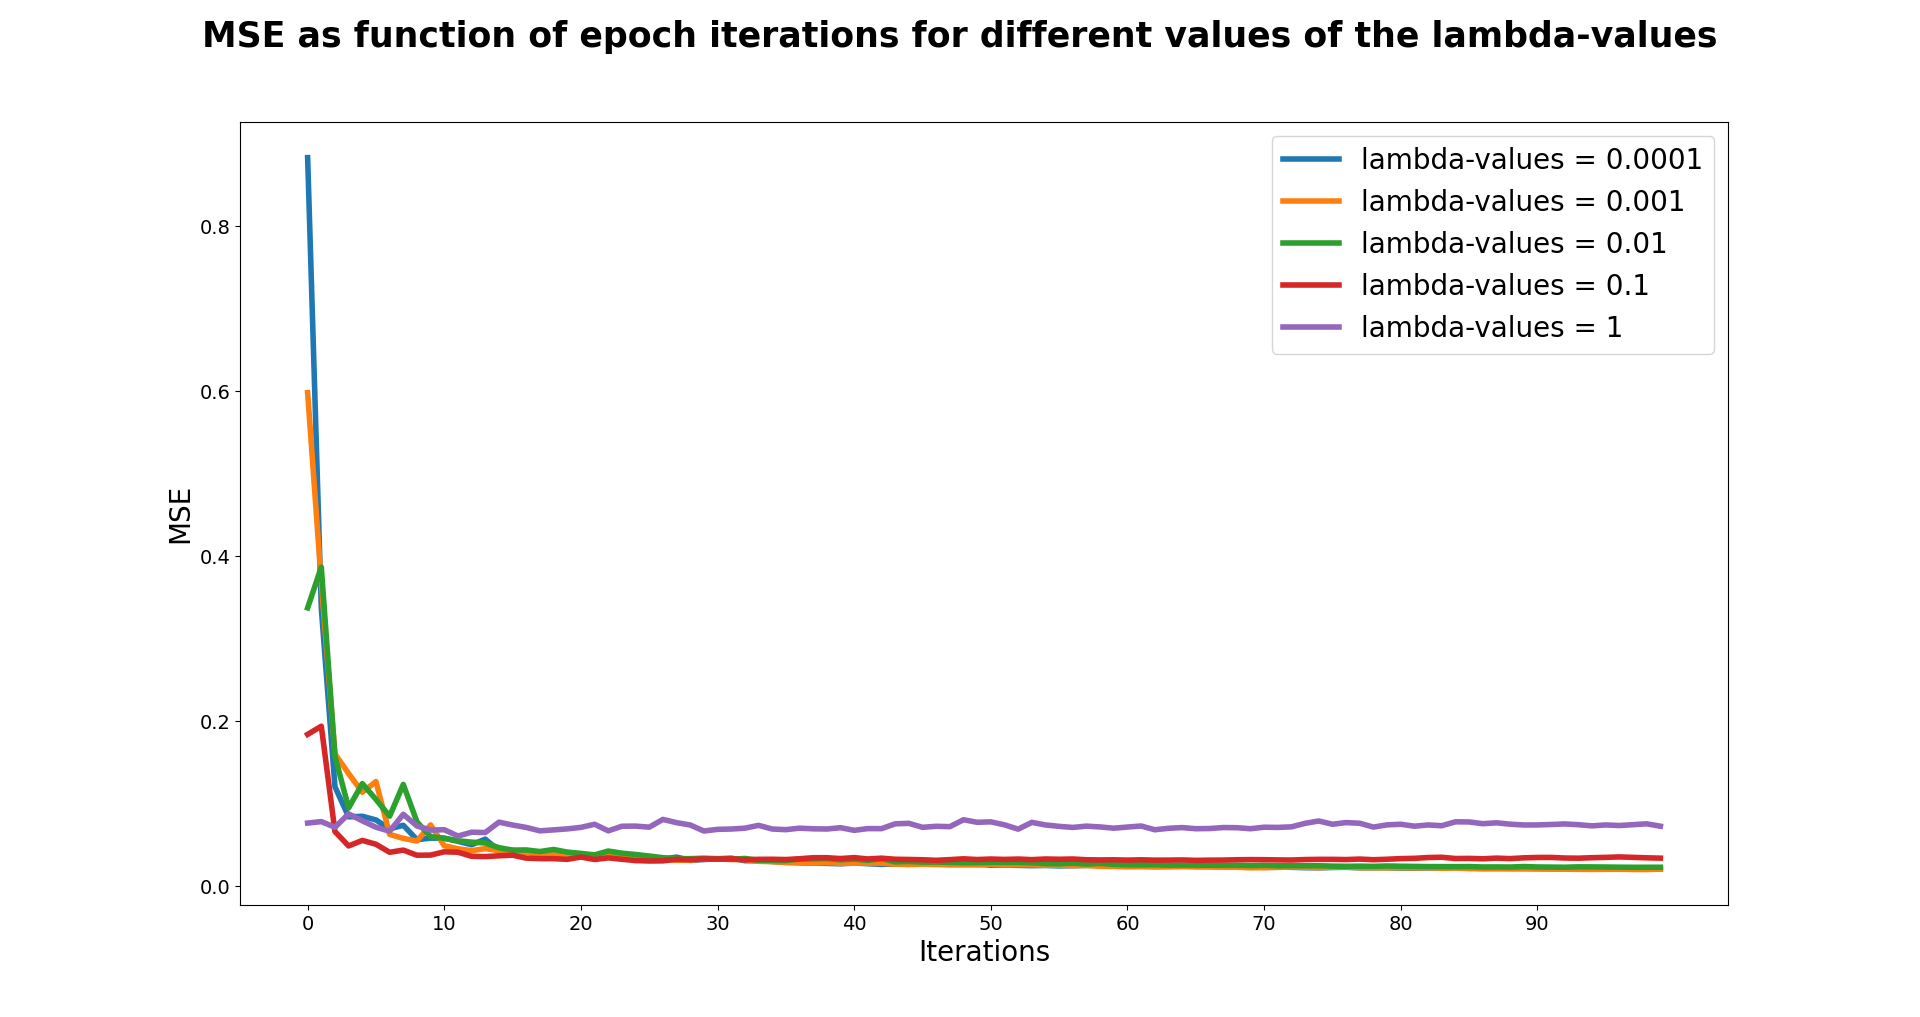
\includegraphics[width = 1\linewidth]{C:/Users/Sander/Documents/GitHub/FYS-STK4155/Project2/Project2/Report/Figures/MSEvsEPOCH_lambRIDGE_schedule.PNG}
\caption{\label{fig:MSEvsEPOCHlambRIDGE_sch} The MSE as function of number of epoch iterations and penalty parameter $\lambda$ using a learning schedule and Ridge equivalent SGD.}
\end{figure}

\begin{figure}[H]
\centering
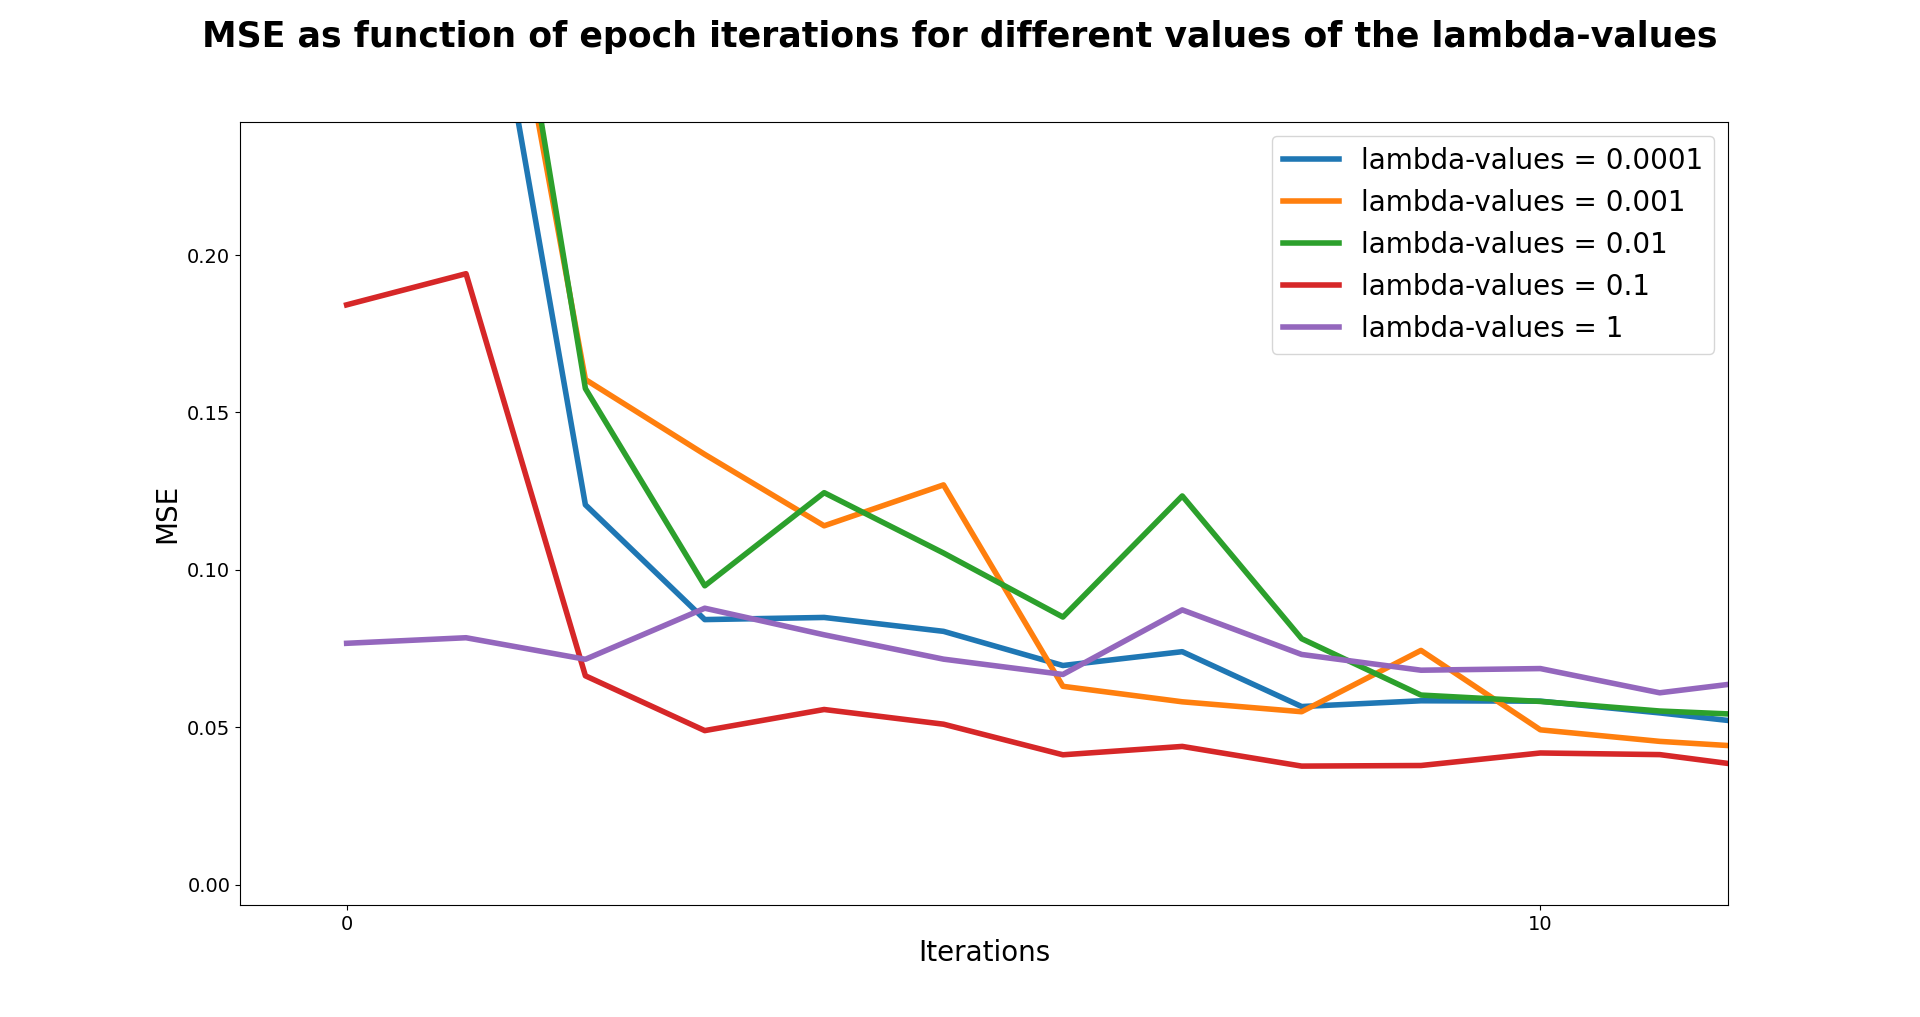
\includegraphics[width = 1\linewidth]{C:/Users/Sander/Documents/GitHub/FYS-STK4155/Project2/Project2/Report/Figures/MSEvsEPOCH_lambRIDGE_schedule2.PNG}
\caption{\label{fig:MSEvsEPOCHlambRIDGE_sch2} The MSE as function of number of epoch iterations and penalty parameter $\lambda$ using a learning schedule and Ridge equivalent SGD. This is a zoom-in of figure \ref{fig:MSEvsEPOCHlambRIDGE_sch}}.
\end{figure}

\noindent We can observe from figures that the choice of penalty parameter $\lambda$ has little or no effect on the MSE, except for when $\lambda = 1$. The MSE in this case never really increase or decrease, which is probably caused by the penalty term setting too many regression coefficients close to zero, meaning there is not really a minimum of the cost function since if all the regression coefficients are to small. 
\\
We also observe that the MSE for penalty parameters less than one decrease their MSE at a very low number of epoch iterations. Indicating that the minimum value is easy to find when some variables are very small.

\newpage

\begin{center}
\Large{\textbf{Exercise 1b)and 1c): Neural network for regression}}
\end{center}

\begin{center}
\large{\textbf{The basics of a neural network}}
\end{center}

\noindent A neural network is a concept based on how neurons operate in the brain where we have an input that travels through neurons that weights the input, eventually making its way to some given set of neuron that trigger an output. This process can be replicated by computers by creating a layered model consisting of one input layer where the data goes in, an output layer where the neural network prediction comes out and a given number of hidden layers consisting of hidden neurons. A conceptual drawing of this process can be seen in figure \ref{fig:nnconcept}

\begin{figure}[H]
\centering
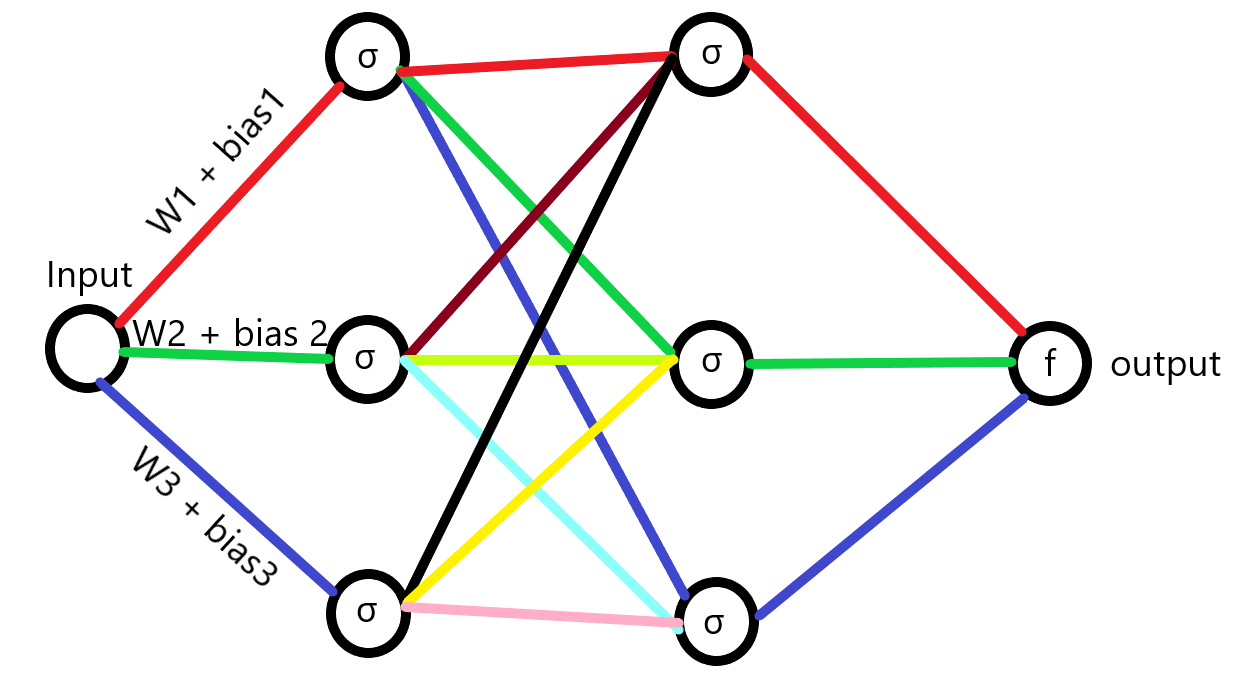
\includegraphics[width = 1\linewidth]{C:/Users/Sander/Documents/GitHub/FYS-STK4155/Project2/Project2/Report/Figures/NeuralNetConcept.PNG}
\caption{\label{fig:nnconcept} Conseptual drawing of a neural network. Here we have one input layer, two hidden layers and one output layer. The input and output layers consist of a single neuron, while the hidden layers have three neurons each. The input to each neuron is a weighted sum (W) plus a bias (B) from the previous layer. The output of a given neuron is the input to that neuron going through a activation function $\sigma$ which is then passed to the neurons in the next layer. The output activation function may be different than that of the neuron activation functions.}
\end{figure}

\noindent Figure \ref{fig:nnconcept} shows an input layer that passes a weighted sum plus bias to the three neurons in the first hidden layer. The weights $W_1, W_2$ and $W_3$ are typically different while the biases $B_1, B_2$ and $B_3$ are typically the equal. When these weighted sums plus bias enter a neuron, they are passed through an activation function which compresses the input to some value between zero and one. It is intuitive to think of this as how activated a neuron is, where one being fully activated and zero being fully inactivated. The data is passed through every neuron in every layer and will eventually reach the output layer where another activation function is applied. This whole process is called feed forward and is typically the first step of any neural network algorithm.
\\
The next step is to tune the weights within the neural network. This is where the gradient descent from exercise 1a) comes in. We can utilize the stochastic gradient descent to find the minimum of a cost function where each dimension is the weights of the neural network. Can then find which value of the weight would incrementally decrease the cost function, and then go back though our neural network and update the weight values in each neuron. This process is often called back propagation. We want to repeat the feed forward and back propagation many times in order for the weight to find their optimal value. This is called the training of the neural network. When we have trained the neural network sufficiently, it can be used to predict new data the network has never seen before. With these processes in mind, we can implement an algorithm that performs feed forward and back propagation.

\begin{center}
\large{\textbf{The sigmoid activation function}}
\end{center}

\noindent Three types of activation functions within the hidden layers will be implemented, the first one being the sigmoid activation function which is given by equation \ref{eq:sig}

\begin{equation}\label{eq:sig}
\begin{aligned}
\frac{1}{1 + e^{-x}}
\end{aligned}
\end{equation}

\noindent It can be seen from the definition of the sigmoid function that whatever the value of x, the output is always somewhere between zero and one. We can utilize this to force the neurons to output a value between zero and one.

\begin{center}
\large{\textbf{The RELU activation functions}}
\end{center}

\noindent So far we have only utilized the sigmoid function in our hidden neurons as defined in equation \ref{eq:sig}. Now we want to experiment with two additional activation functions, namely the RELU and the leaky RELU defined in equation \ref{eq:RELU} and \ref{eq:leakyRELU}

\begin{equation}\label{eq:RELU}
\begin{aligned}
f(x) = 
\begin{cases}
x,& \text{if } x > 0\\
0,& \text{otherwise}
\end{cases}
\end{aligned}
\end{equation}

\begin{equation}\label{eq:leakyRELU}
\begin{aligned}
f(x) = 
\begin{cases}
x,& \text{if } x > 0\\
ax,& \text{otherwise}
\end{cases}
\end{aligned}
\end{equation}

\noindent We can see that this is close to the linear activation function where the input is simply passed through without any alterations. However, if the input is zero, then the output from a given neuron will be zero in the RELU case. The same goes for the leaky RELU case, but instead if setting the input values to zero, we set it to some small constant times the input. a in equation \ref{eq:leakyRELU} is typically in the range of $0.01$ and kind of has the same purpose as the bias in the way that it prevents the neuron from ever giving an output of zero (thereby the name "leaky"). Similar to the bias, this is done to prevent a chain of zeros to be passed through the neural network.
\\
One can observe from equations \ref{eq:RELU} and \ref{eq:leakyRELU} that the output from a given neuron will not be between zero and one if the input to the neuron is greater than zero. This has proven to be a problem when implementing the code as some configurations of the neural network will explode the gradient. The exploding gradient happens when 
\\
We can now perform the same analysis as in exercise 1b), but using the RELU and leaky RELU instead of the sigmoid as our hidden layer activation function.

\begin{center}
\large{\textbf{Learning rate, weights and biases}}
\end{center}

\noindent The neural network have proved stable when using the sigmoid activation function for the hidden layers as observed from the previous exercise. The leaky RELU and sometimes the RELU were prone to overflow leading to a worse predictions. The overflow became a huge problem for learning rates larger than 0.01, and therefore, only learning rates under this value were considered. Another solution to counter the overflow problem were increasing the number of epoch iterations to 2000 and decreasing the batch size to around 5. 
\\
It was also observed that the initial weights really impacted whether the network overflowed or not. Setting the initial weight to some random number drawn from a standard normal distribution gave severe flaws for many layer/neuron configurations. However, the xavier weight initialization proved to stabilize the network in most cases. The xavier weight initialization aims to maintain a constant variance of the data passing through the network (kilde). Doing this drastically reduced the chance for overflow which really showed when coding the network.
\\
The bias has in this case was simply been set to $0.01$. The role of the bias is to make sure there is some input to the neurons. Say a neuron only receives zeros from the previous layer. This would in turn lead to a feed forward of only zeros for that particular set of neurons meaning they will never contribute to the network. Therefore, it is important to add some bias to each neuron. The choice of bias showed to be of little significance when we played around with the code. The only important thing was that the bias was greater than zero, as a bias of zero often resulted in the network only passing zeros through, ultimately leading to a terrible prediction.

\begin{center}
\large{\textbf{Neural network results}}
\end{center}

\noindent We first want to see how the different activation function behave relative to the number of epoch iterations, the size of the batch and the learning rate. Figure \ref{fig:MSEvsLrateTOTAL1} and \ref{fig:MSEvsLrateTOTAL2} show the MSE and $R^2$ as function of learning rate using 100 epoch iterations and a batch size of 10 for the sigmoid, RELU and leaky RELU activation functions

\begin{figure}[H]
\centering
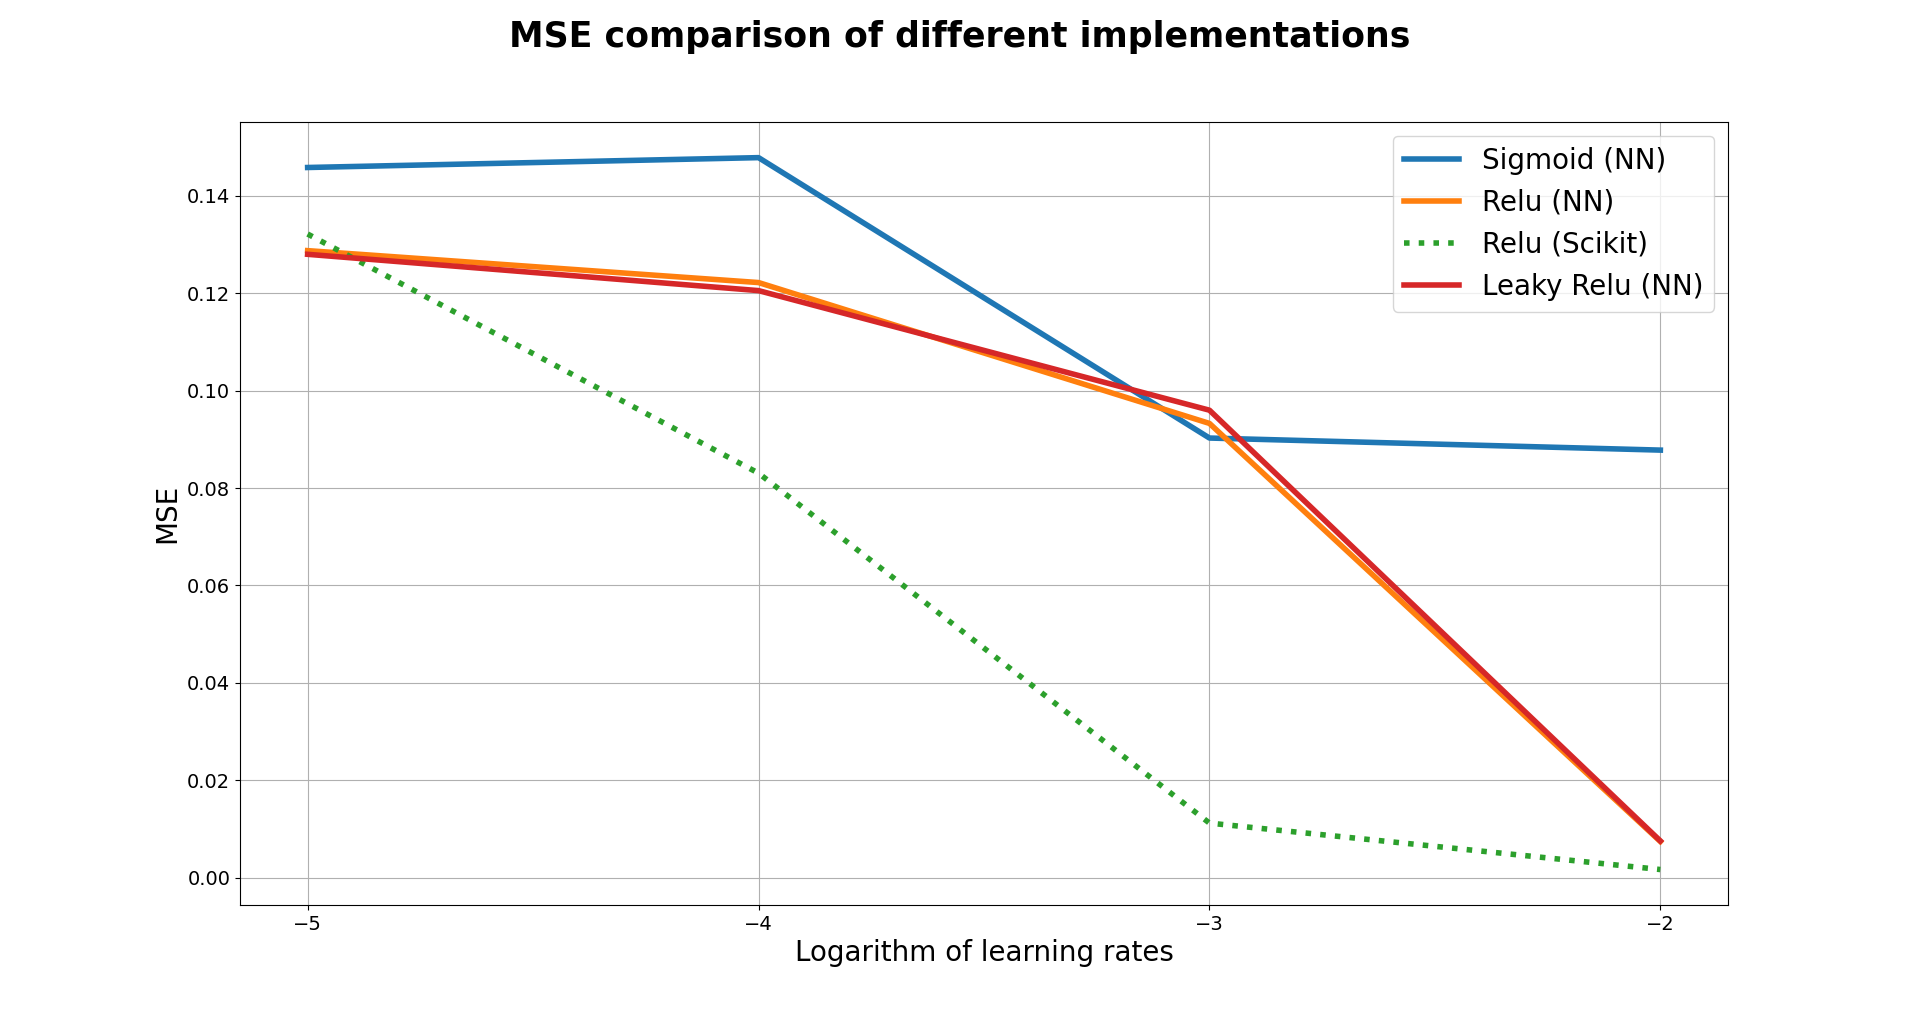
\includegraphics[width = 1\linewidth]{C:/Users/Sander/Documents/GitHub/FYS-STK4155/Project2/Project2/Report/Figures/MSEvsLearn_OLS_TOTAL_epoch100_batch10.PNG}
\caption{\label{fig:MSEvsLrateTOTAL1} The MSE as function of number of learning rate for the three activation functions when we utilize 100 epoch iterations and a batch size of 10. This is the OLS equivalent.}
\end{figure}

\begin{figure}[H]
\centering
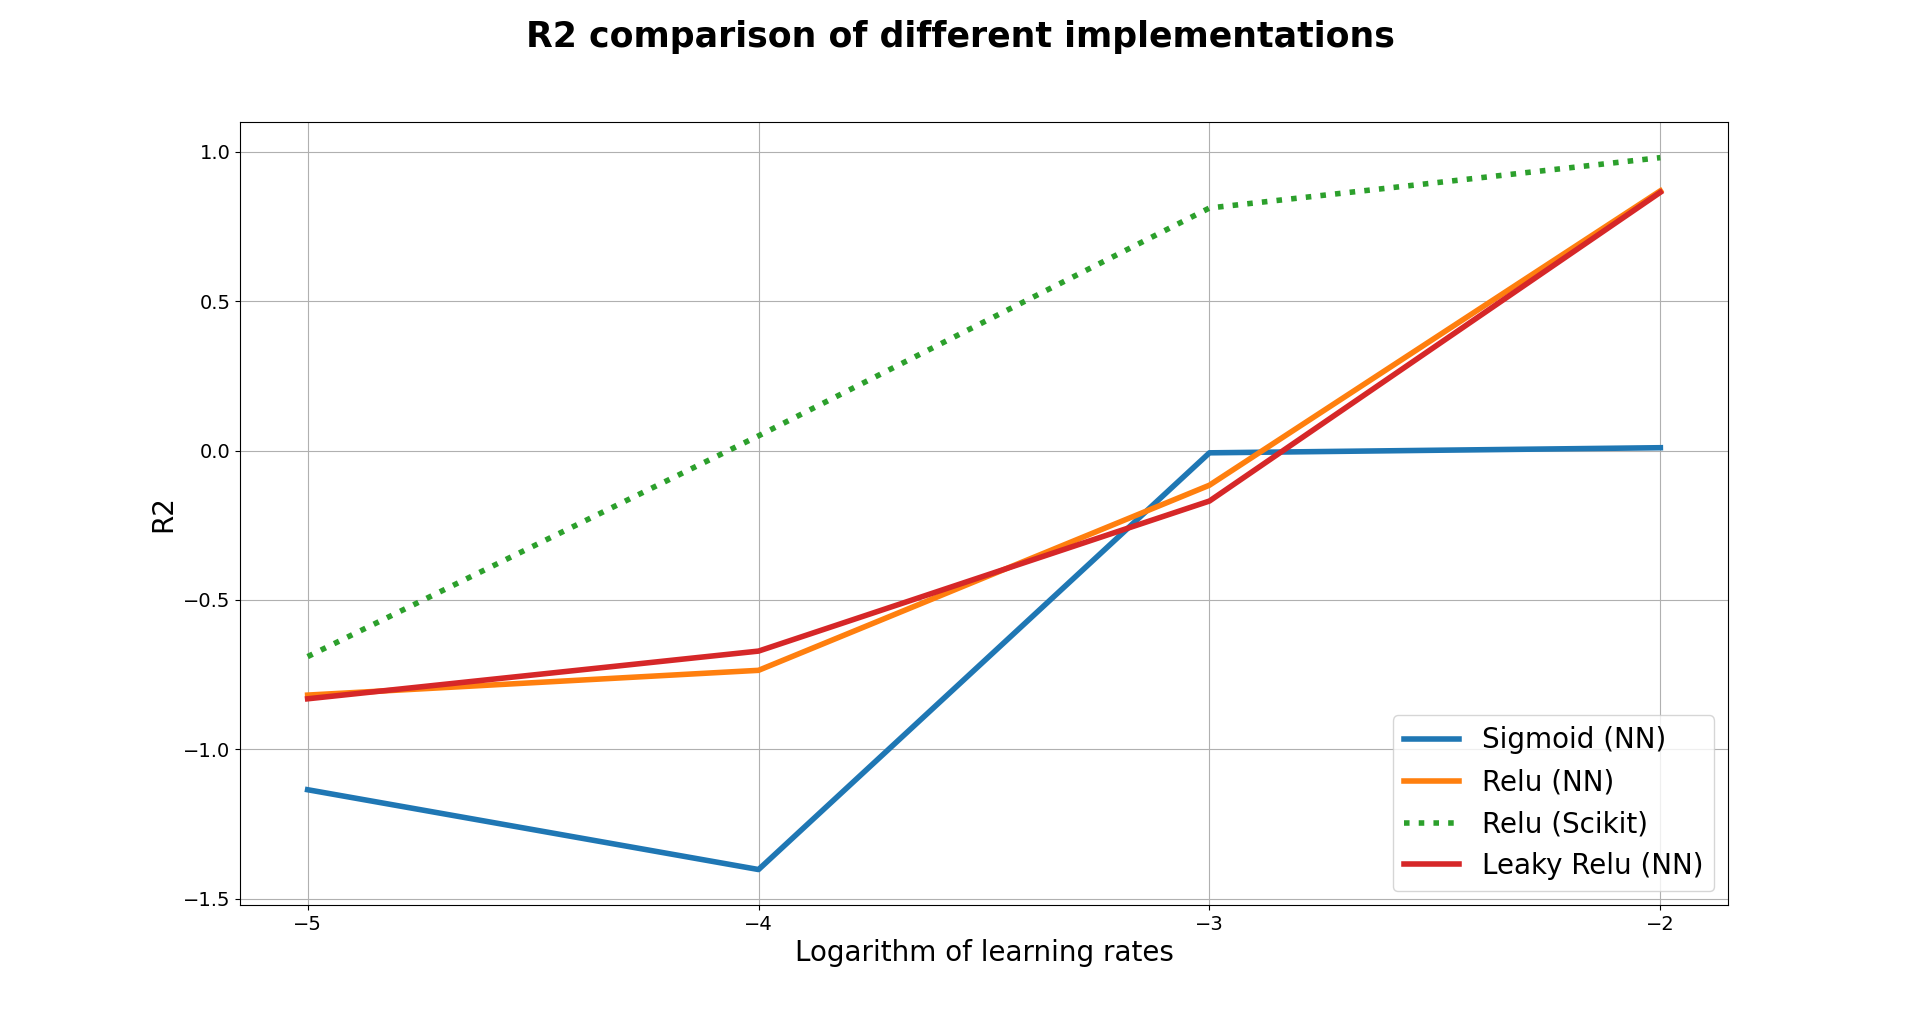
\includegraphics[width = 1\linewidth]{C:/Users/Sander/Documents/GitHub/FYS-STK4155/Project2/Project2/Report/Figures/MSEvsLearn_OLS_TOTAL_epoch100_batch10_r2.PNG}
\caption{\label{fig:MSEvsLrateTOTAL2} The $R^2$ as function of number of learning rate for the three activation functions when we utilize 100 epoch iterations and a batch size of 10. This is the OLS equivalent.}
\end{figure}

\noindent Figures \ref{fig:MSEvsLrateTOTAL1} and \ref{fig:MSEvsLrateTOTAL2} also include the Scikit implementation of the RELU activation function. It can be observed that the Scikit implementation outperforms my own neural network, particularly for lower learning rates. My own RELU and leaky RELU implementations seem nearly equivalent and are able to predict the test set much better than the sigmoid. It seems that the sigmoid implementation reaches a cap at $R^2 = 0$, which is equivalent to the baseline model. This means that the sigmoid model is just as good as randomly guessing the prediction. It can also be observed that the RELU implementations gets closer to the Scikit implementation for higher learning rates. We now aim to increase the number of epoch iterations from 100 to 500 as seen in figures \ref{fig:MSEvsLrateTOTAL3} and \ref{fig:MSEvsLrateTOTAL4}

\begin{figure}[H]
\centering
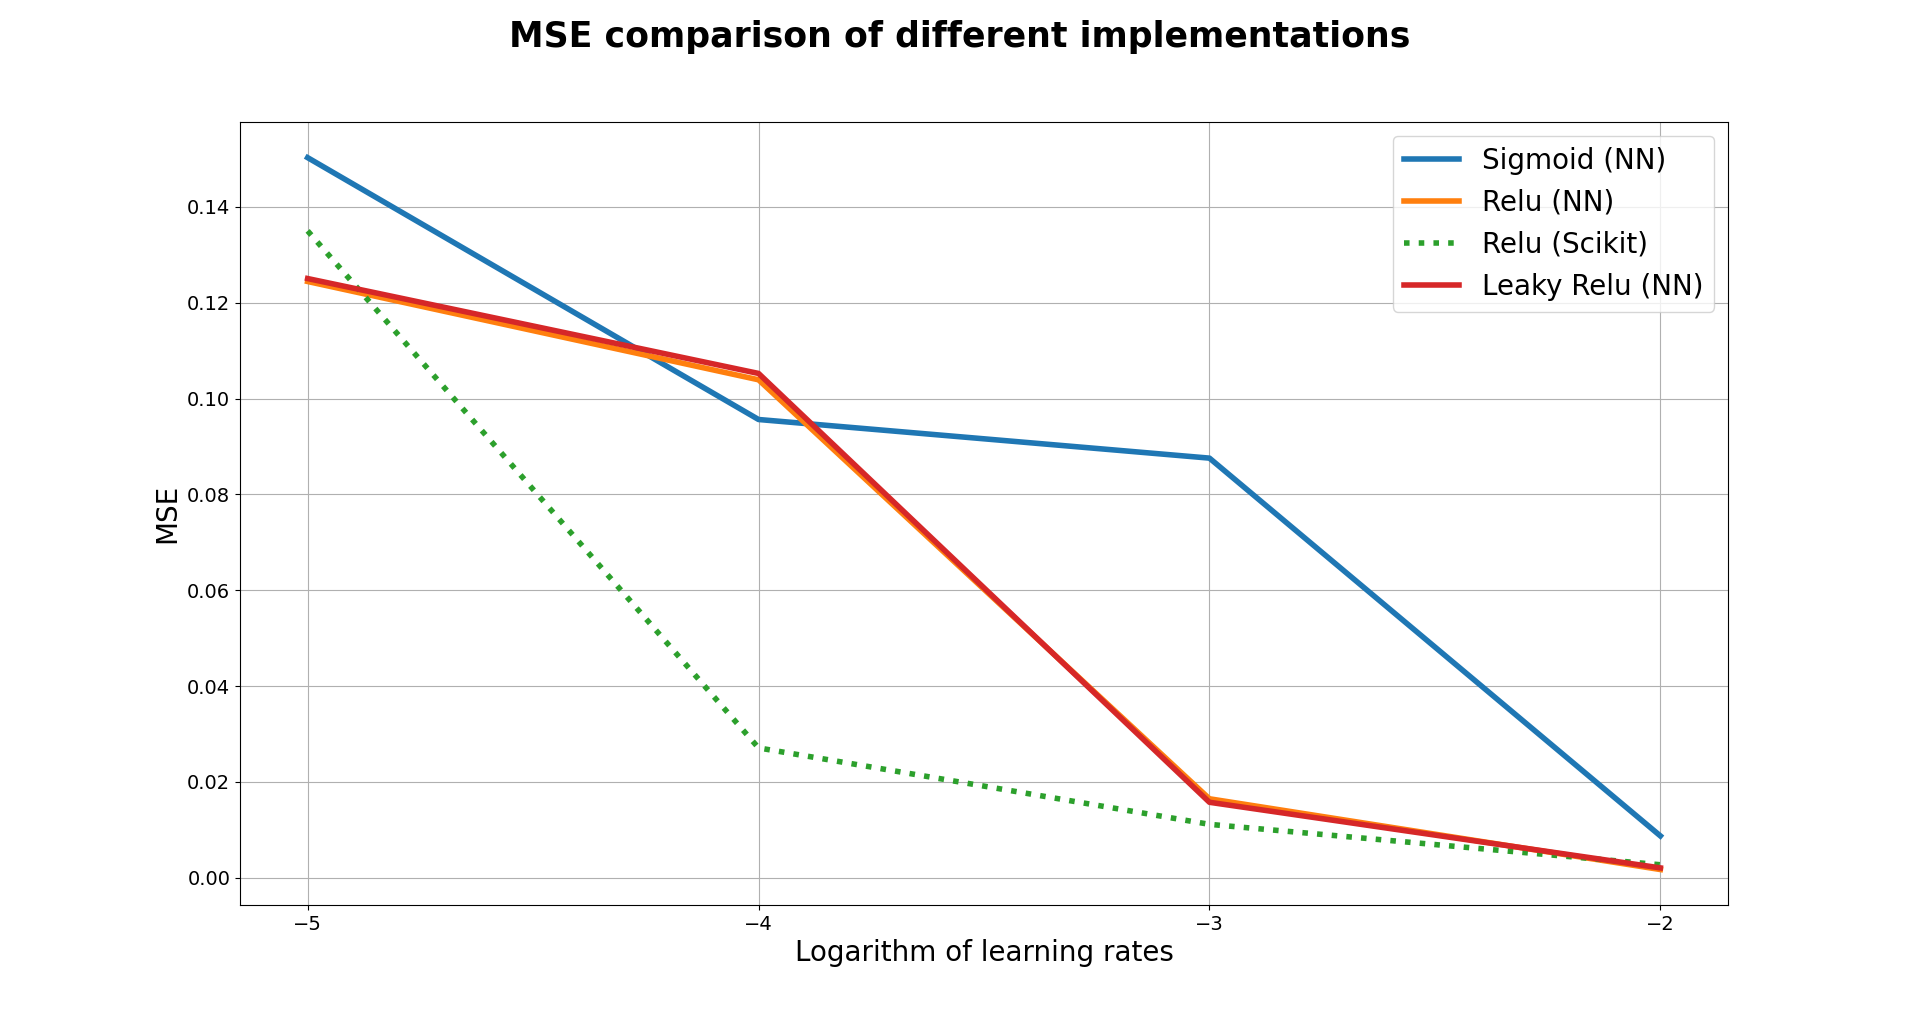
\includegraphics[width = 1\linewidth]{C:/Users/Sander/Documents/GitHub/FYS-STK4155/Project2/Project2/Report/Figures/MSEvsLearn_OLS_TOTAL_epoch500_batch10.PNG}
\caption{\label{fig:MSEvsLrateTOTAL3} The MSE as function of number of learning rate for the three activation functions when we utilize 500 epoch iterations and a batch size of 10. This is the OLS equivalent.}
\end{figure}

\begin{figure}[H]
\centering
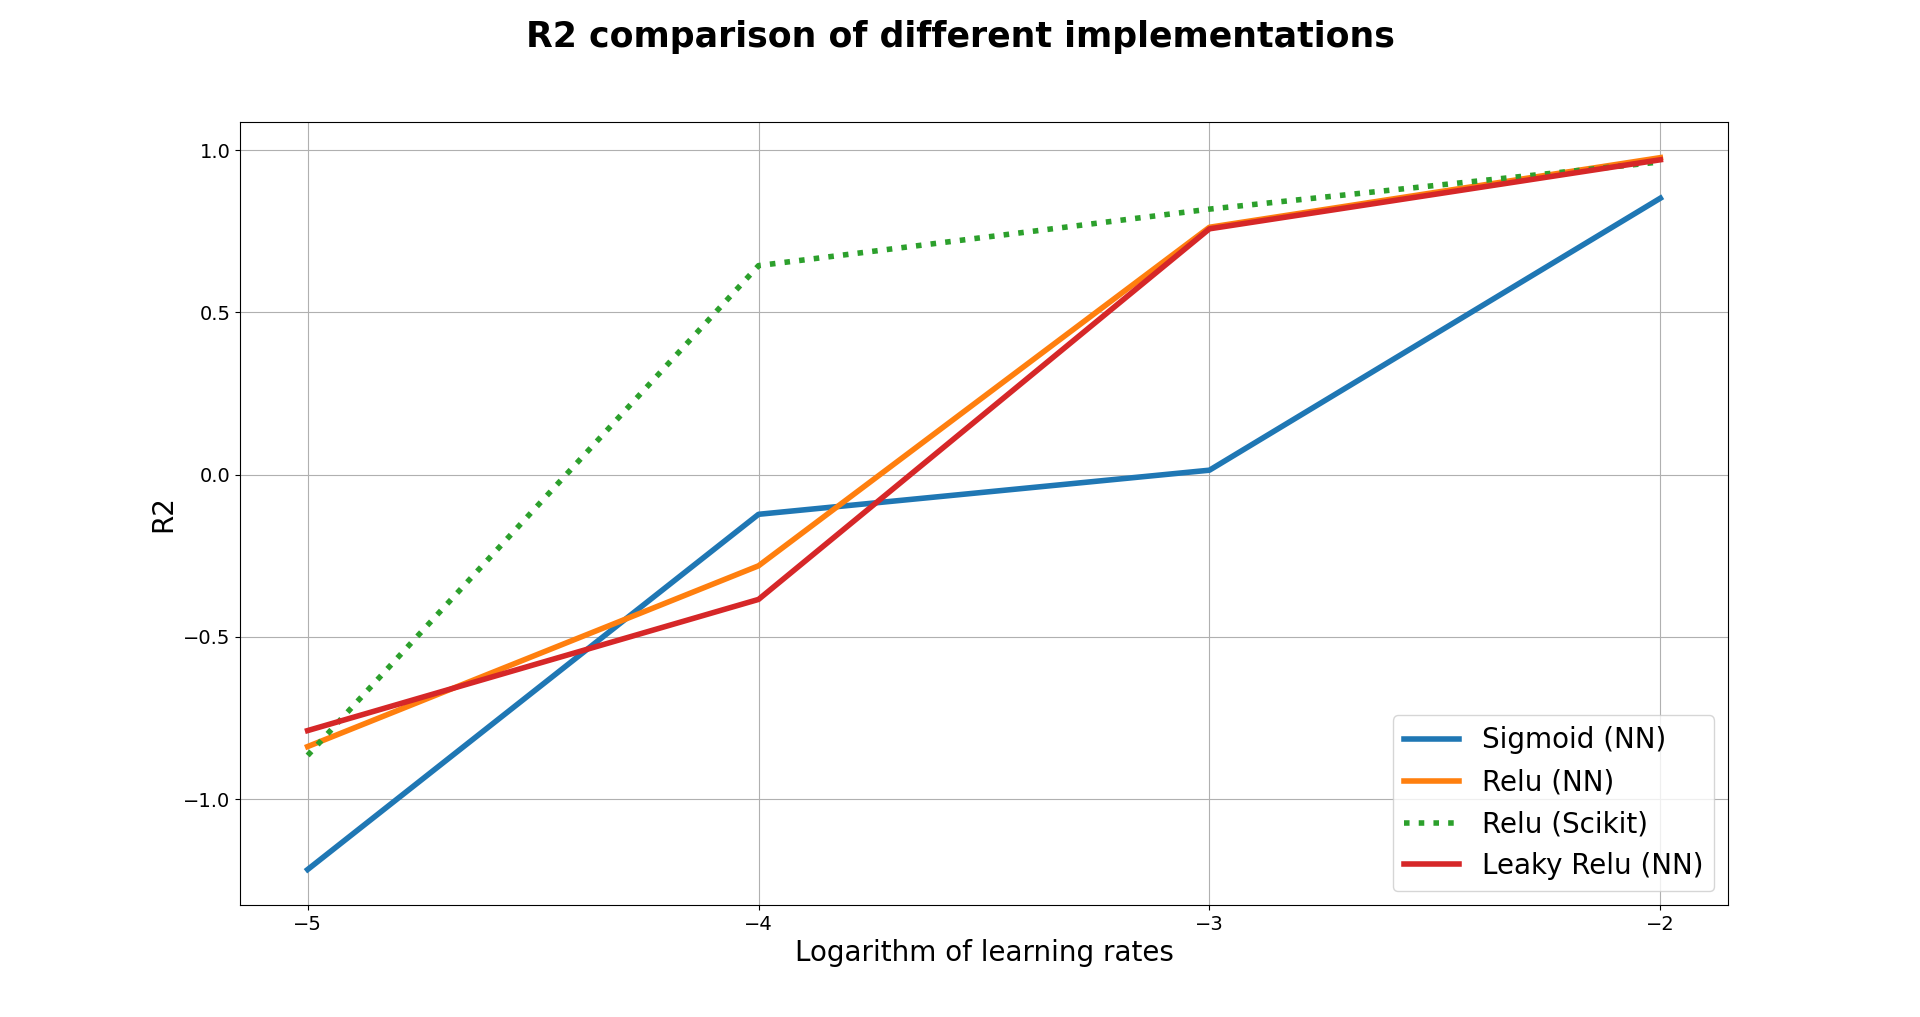
\includegraphics[width = 1\linewidth]{C:/Users/Sander/Documents/GitHub/FYS-STK4155/Project2/Project2/Report/Figures/MSEvsLearn_OLS_TOTAL_epoch500_batch10_r2.PNG}
\caption{\label{fig:MSEvsLrateTOTAL4} The $R^2$ as function of number of learning rate for the three activation functions when we utilize 500 epoch iterations and a batch size of 10. This is the OLS equivalent.}
\end{figure}

\noindent One can observe that increasing the number of epoch iterations caused the sigmoid implementation to perform better. It seems as going over some epoch threshold results in the sigmoid implementation breaking through the previously stated cap and it can therefore predict the test data better than the baseline. We now increase the number of epoch iterations from 500 to 2000 as seen in figures \ref{fig:MSEvsLrateTOTAL5} and \ref{fig:MSEvsLrateTOTAL6}

\begin{figure}[H]
\centering
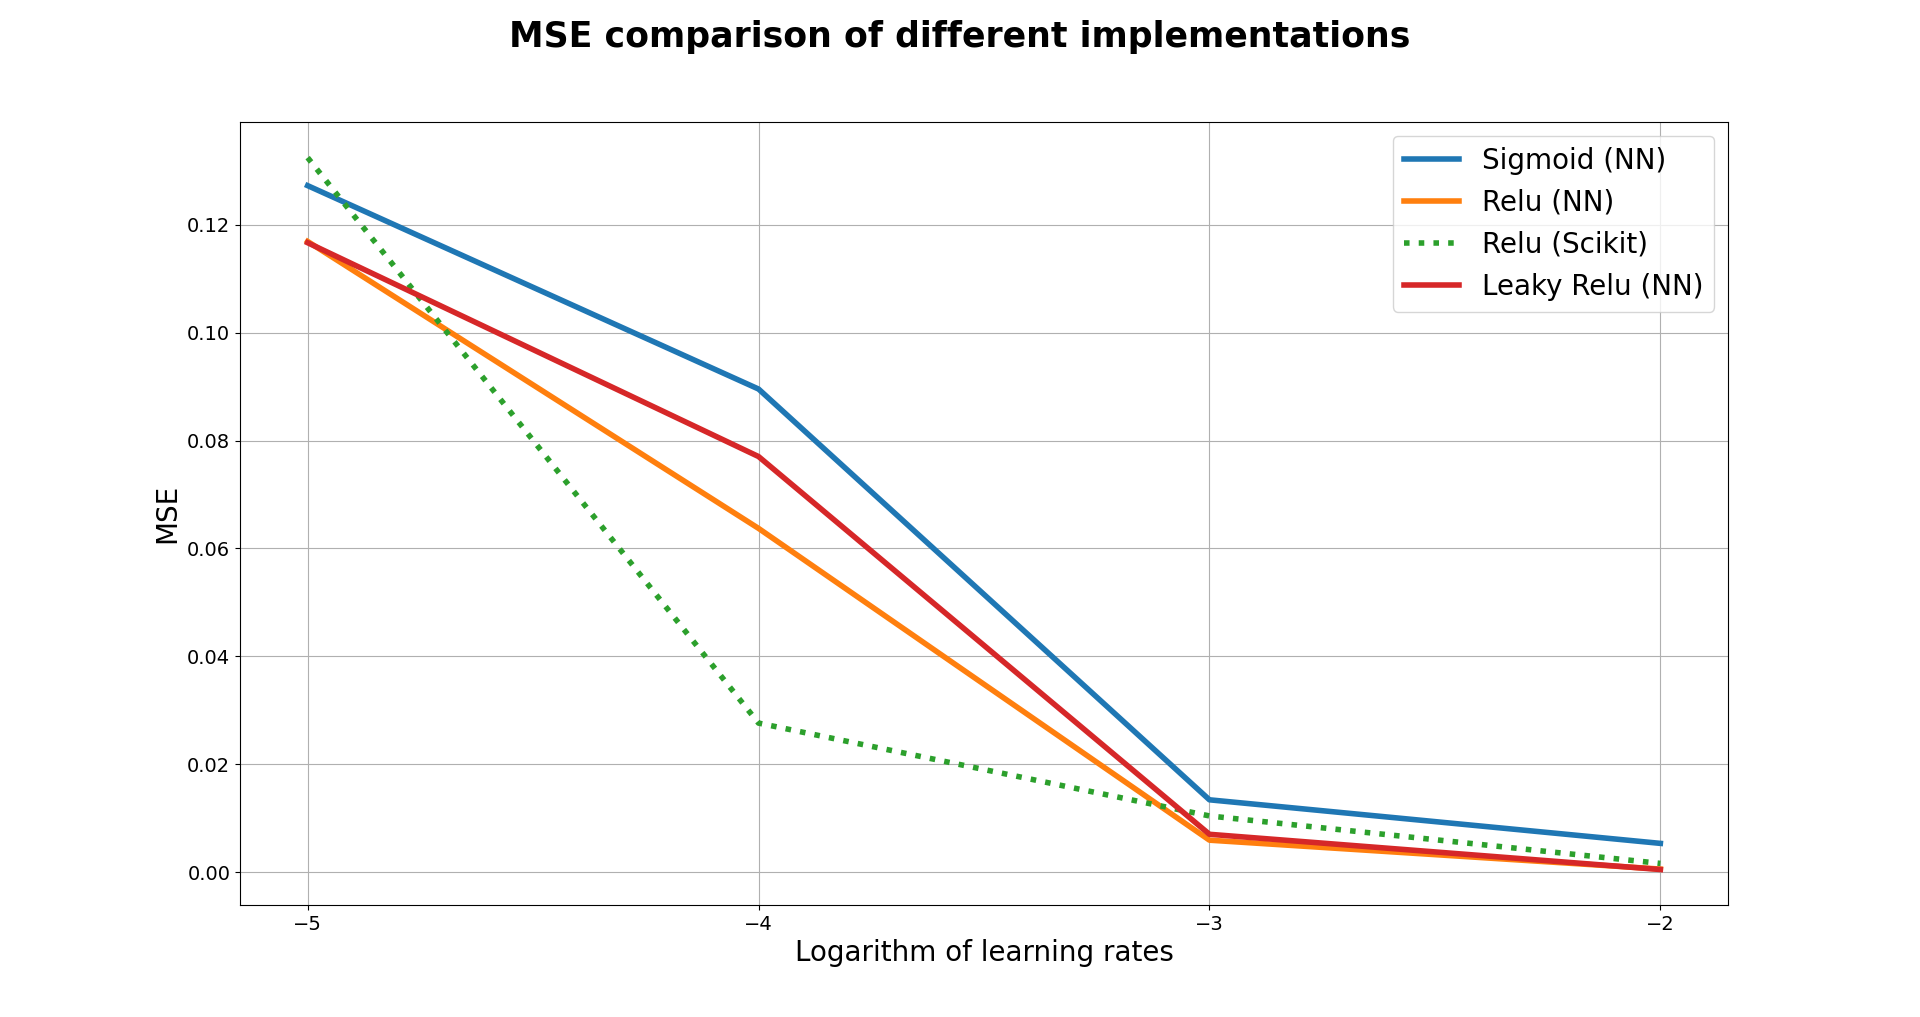
\includegraphics[width = 1\linewidth]{C:/Users/Sander/Documents/GitHub/FYS-STK4155/Project2/Project2/Report/Figures/MSEvsLearn_OLS_TOTAL_epoch2000_batch10.PNG}
\caption{\label{fig:MSEvsLrateTOTAL5} The MSE as function of number of learning rate for the three activation functions when we utilize 2000 epoch iterations and a batch size of 10. This is the OLS equivalent.}
\end{figure}

\begin{figure}[H]
\centering
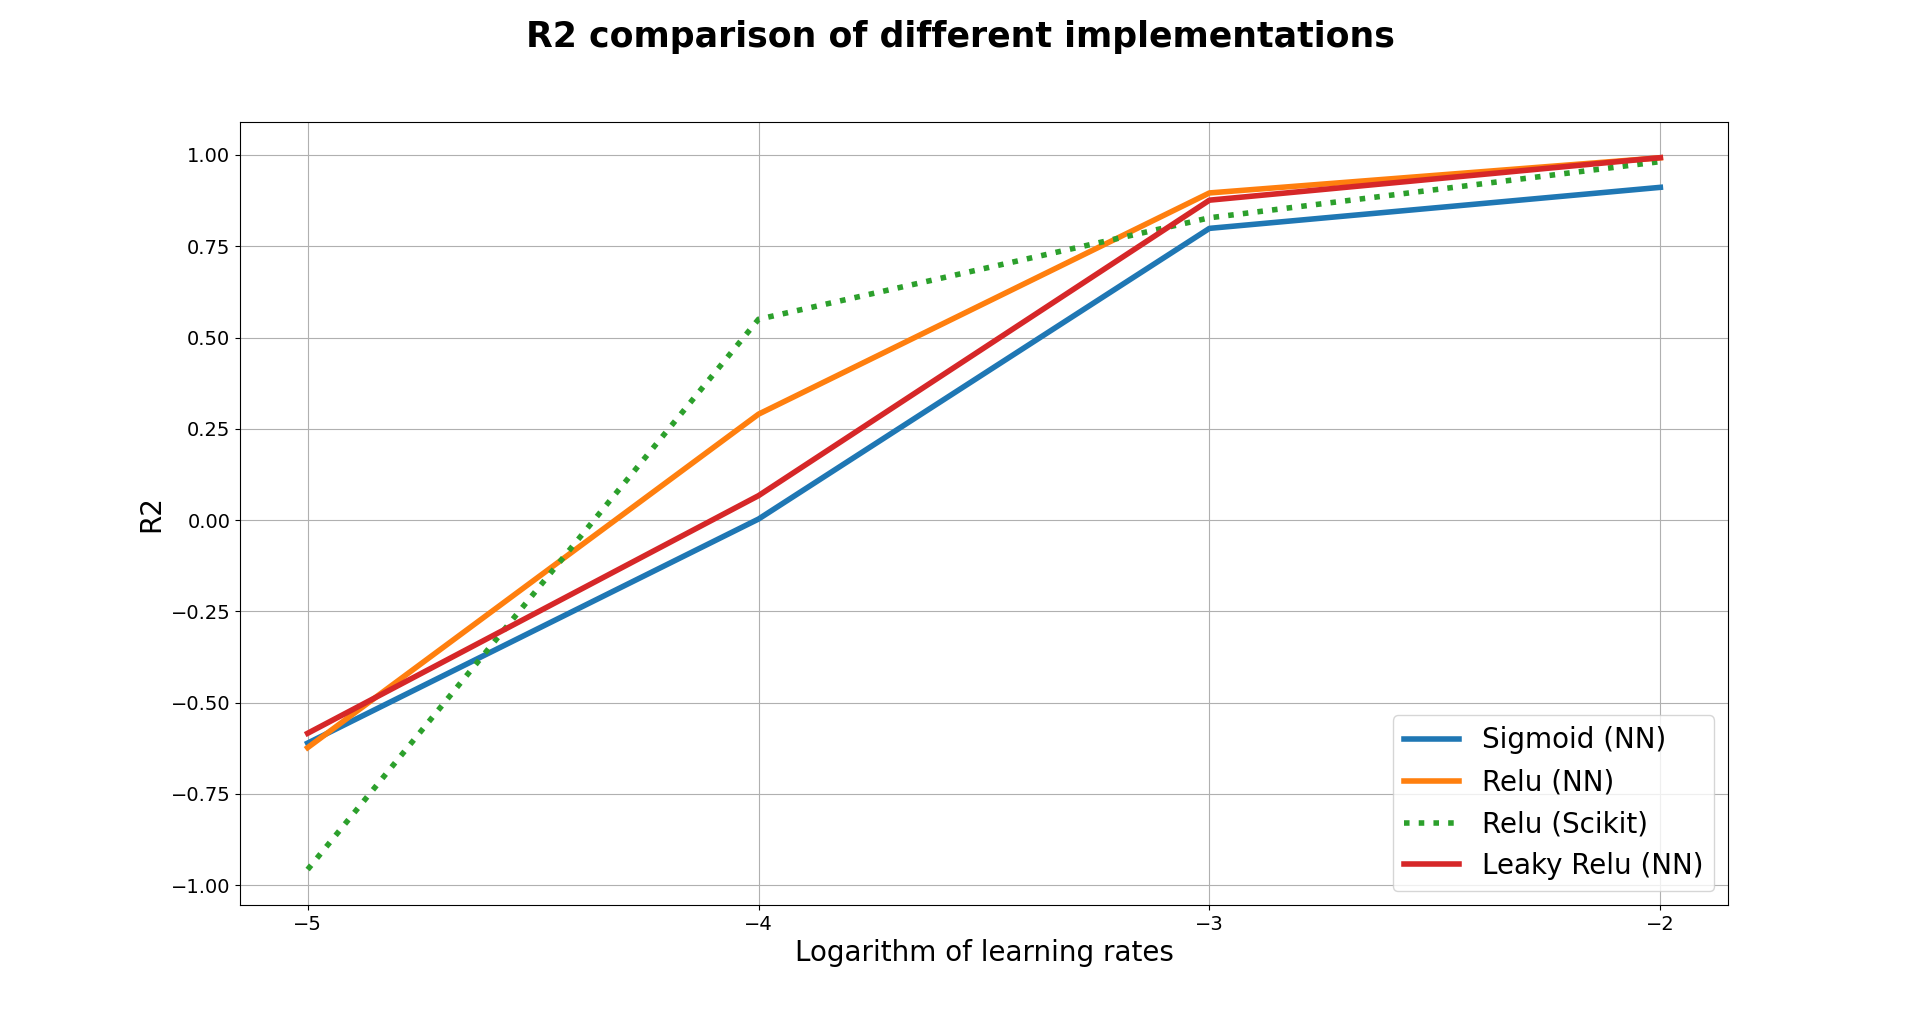
\includegraphics[width = 1\linewidth]{C:/Users/Sander/Documents/GitHub/FYS-STK4155/Project2/Project2/Report/Figures/MSEvsLearn_OLS_TOTAL_epoch2000_batch10_r2.PNG}
\caption{\label{fig:MSEvsLrateTOTAL6} The $R^2$ as function of number of learning rate for the three activation functions when we utilize 2000 epoch iterations and a batch size of 10. This is the OLS equivalent.}
\end{figure}

\noindent One can observe from figures \ref{fig:MSEvsLrateTOTAL5} and \ref{fig:MSEvsLrateTOTAL6} that the three implementations now perform about the same. This leads one to believe that there is a given threshold for when the activation functions are equivalent. At learning rates higher than 0.001, my implementations performs on par with the Scikit implementation, which is reassuring. 
\\
We now aim to see the variation in term of the size of the batch. We keep the number of epochs at 2000, but decrease the batch size from 10 to 2. Figures QQQ and QQQ shows these results.

\begin{figure}[H]
\centering
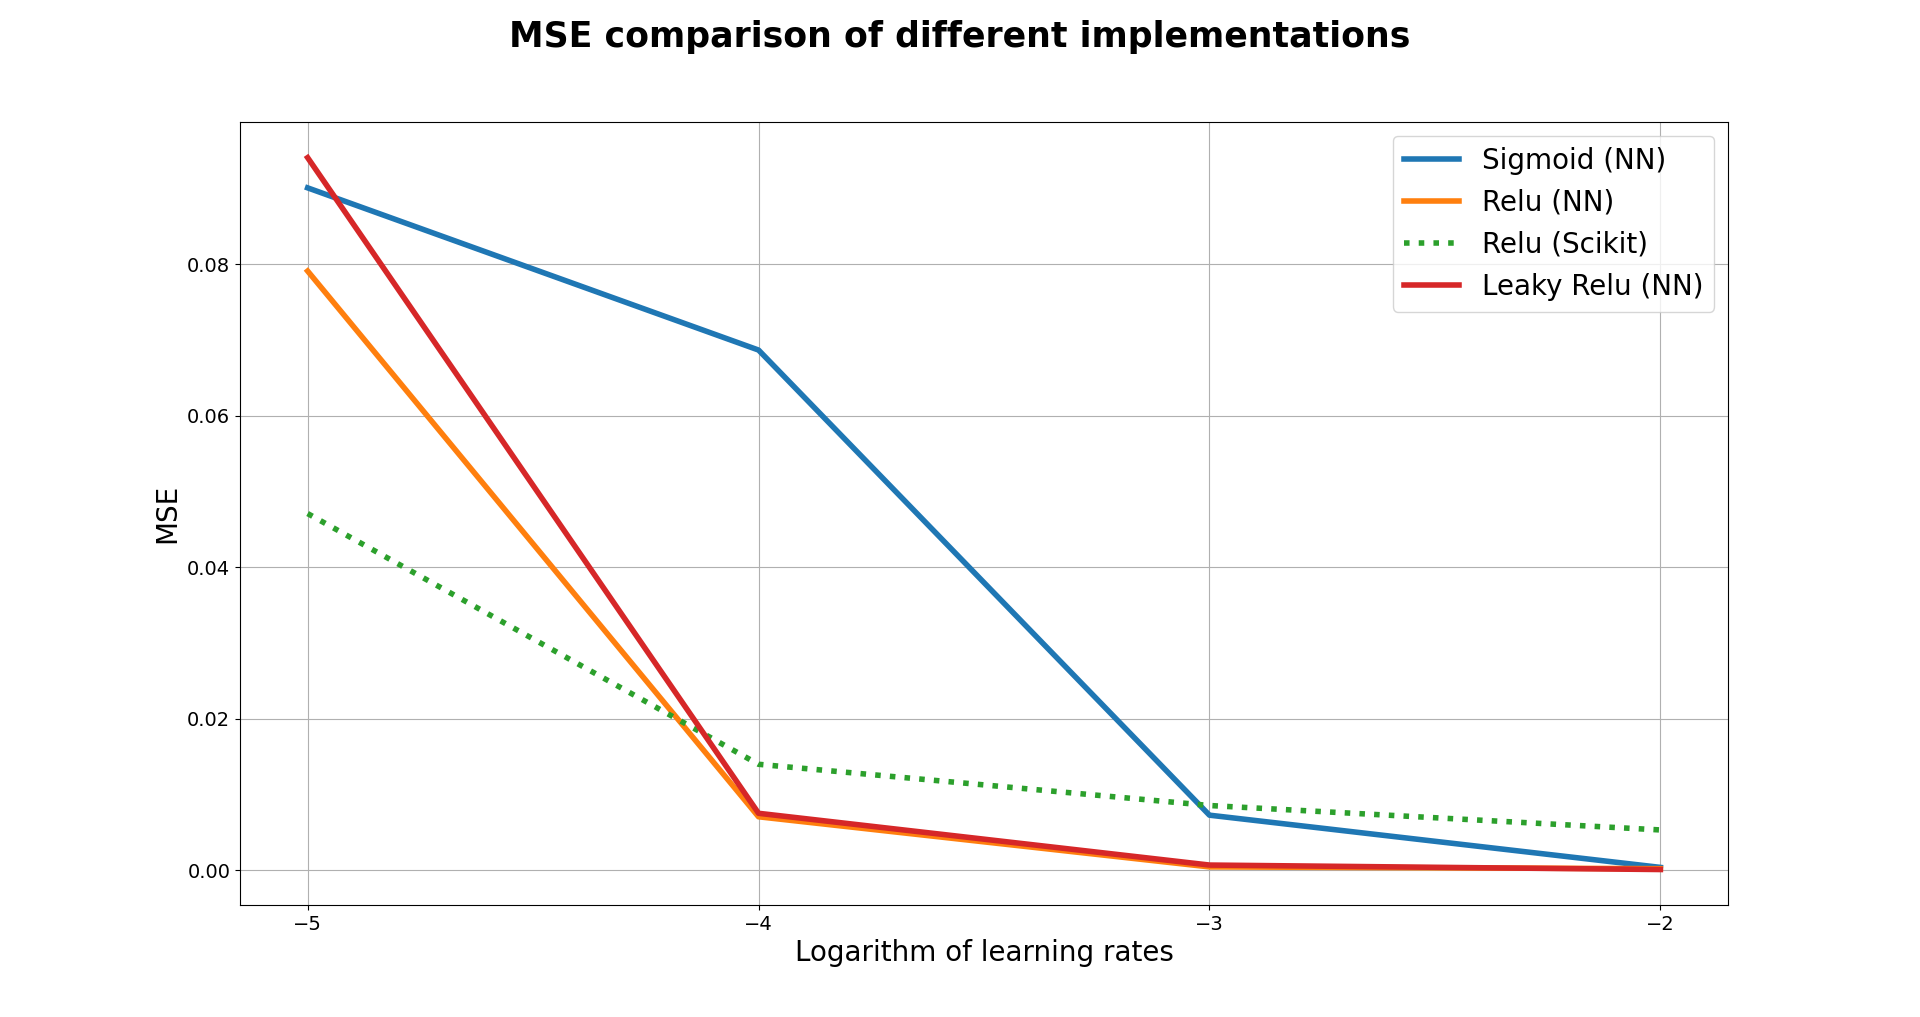
\includegraphics[width = 1\linewidth]{C:/Users/Sander/Documents/GitHub/FYS-STK4155/Project2/Project2/Report/Figures/MSEvsLearn_OLS_TOTAL_epoch2000_batch2.PNG}
\caption{\label{fig:MSEvsLrateTOTAL7} The MSE as function of number of learning rate for the three activation functions when we utilize 2000 epoch iterations and a batch size of 2. This is the OLS equivalent.}
\end{figure}

\begin{figure}[H]
\centering
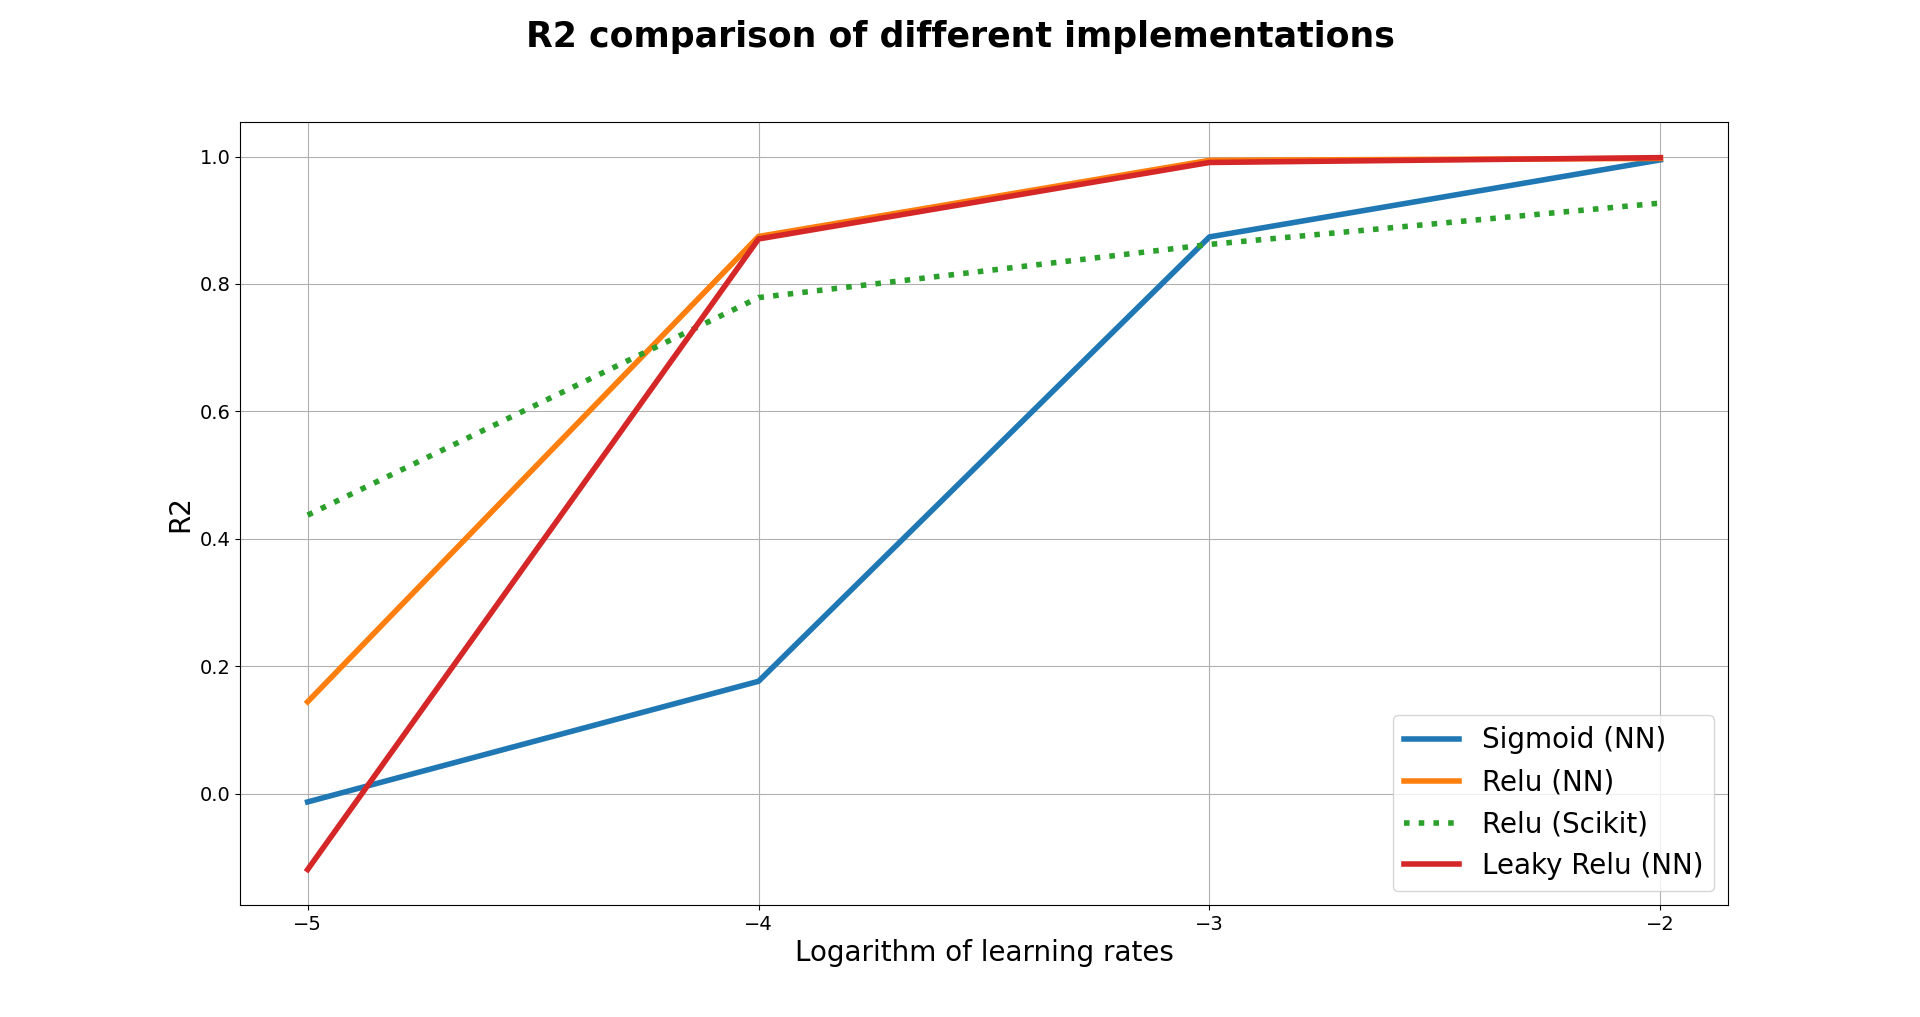
\includegraphics[width = 1\linewidth]{C:/Users/Sander/Documents/GitHub/FYS-STK4155/Project2/Project2/Report/Figures/MSEvsLearn_OLS_TOTAL_epoch2000_batch2_r2.PNG}
\caption{\label{fig:MSEvsLrateTOTAL8} The $R^2$ as function of number of learning rate for the three activation functions when we utilize 2000 epoch iterations and a batch size of 2. This is the OLS equivalent.}
\end{figure}

\noindent One can observe that the decreasing the batch size does not really impact the Scikit and sigmoid implementations, but the RELU implementations are severely improved. In fact, the RELU implementations outperform the Scikit implementations at learning rates over 0.0001. Additionally, my own implementations outperform the Scikit implementations for learning rates higher than 0.001.
\\
We now see that increasing the number of epoch and decreasing the batch size leads to better prediction for my own neural network implementations. The next goal is to find the number of hidden layers and hidden neurons that minimize the MSE (or maximize the $R^2$). To do this, we implement the different activation functions using 2000 epoch iterations and a batch size of 2. Then, we can plot a heatmap where we study the MSE as function of the number of hidden layers and hidden neurons. We only consider hidden layers between 1 and 10 and hidden neurons between 1 and 100, as this task is extremely computationally heavy using 2000 epoch iterations and a batch size of 2. The MSE heatmap using the sigmoid activation function can be seen in figure \ref{fig:heatmap1}

\begin{figure}[H]
\centering
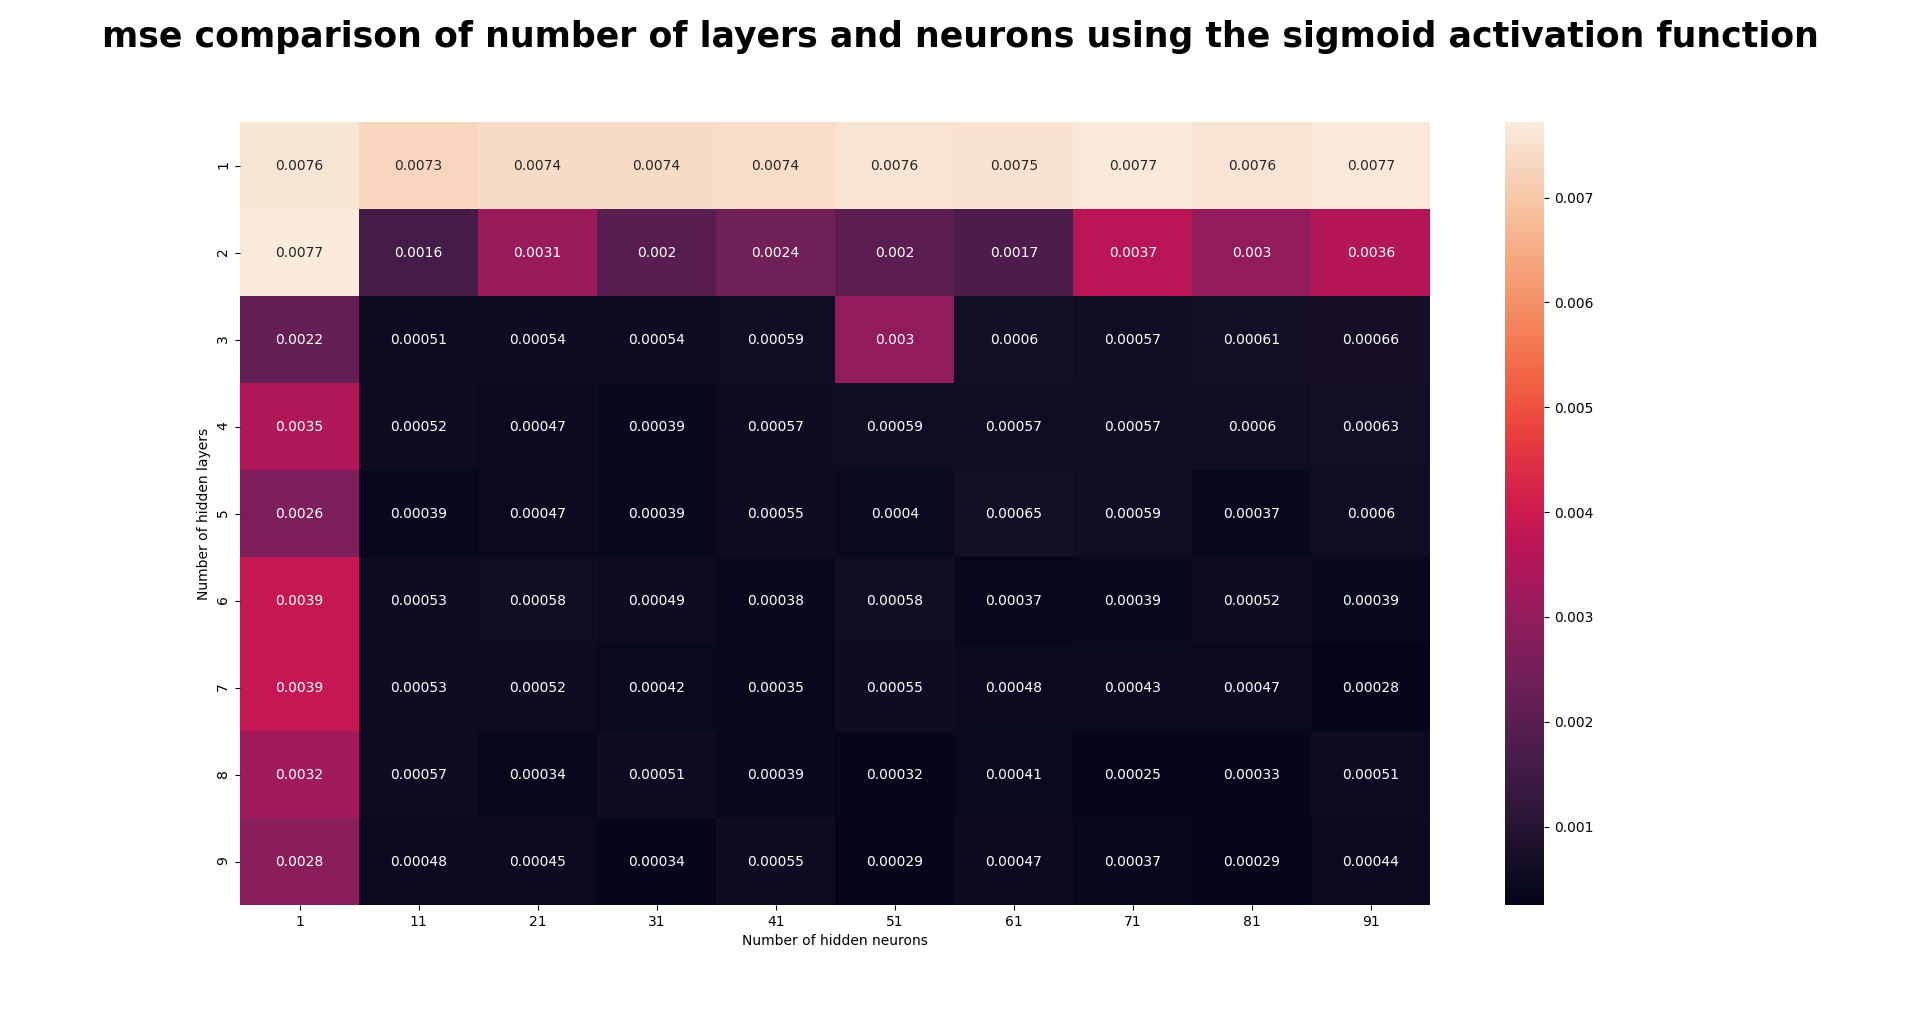
\includegraphics[width = 1\linewidth]{C:/Users/Sander/Documents/GitHub/FYS-STK4155/Project2/Project2/Report/Figures/heatmapOLS_TOTAL_sigmoidMSE_REAL.PNG}
\caption{\label{fig:heatmap1} Heatmap for different number of hidden layers and neurons using the sigmoid activation function. This is the OLS equivalent.}
\end{figure}

\noindent One can observe from the heatmap in figure \ref{fig:heatmap1} that the neural network performs well as long as we keep the number of hidden layers above 4 and the number of hidden neurons above 10. In this range, the MSE is less than $0.0006$ which means the network is able to predict the Franke function accurately. Let us now take a look at the RELU implementation using both my own and the Scikit implementation as seen in figures QQQ and QQQ.

\begin{figure}[H]
\centering
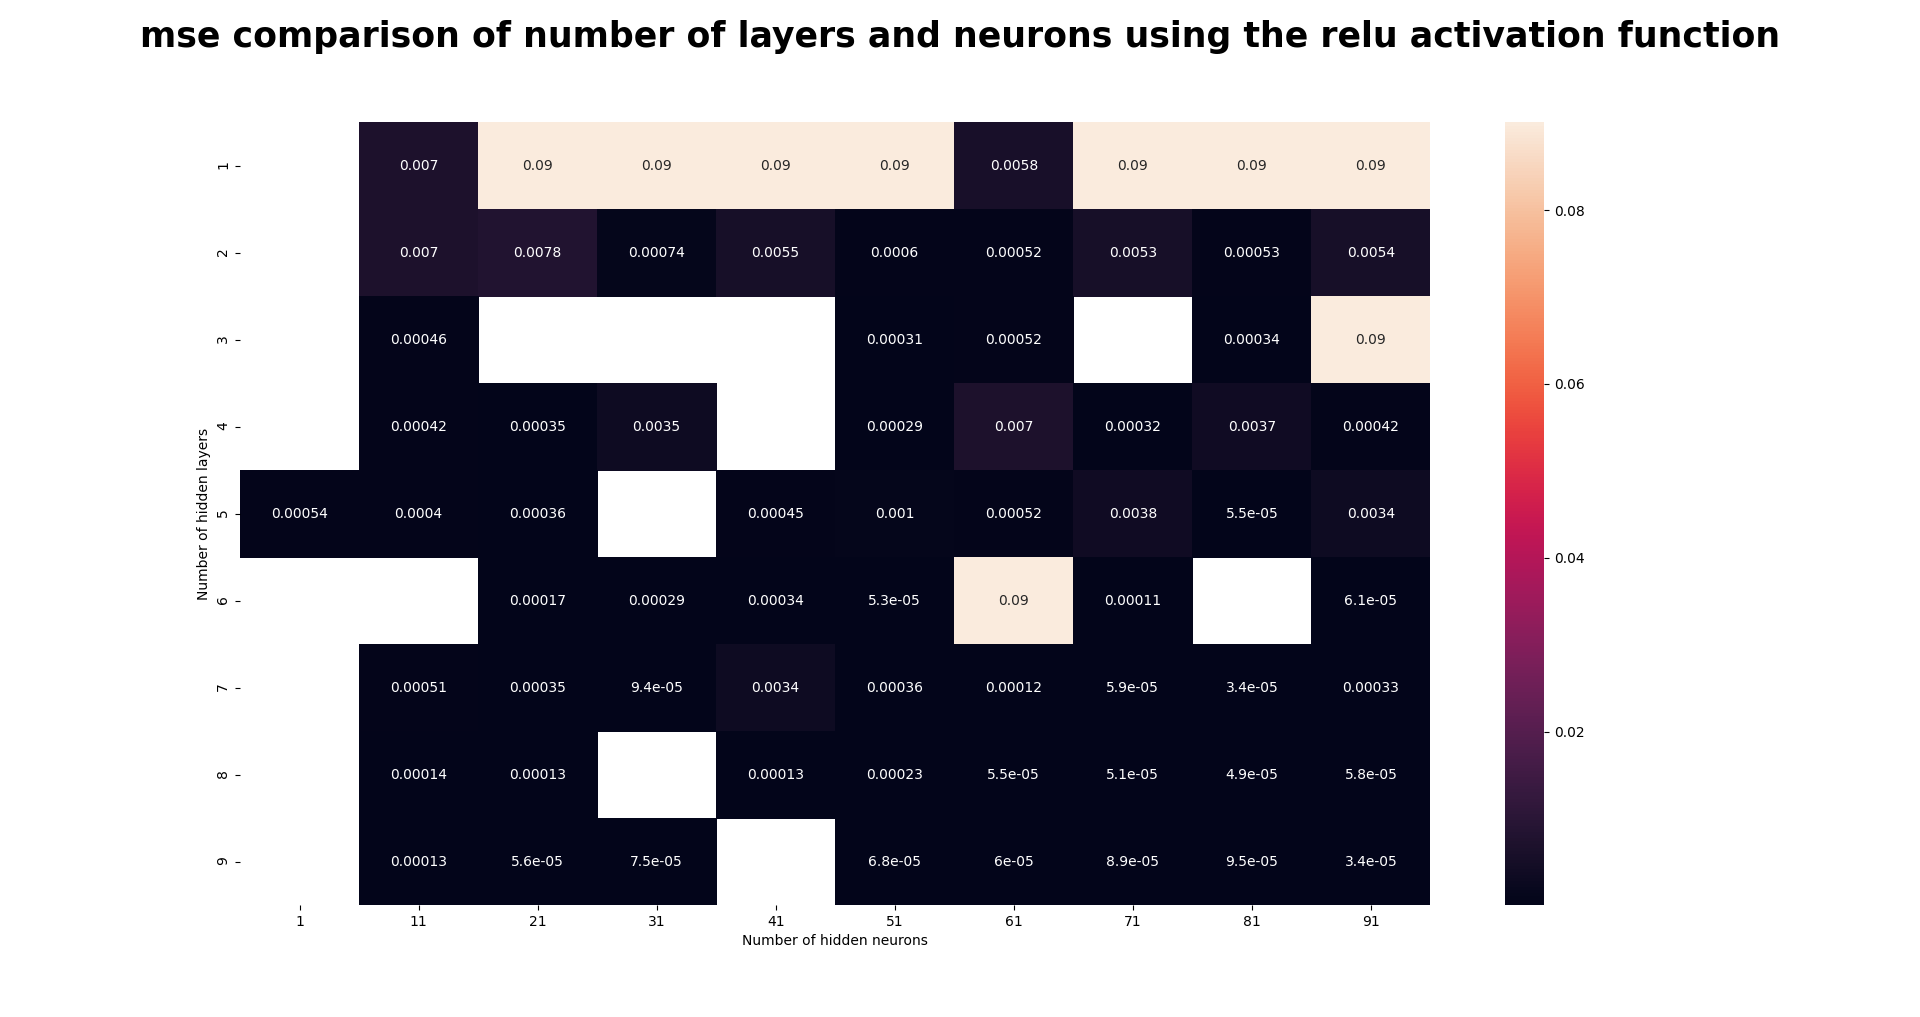
\includegraphics[width = 1\linewidth]{C:/Users/Sander/Documents/GitHub/FYS-STK4155/Project2/Project2/Report/Figures/heatmapOLS_TOTAL_reluMSE_REAL.PNG}
\caption{\label{fig:heatmap2} Heatmap for different number of hidden layers and neurons using the RELU activation function. This is the OLS equivalent.}
\end{figure}

\begin{figure}[H]
\centering
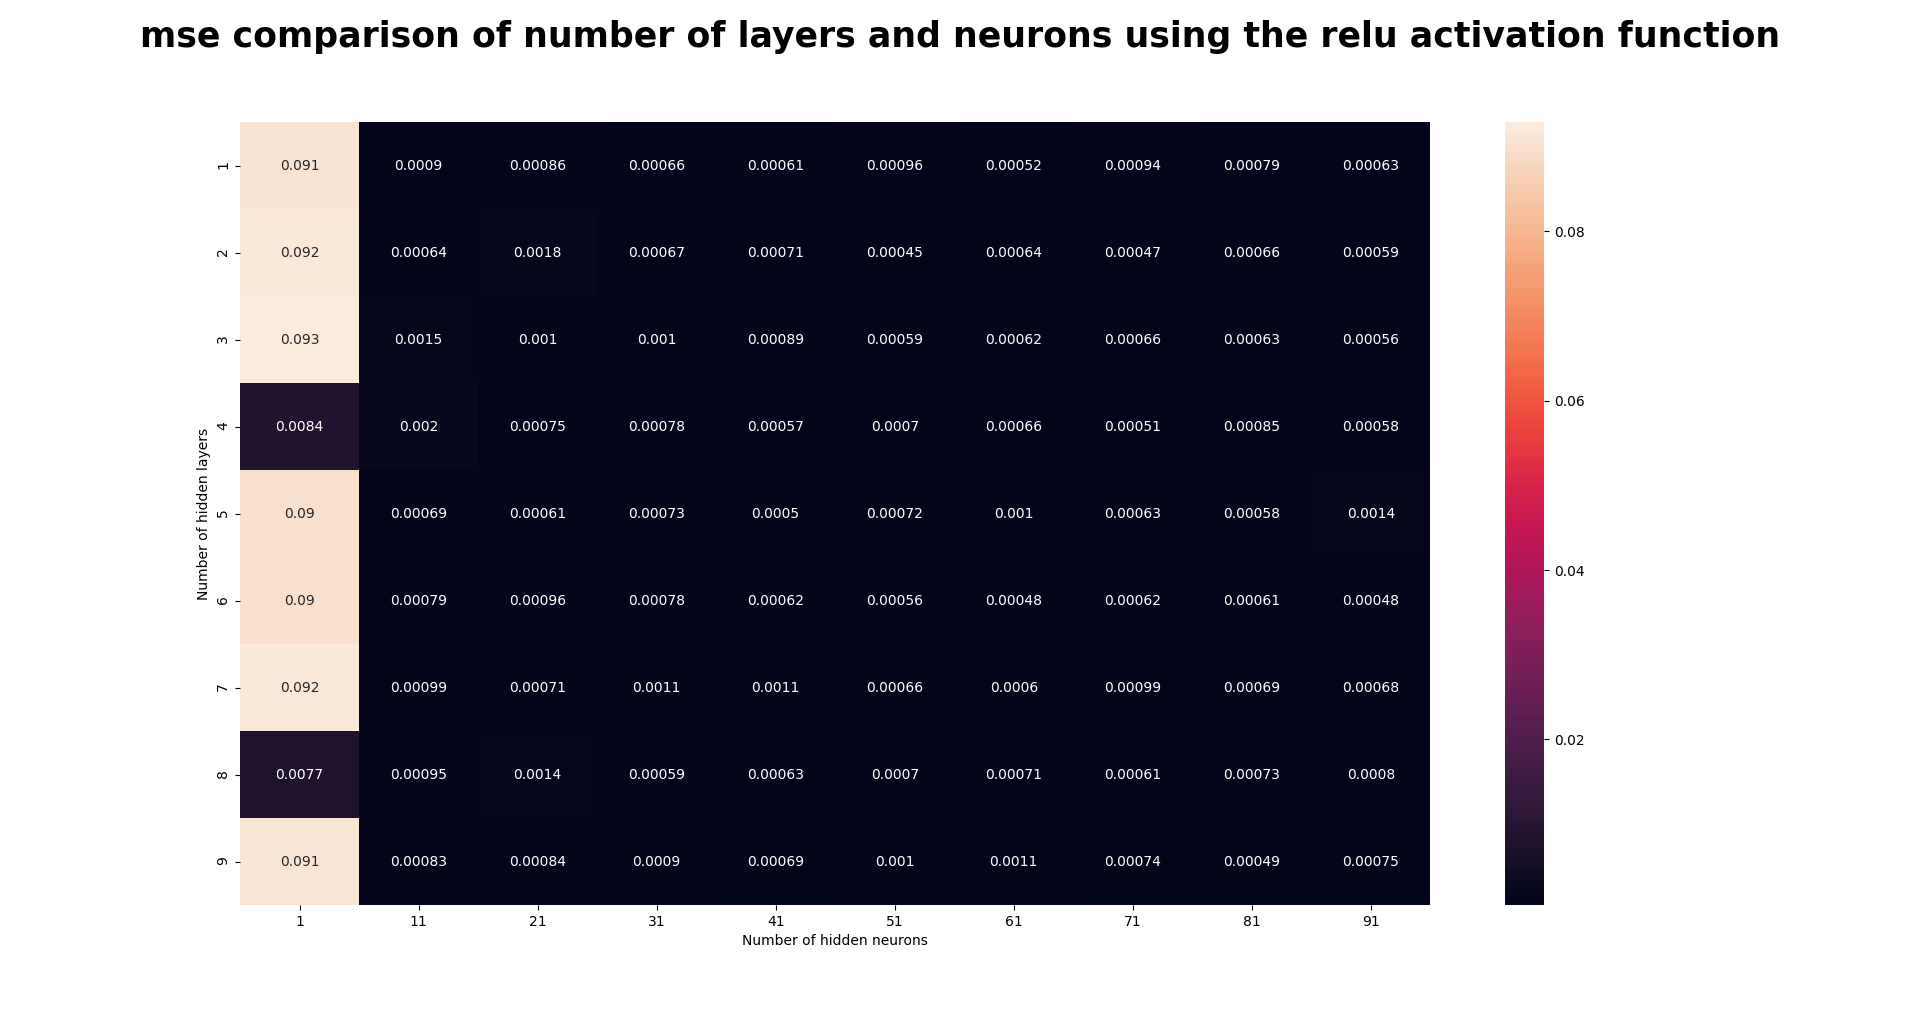
\includegraphics[width = 1\linewidth]{C:/Users/Sander/Documents/GitHub/FYS-STK4155/Project2/Project2/Report/Figures/heatmapOLS_TOTAL_reluMSE_sci_REAL.PNG}
\caption{\label{fig:heatmap3} Heatmap for different number of hidden layers and neurons using the RELU activation function with the Scikit implementation. This is the OLS equivalent.}
\end{figure}

\noindent One can observe from figure \ref{fig:heatmap2} that my own network experienced overflow at given layer/neuron configurations, as some of the squares in the heatmap is not included. This is particularly the case when there is only 1 hidden neuron in the layers. However, the network seems stable for a larger number of neurons in the layers. For hidden neurons above 30 and hidden layers above 5 it can be observed from figure \ref{fig:heatmap2} that the network is able to produce MSEs of under $0.0003$ which is lower than that of the sigmoid implementation. The Scikit implementation seems to be stable at any and all configurations of hidden layers and neurons. However, when there is only 1 neuron per hidden layer, the network gives a really high MSE. It is likely that the Scikit package includes some anti-overflow procedures that makes the algorithm able to deal with the overflow, but the neuron/layer configuration here still yields terrible results. We also observe that the MSE of the Scikit implementation is lower than that of my own implementation. These observations are compatable with those observed in figures \ref{fig:MSEvsLrateTOTAL1} to \ref{fig:MSEvsLrateTOTAL8}. 
\\
The leaky RELU implementation is plotted in figure \ref{fig:heatmap4}

\begin{figure}[H]
\centering
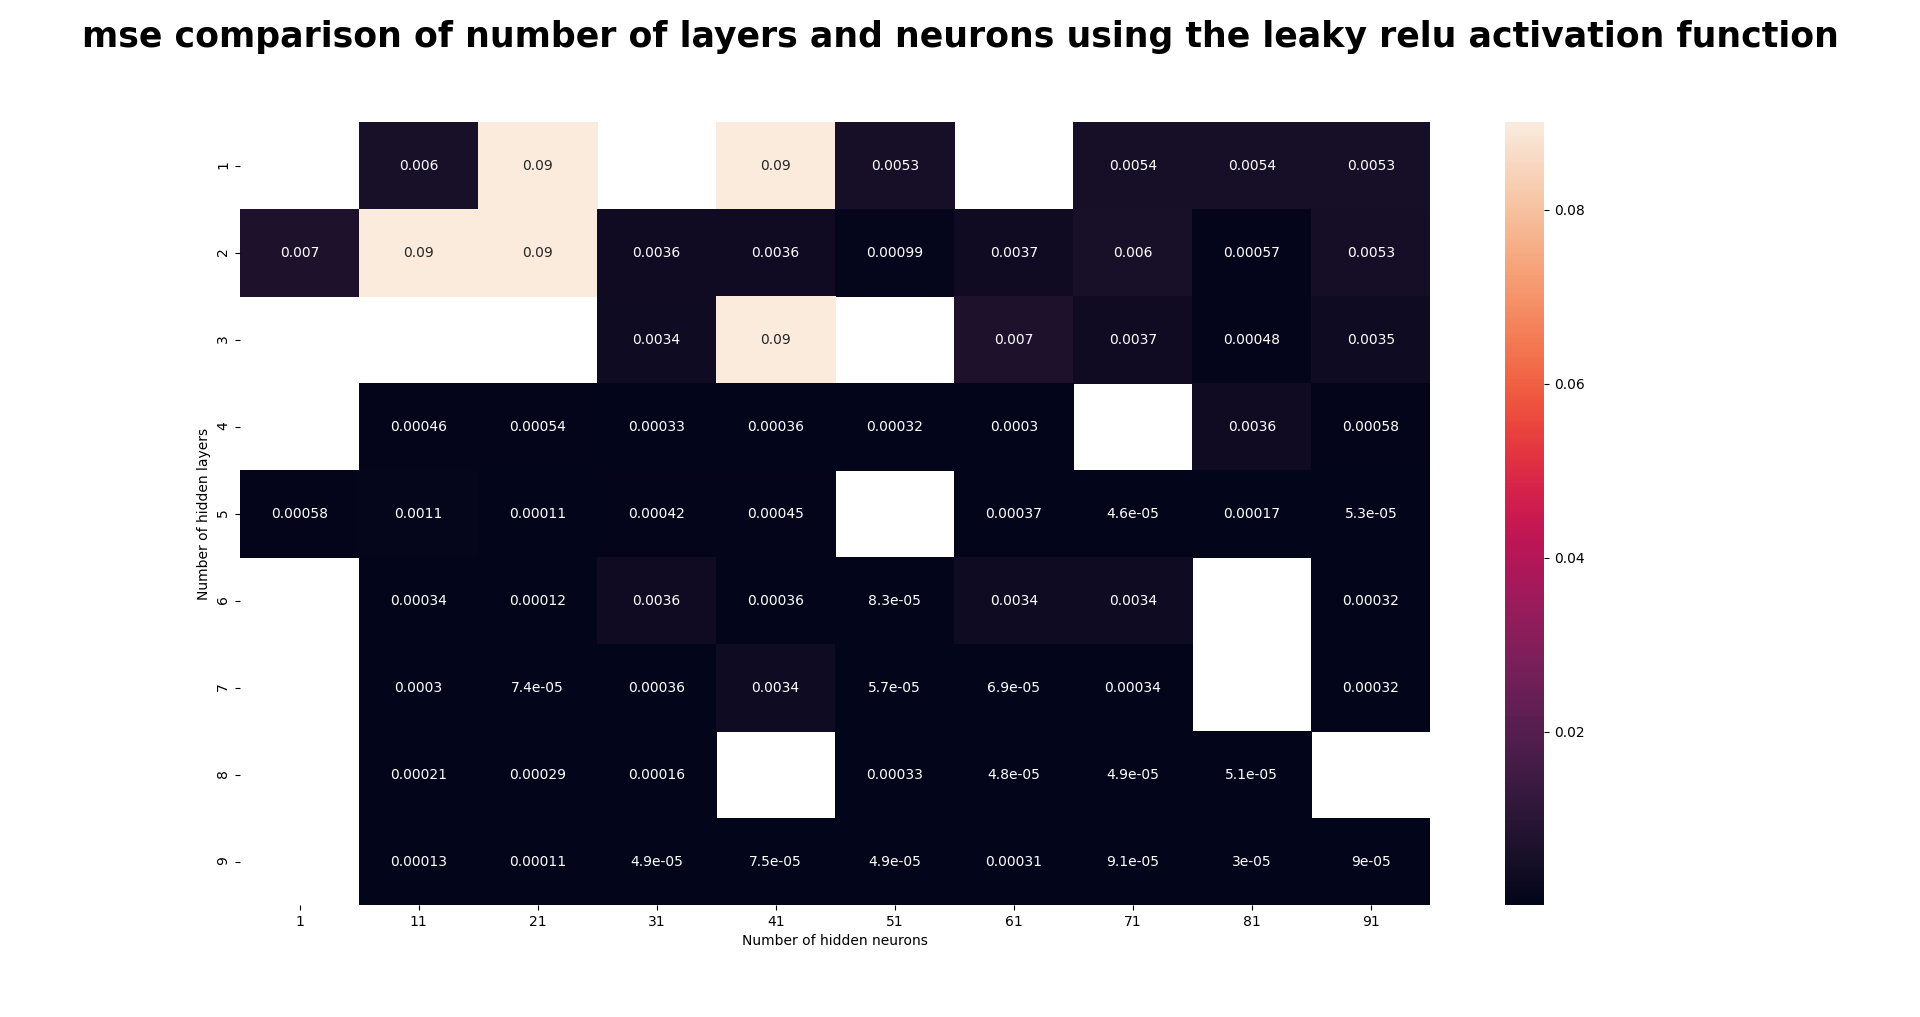
\includegraphics[width = 1\linewidth]{C:/Users/Sander/Documents/GitHub/FYS-STK4155/Project2/Project2/Report/Figures/heatmapOLS_TOTAL_leakyreluMSE_REAL.PNG}
\caption{\label{fig:heatmap4} Heatmap for different number of hidden layers and neurons using the leaky RELU activation function with the Scikit implementation. This is the OLS equivalent.}
\end{figure}

\noindent One can observe from figure \ref{fig:heatmap4} that it resembles my own RELU implementation seen in figure \ref{fig:heatmap2}. However, the algorithms is more unstable and there are many overflows occurring even for more layers and neurons. However, the MSE in the leaky RELU implementation seems to yield similar MSE values to the RELU implementation (slightly higher).

\begin{center}
\large{\textbf{Ridge equivalent implementation}}
\end{center}

\noindent We now aim to perform the above analysis, but using the Ridge equivalent implementation. The Ridge implementation works similar to that of linear regression, but we here add the penalty parameter while the neural network performs the back propagation so that the penalty is applied to the hidden weights within the network (kilde). The weights are then adjusted with the penalty parameter in mind and the result is a reduction in what weights contribute to the overall output of the network. The penalty parameter was in this case set to $0.001$ as this was seen to yield good results in the previous project. 
\\
We can begin the analysis by plotting the MSE and $R^2$ as function of the learning rate for the sigmoid, RELU (both Scikit and mine) and leaky RELU implementations as seen in figures \ref{fig:MSEvsLrateTOTAL8} and \ref{fig:MSEvsLrateTOTAL9}.

\begin{figure}[H]
\centering
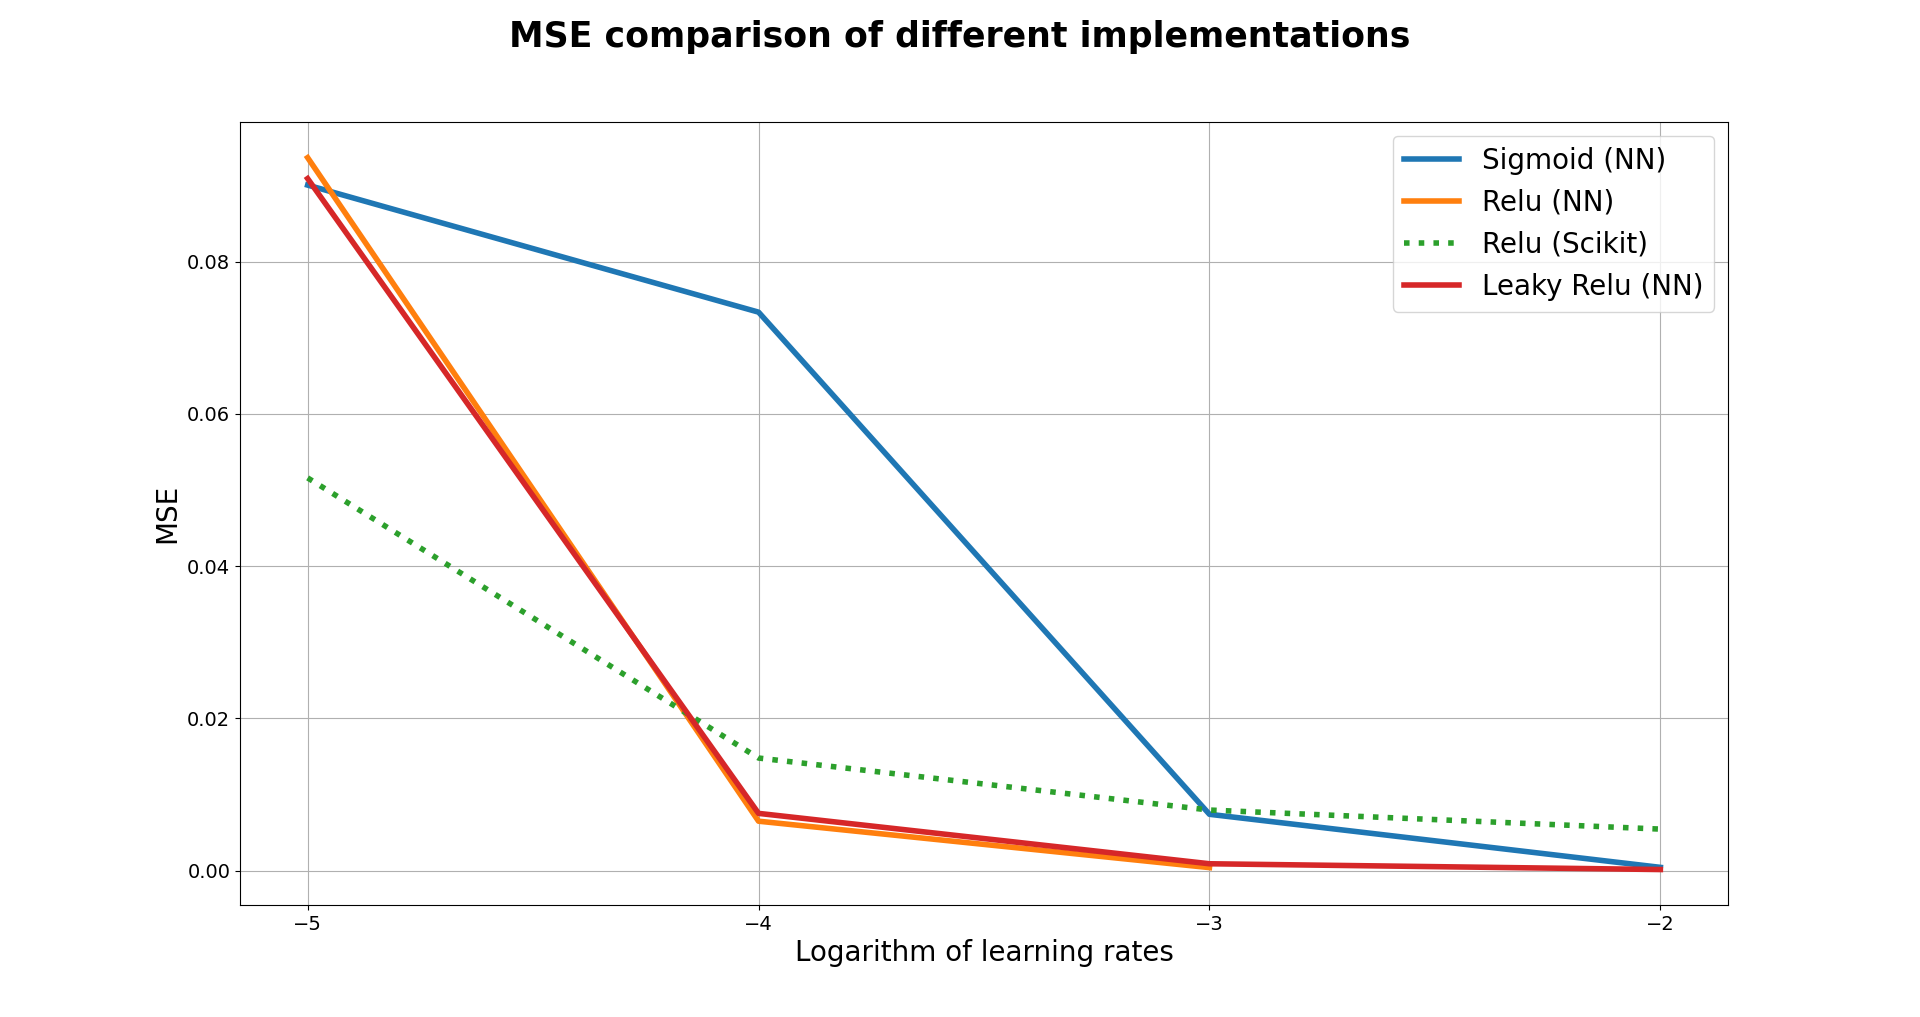
\includegraphics[width = 1\linewidth]{C:/Users/Sander/Documents/GitHub/FYS-STK4155/Project2/Project2/Report/Figures/MSEvsLearn_Ridge_TOTAL_epoch2000_batch2.PNG}
\caption{\label{fig:MSEvsLrateTOTAL8} The MSE as function of number of learning rate for the three activation functions when we utilize 2000 epoch iterations and a batch size of 2. This is the Ridge equivalent.}
\end{figure}

\begin{figure}[H]
\centering
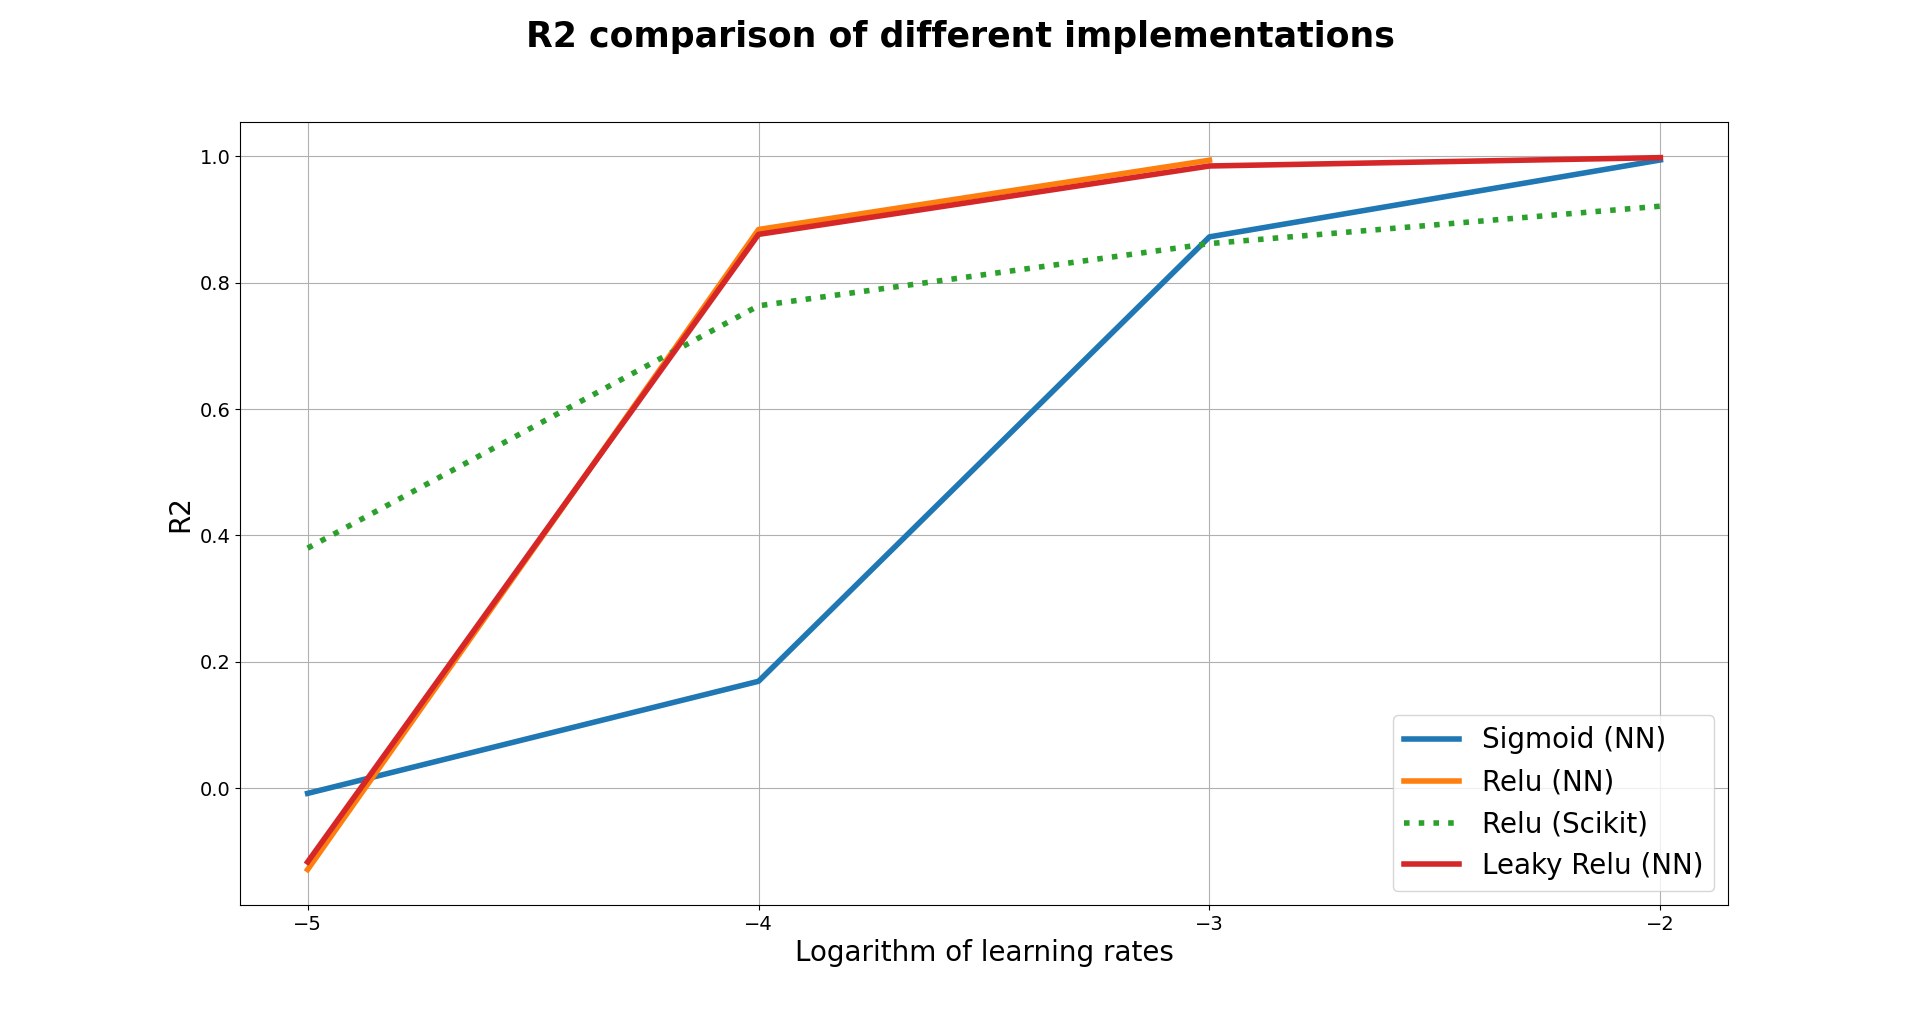
\includegraphics[width = 1\linewidth]{C:/Users/Sander/Documents/GitHub/FYS-STK4155/Project2/Project2/Report/Figures/MSEvsLearn_Ridge_TOTAL_epoch2000_batch2_r2.PNG}
\caption{\label{fig:MSEvsLrateTOTAL9} The $R^2$ as function of number of learning rate for the three activation functions when we utilize 2000 epoch iterations and a batch size of 2. This is the Ridge equivalent.}
\end{figure}

\noindent It can be observed from figures \ref{fig:MSEvsLrateTOTAL8} that the RELU and leaky RELU implementation are pretty similar both in terms of MSE and $R^2$. These two implementations performs better than the Scikit implementations for learning rates larger than 0.0001, but worse for learning rates lower than that. It can also be observed that the sigmoid implementation does not compare to any of the others. It is overall worse in terms of both MSE and $R^2$ for all learning rates. However, the sigmoid catches up at learning rate 0.01, but this often yielded overflow in the neural network, meaning it is an unfair comparison. The optimal learning rate which often did not result in overflow was 0.001 which will be used from now on.
\\
The next step would be to find which hidden neuron/layer configuration which yields the lowest MSE. Therefore, we consider neurons in the range 1 to 90 and layers in the range 1 to 10 and the MSE is then calculated using the sigmoid, RELU (both Scikit and mine) and leaky RELU activation functions. The result is plotted in the heatmaps of figures \ref{fig:heatmap5}, \ref{fig:heatmap6}, \ref{fig:heatmap7} and \ref{fig:heatmap8}.

\begin{figure}[H]
\centering
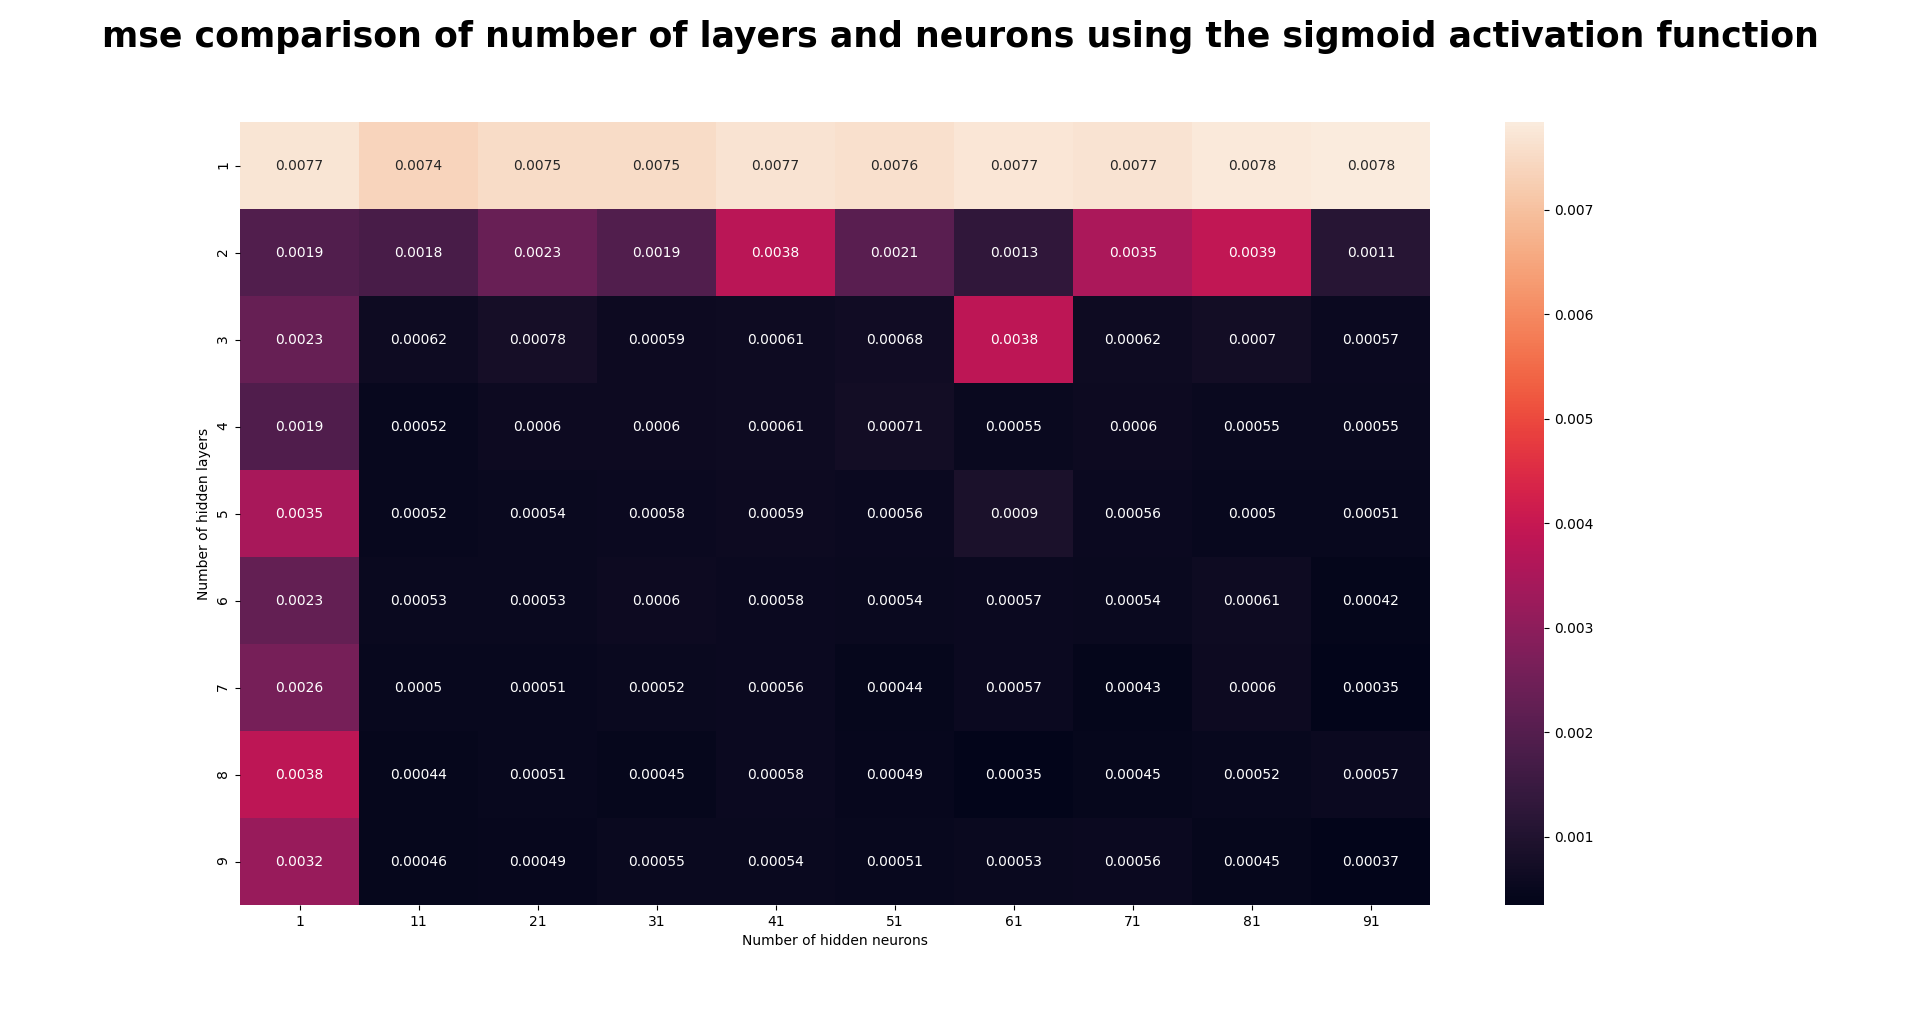
\includegraphics[width = 1\linewidth]{C:/Users/Sander/Documents/GitHub/FYS-STK4155/Project2/Project2/Report/Figures/heatmapRidge_TOTAL_sigmoid_REAL.PNG}
\caption{\label{fig:heatmap5} Heatmap for different number of hidden layers and neurons using the sigmoid activation function. This is the Ridge equivalent.}
\end{figure}

\begin{figure}[H]
\centering
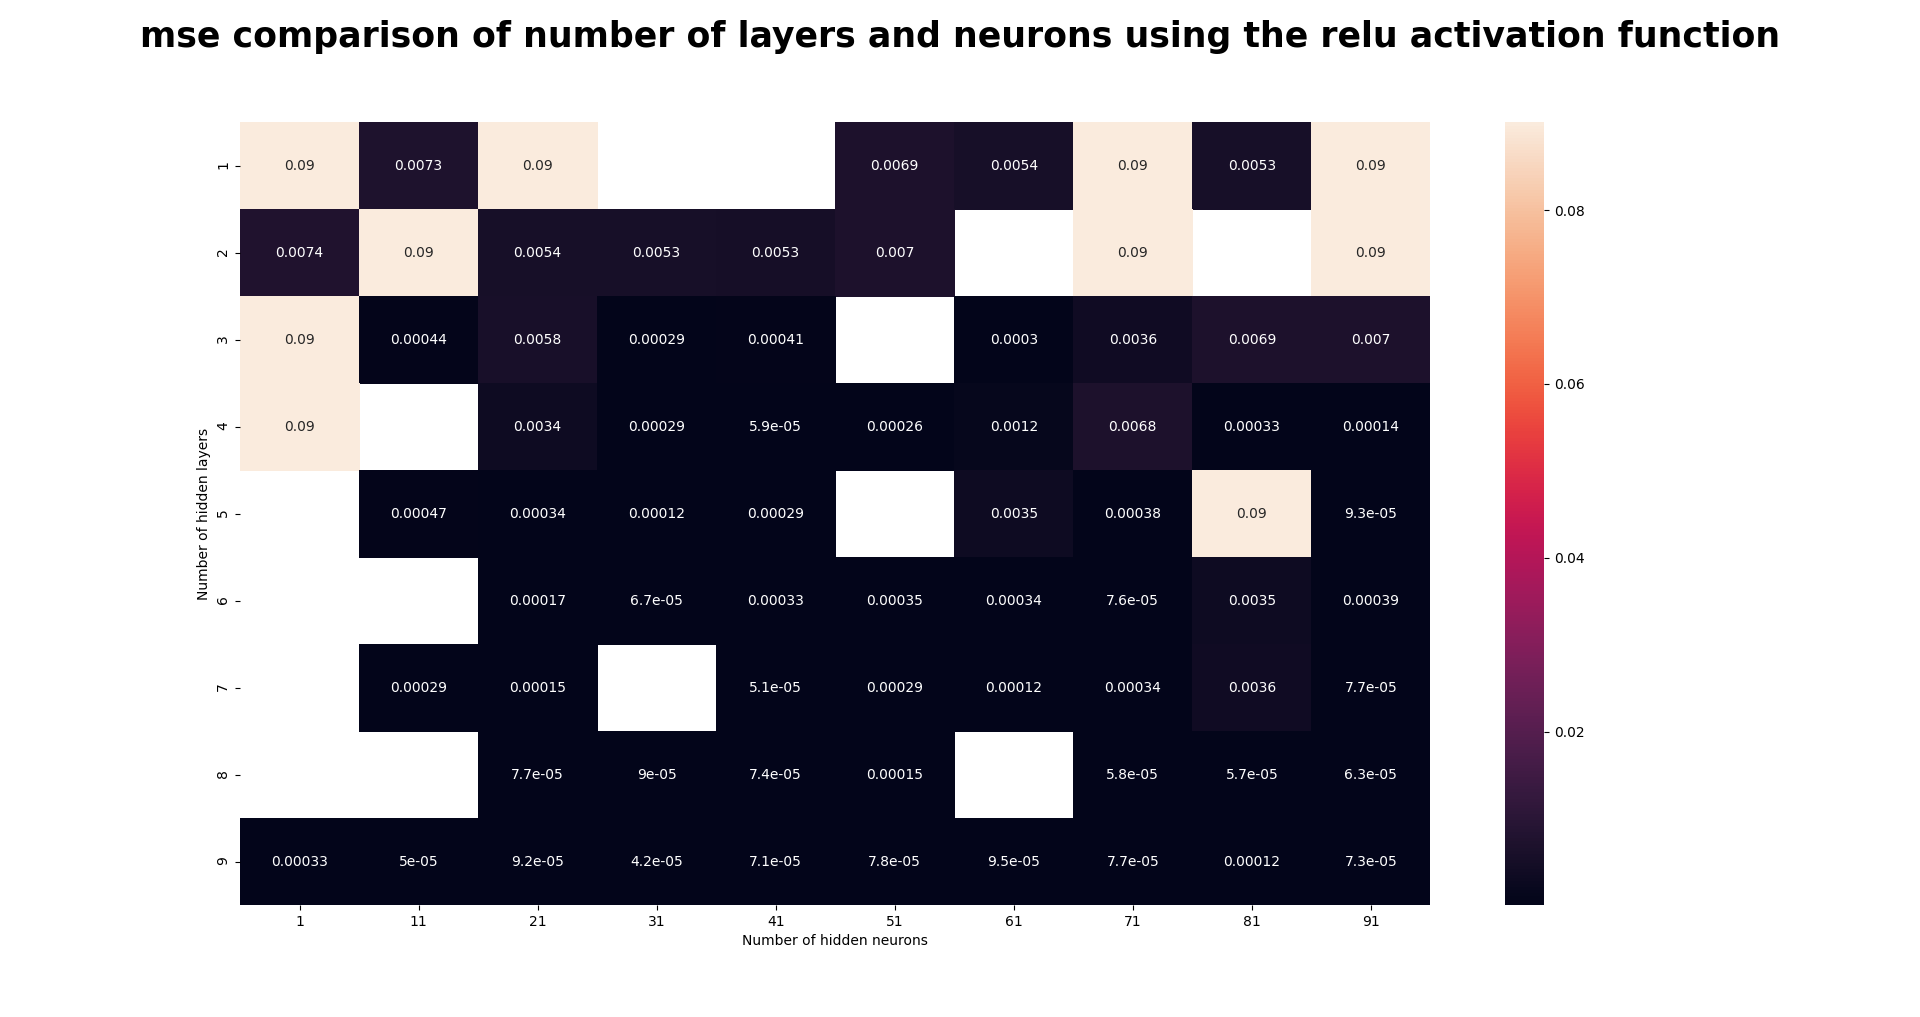
\includegraphics[width = 1\linewidth]{C:/Users/Sander/Documents/GitHub/FYS-STK4155/Project2/Project2/Report/Figures/heatmapRidge_TOTAL_relu_REAL.PNG}
\caption{\label{fig:heatmap6} Heatmap for different number of hidden layers and neurons using the RELU activation function. This is the Ridge equivalent.}
\end{figure}

\begin{figure}[H]
\centering
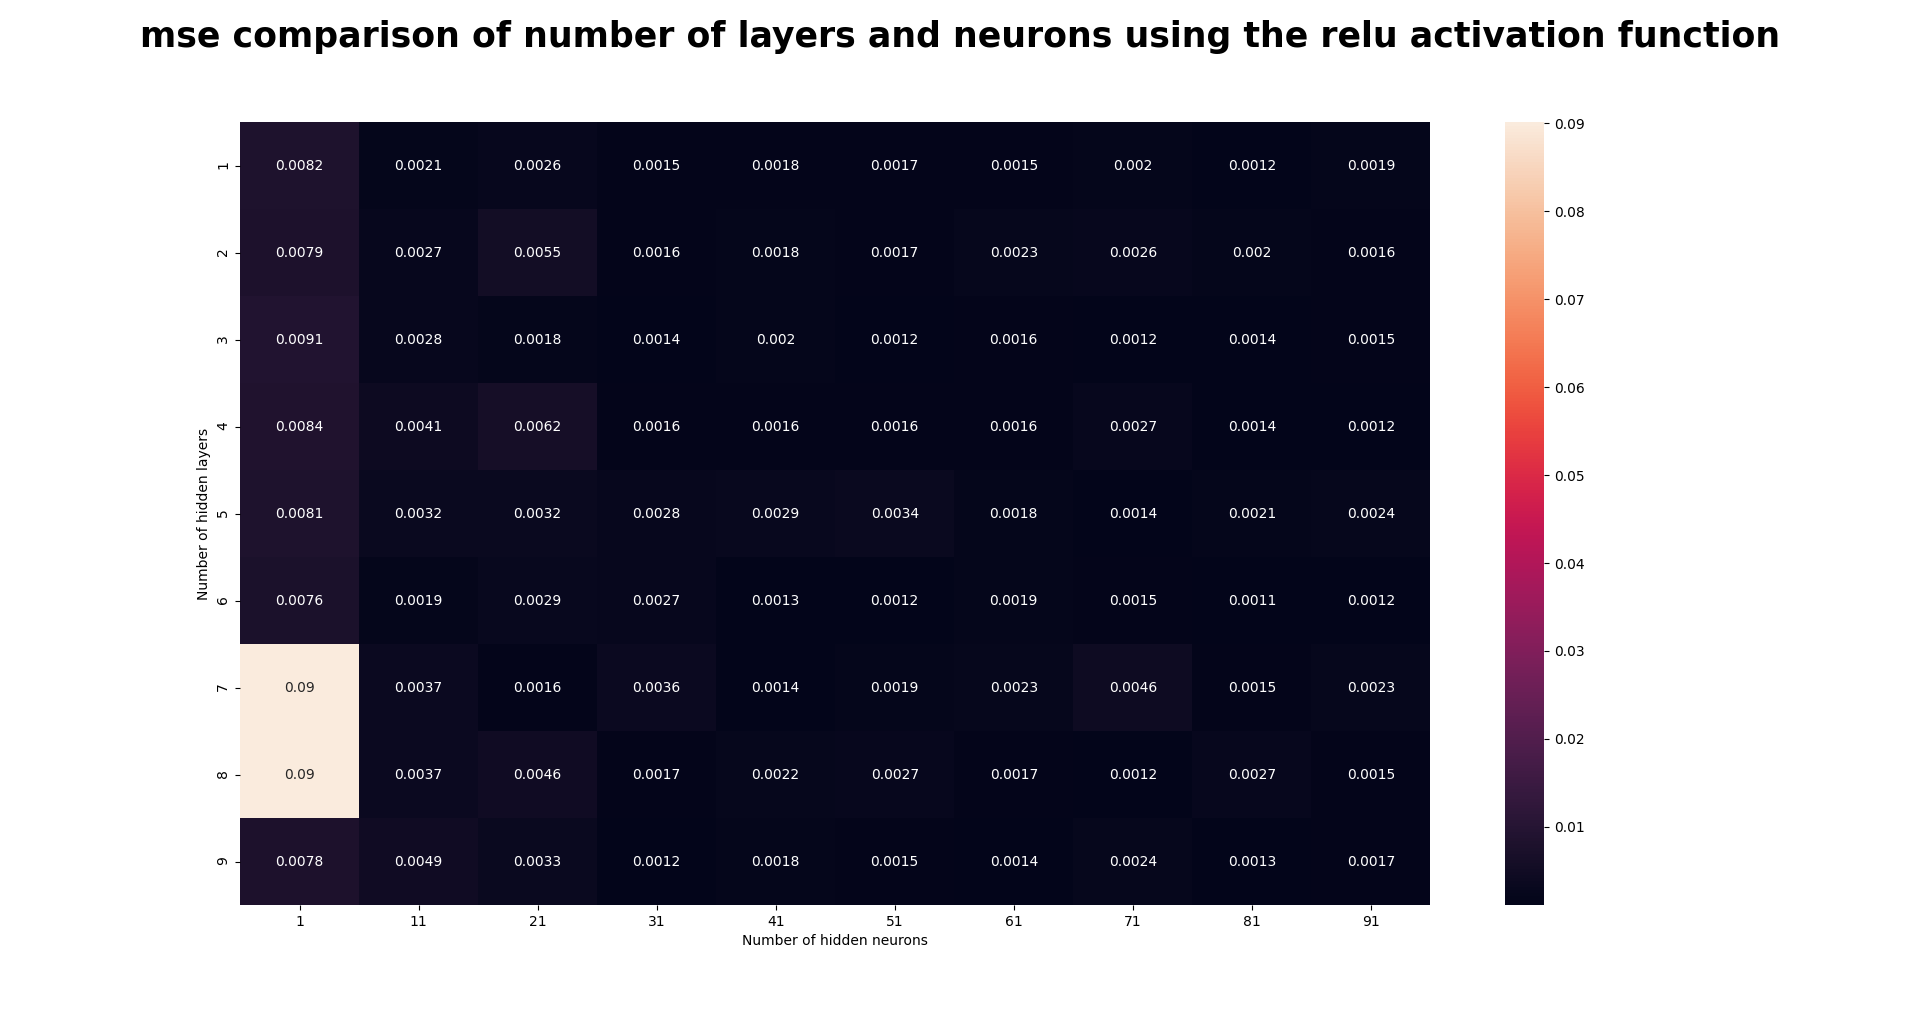
\includegraphics[width = 1\linewidth]{C:/Users/Sander/Documents/GitHub/FYS-STK4155/Project2/Project2/Report/Figures/heatmapRidge_TOTAL_relu_sci_REAL.PNG}
\caption{\label{fig:heatmap7} Heatmap for different number of hidden layers and neurons using the Scikit RELU activation function. This is the Ridge equivalent.}
\end{figure}

\begin{figure}[H]
\centering
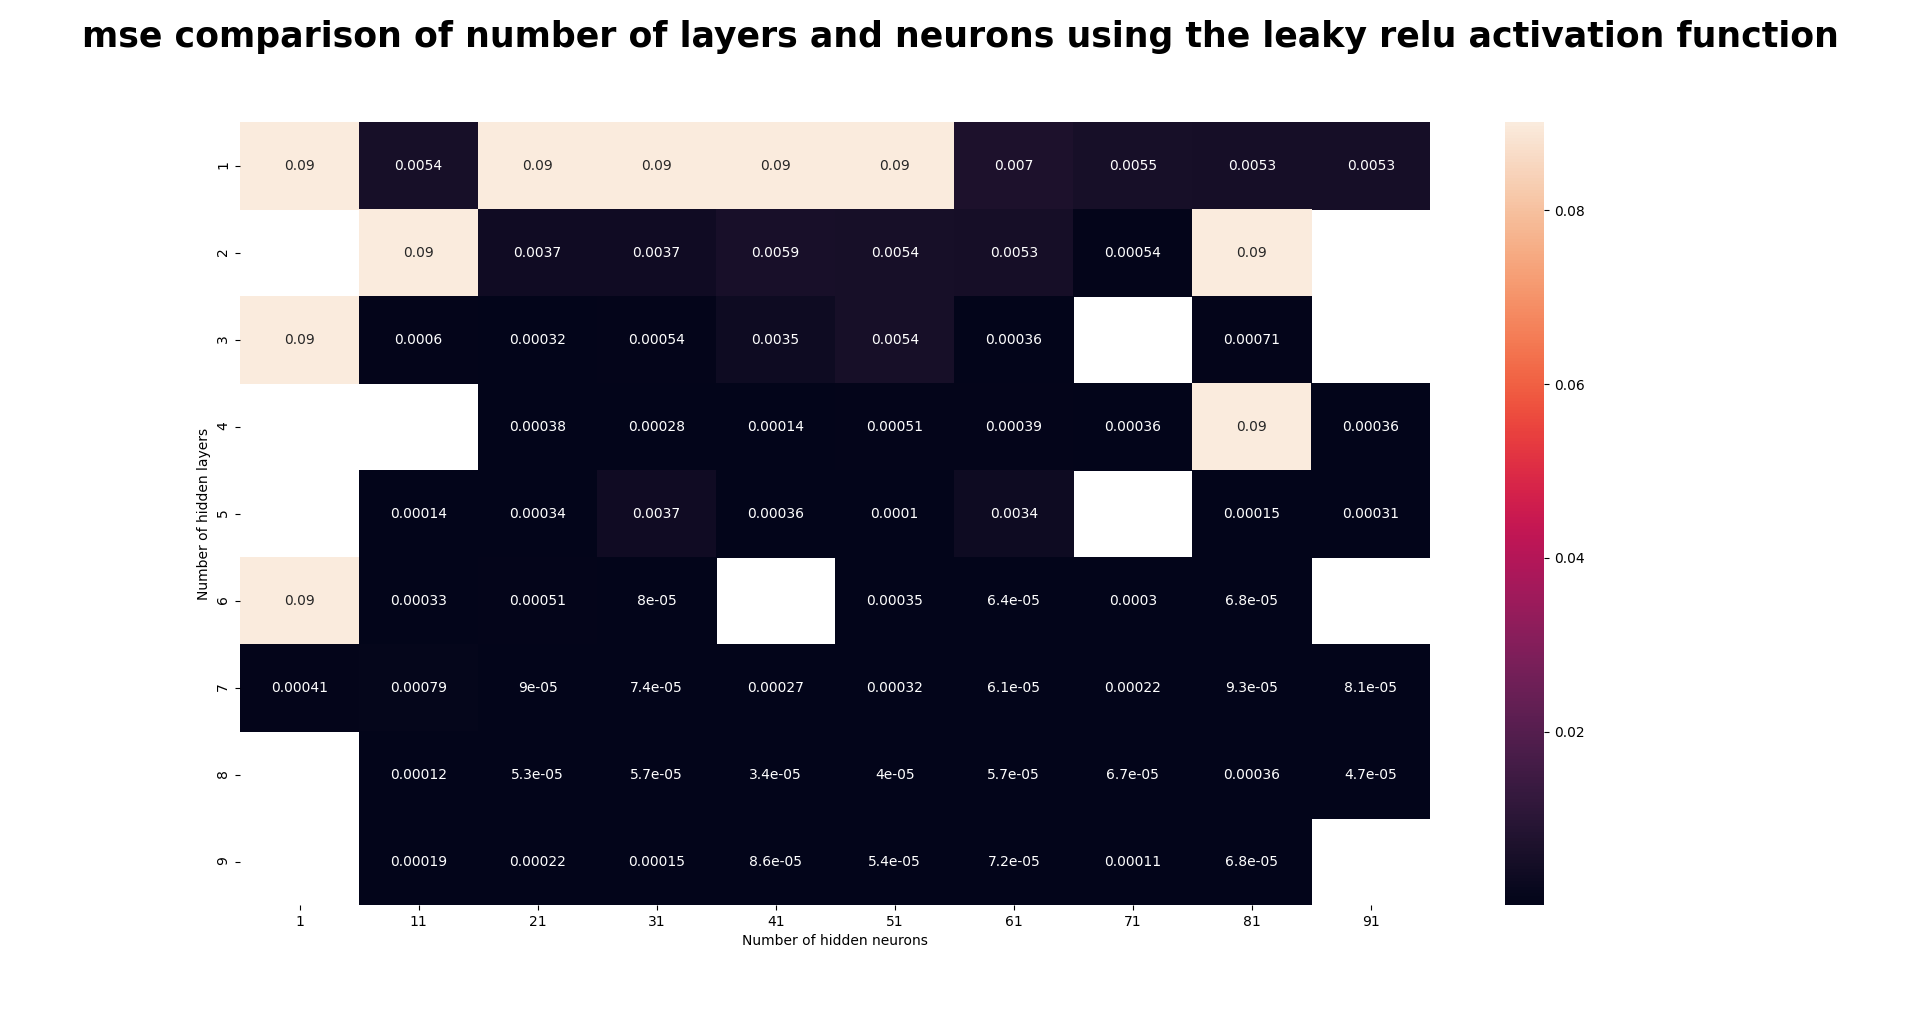
\includegraphics[width = 1\linewidth]{C:/Users/Sander/Documents/GitHub/FYS-STK4155/Project2/Project2/Report/Figures/heatmapRidge_TOTAL_leakyrelu_REAL.PNG}
\caption{\label{fig:heatmap8} Heatmap for different number of hidden layers and neurons using the leaky RELU activation function. This is the Ridge equivalent.}
\end{figure}

\noindent One can observe that my own implementation of RELU and leaky RELU is missing some values. This is due to overflow, and thus the MSE was put to NaN. However, if one compares the implementation in figures \ref{fig:heatmap6} and \ref{fig:heatmap8} to the OLS equivalent in figures \ref{fig:heatmap2} and \ref{fig:heatmap4}, one can observe that the overflow is less of a problem. This is due to the weight reduction applied by the Ridge $L_2$ norm which counteract some of the overflow. However, the overflow is still an issue for some hidden neuron/layer configurations. 
\\
The hidden neuron/layer configurations that does not experience overflow tend to perform very well. In fact, they are comparable to the Scikit RELU implementation in terms of MSE as can be seen when comparing figure \ref{fig:heatmap7} to figures \ref{fig:heatmap6} and \ref{fig:heatmap8}. However, the Scikit implementation seems much more stable, although it yields worse results for some hidden neuron/layer configurations.
\\
The sigmoid implementation seen in figure \ref{fig:heatmap5} does not experience overflow and is therefore more stable. From this figure one can observe that the MSE is relatively high for one hidden layer and one hidden neuron, but the MSE greatly decreases along with the hidden neurons and layers. This is due to the networks increased predictive capabilities created by the complexity of the network (more weights). We observe the same principle for the Scikit RELU implementation where there is no overflow and MSE decreases for increased number of hidden neurons and layers. However, as is the case for both the Scikit RELU and the sigmoid implementation, there seems to be a cap of how low the MSE will go. Additionally, this cap seems to be reached by most hidden neuron/layer configurations above one neuron and one layer, so picking any configuration in this area seems to be fine.

\newpage

\begin{center}
\Large{\textbf{Exercise d): Neural network classification}}
\end{center}

\begin{center}
\large{\textbf{Data set of hand-written digits}}
\end{center}

\noindent In this exercise we aim to classify hand-written digits given in the MNIST data set which can be downloaded from \href{{http://yann.lecun.com/exdb/mnist/}}{\nolinkurl{http://yann.lecun.com/exdb/mnist/}}. The data set contain both training data which will be used to train the neural network, and also test data which will be passed through the already trained network and compared to the actual answer. The data can be plotted and looks something like figure \ref{fig:DigitDataFig}

\begin{figure}[H]
\centering
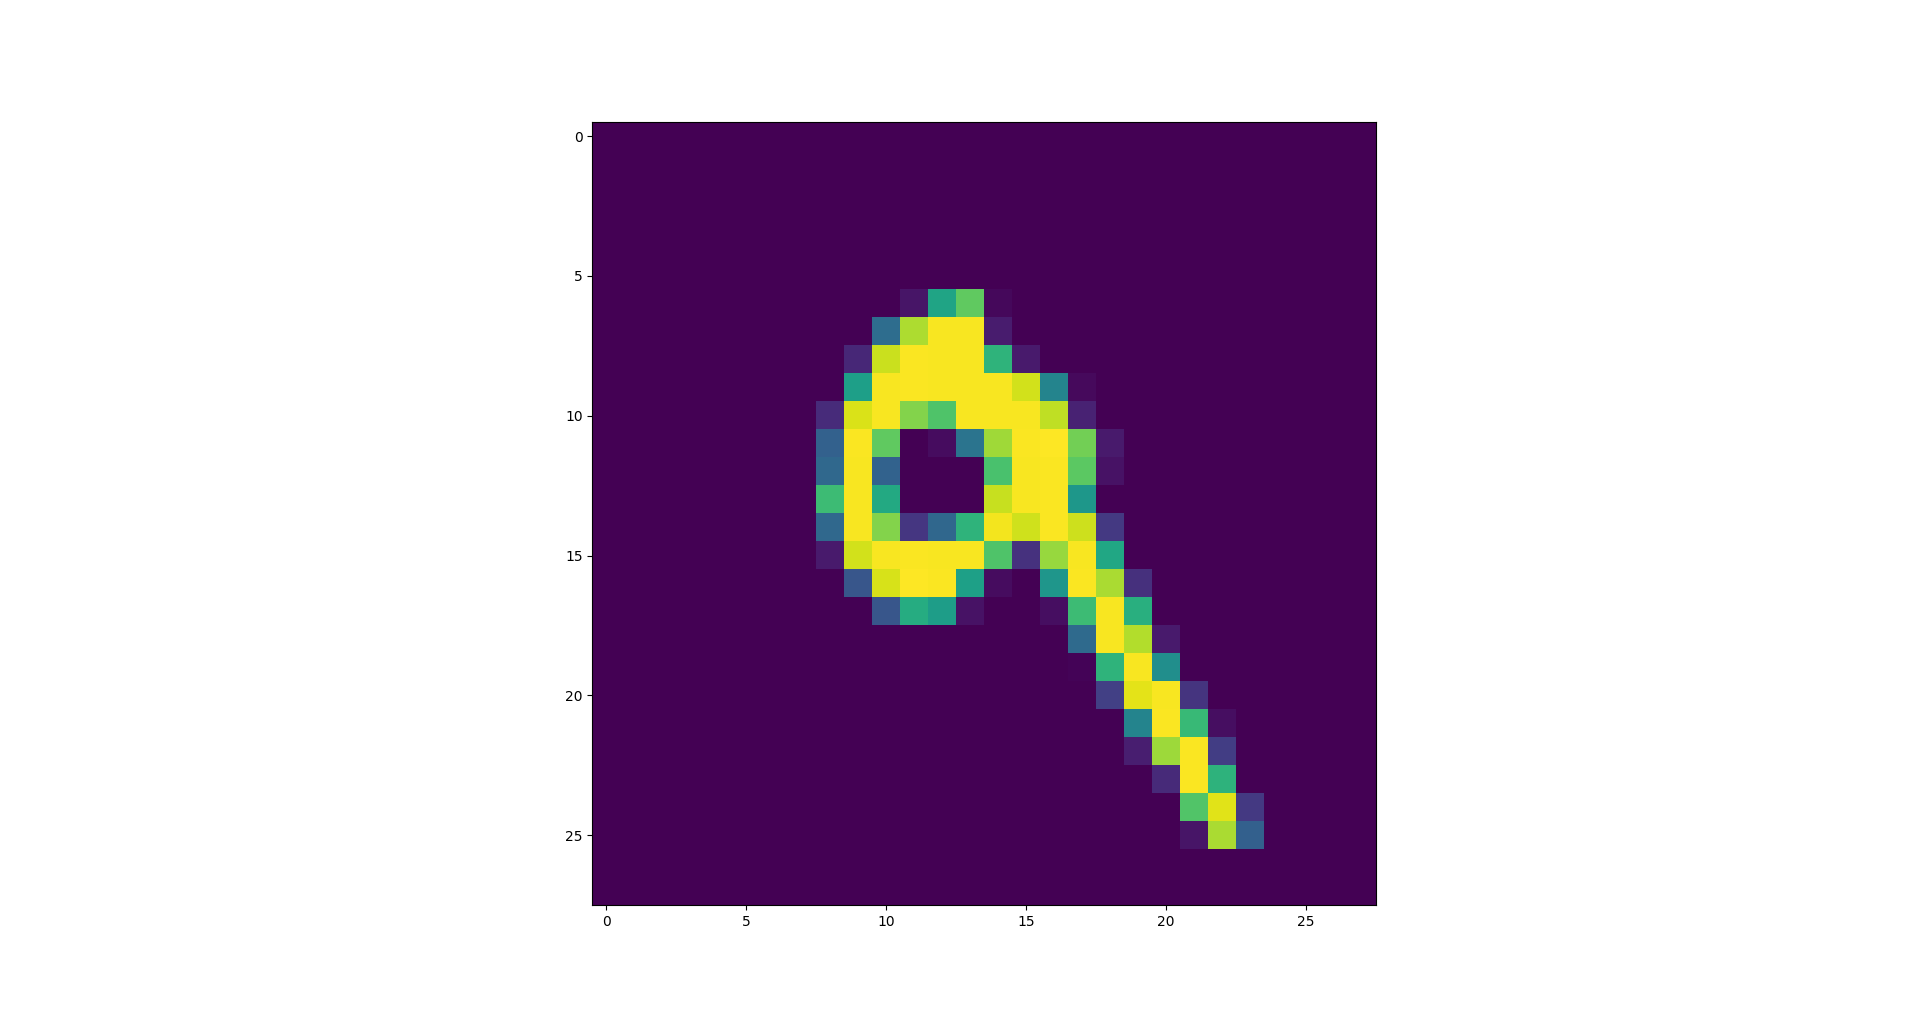
\includegraphics[width = 1\linewidth]{C:/Users/Sander/Documents/GitHub/FYS-STK4155/Project2/Project2/Report/Figures/DigitDataFig.PNG}
\caption{\label{fig:DigitDataFig} Example of how the training data looks. The digit shown is a hand-written digit that would be hard for a computer to recognize.}
\end{figure}

\noindent In this part of the exercise, we consider 1000 training images like figure \ref{fig:DigitDataFig} and 1000 testing images. This proved to be sufficient through testing for the neural network to perform well.

\begin{center}
\large{\textbf{Model evaluation principles}}
\end{center}

\noindent In order to evaluate a classification network we can no longer rely on the MSE or the $R^2$. Instead, we rely on using the accuracy score. The accuracy score is simply the correct number of prediction by the neural network divided by the total number of prediction (including wrong ones) and is defined by equation \ref{eq:acc}

\begin{equation}\label{eq:acc}
\begin{aligned}
\textrm{Accuracy} = \frac{\sum_{i = 1}^n I(f_i = y_i)}{n}
\end{aligned}
\end{equation}

\noindent where the numerator is the sum of correctly predicted digits and n is the total number of predictions. 

\begin{center}
\large{\textbf{The softmax activation function}}
\end{center}

\noindent The softmax function is a function that aims to take an input (what is passed through the neural network) and create a probability distribution of m different probabilities (m is 10 since we are working with the numbers from zero to nine). This function is given by equation \ref{eq:softmax}

\begin{equation}\label{eq:softmax}
\begin{aligned}
P(Y = y) = \frac{e^{\textbf{X}\beta}}{\sum_{i = 1}^m e^{\textbf{X}\beta}} 
\end{aligned}
\end{equation}

\noindent where \textbf{X} is the design matrix, $\beta$ is the regression coefficients matrix or weights in the neural network and P(Y = y) is the probability distribution of different possible outcomes from the neural network prediction. The softmax function allows us to categorize the input, digits in this case, into m different categories, 10 in this case, based on the probability estimated by the neural network. We can utilize the softmax function function as the output function in the output layer of the neural network, while the hidden layer activation functions can still be another function such as the sigmoid, RELU or leaky RELU. 

\begin{center}
\large{\textbf{Neural network classification results}}
\end{center}

\noindent We first take a look at how the neural network perform in terms of accuracy as function of different learning rates and hidden layer activation functions, as seen in figure \ref{fig:AccvsLrate}

\begin{figure}[H]
\centering
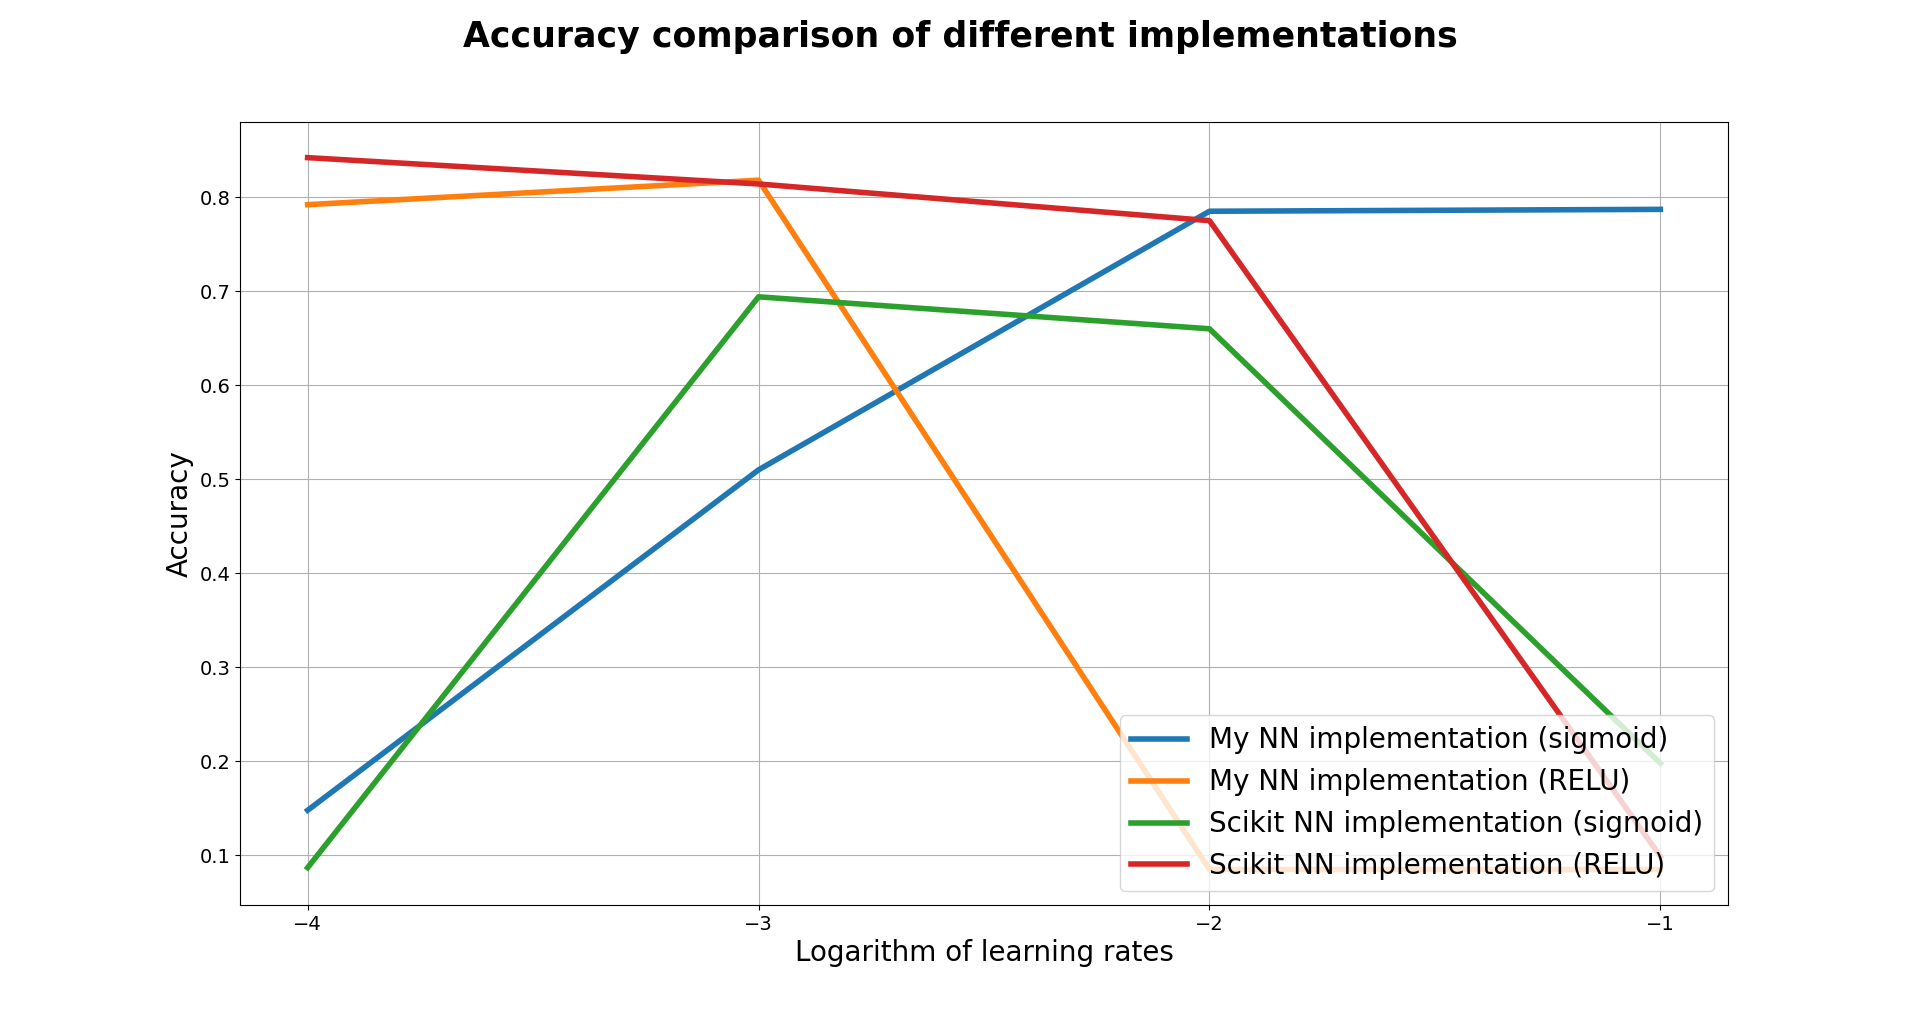
\includegraphics[width = 1\linewidth]{C:/Users/Sander/Documents/GitHub/FYS-STK4155/Project2/Project2/Report/Figures/final1.PNG}
\caption{\label{fig:AccvsLrate} Neural network accuracy in terms of learning rate and different activation functions.}
\end{figure}

\noindent It can be observed from figure \ref{fig:AccvsLrate} that my own implementation of the RELU activation function resembles that of the Scikit implementations at higher values of learning rates. However, my own RELU implementation experience severe overflow for lower values of the learning rate, leading to worse predictions. The Scikit an dmy own sigmoid implementation are very different. My implementation has its maximum accuracy at a learning rate of 0.1, while the Scikit implementation maxes out at 0.0001. Addtionally, my sigmoid implementation seems to only be improving with learning rate, while a common trend among the RELU and Scikit sigmoid implementation is that at the accuracy suddenly decrease at some given learning rate. It was observed that at this given learning rate yielded overflow in the neural network, meaning the neural network was unable to accurately predict the test set. This is despite taking measures against overflow such as the xavier initial weights and varied learning rate and step size. It is also observed from figure \ref{fig:AccvsLrate} that the RELU implementation seem to have a maximum accuracy over several different learning rates, or a cap, meaning picking a optimal learning rate from this cap yields good results.
\\
We now look towards finding the optimal number of neurons and layers in the neural network using the optimal learning rate found in figure \ref{fig:AccvsLrate}. This means a learning rate of 0.1 for my sigmoid implementation and a learning rate of 0.001 for my RELU implementation. We only consider hidden neurons between 1 and 100 and hidden layers between 1 and 10 as seen in figures \ref{fig:AccvsLrate2} and \ref{fig:AccvsLrate3}.

\begin{figure}[H]
\centering
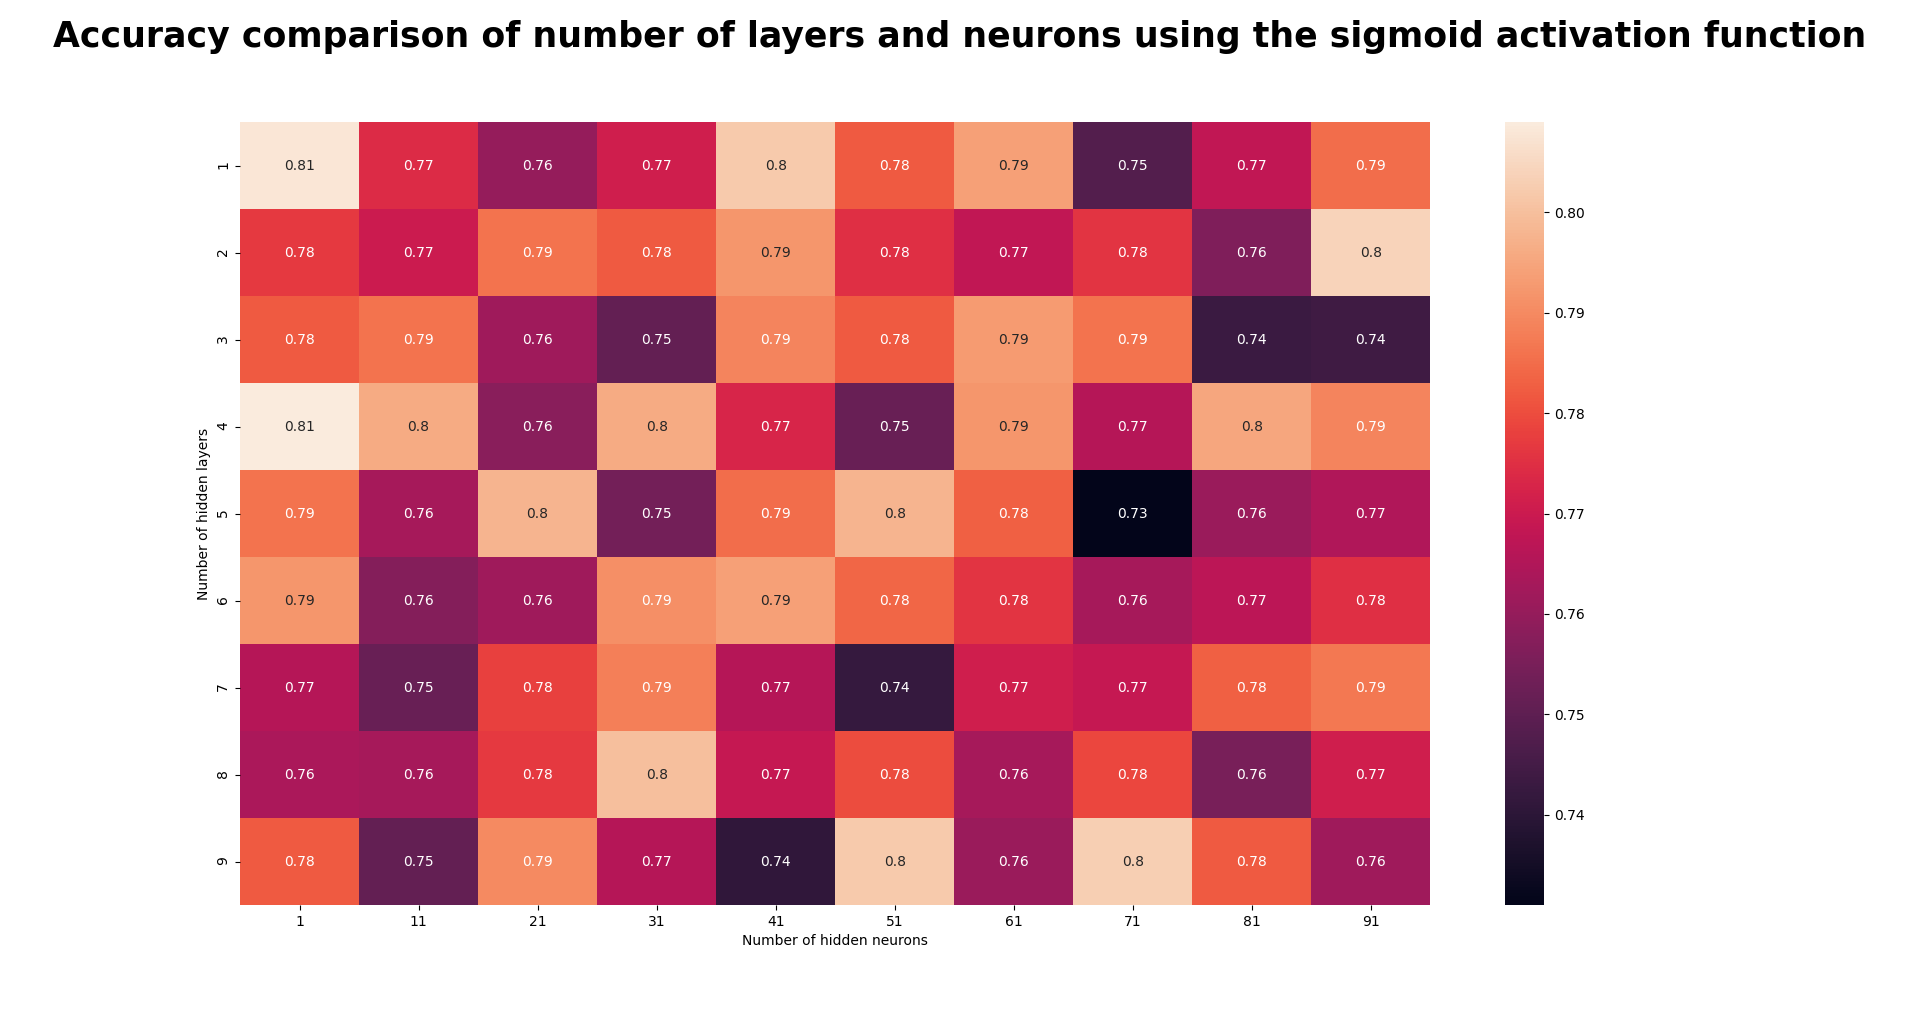
\includegraphics[width = 1\linewidth]{C:/Users/Sander/Documents/GitHub/FYS-STK4155/Project2/Project2/Report/Figures/final2.PNG}
\caption{\label{fig:AccvsLrate2} Accuracy for different configurations of hidden neurons and hidden layers.}
\end{figure}

\begin{figure}[H]
\centering
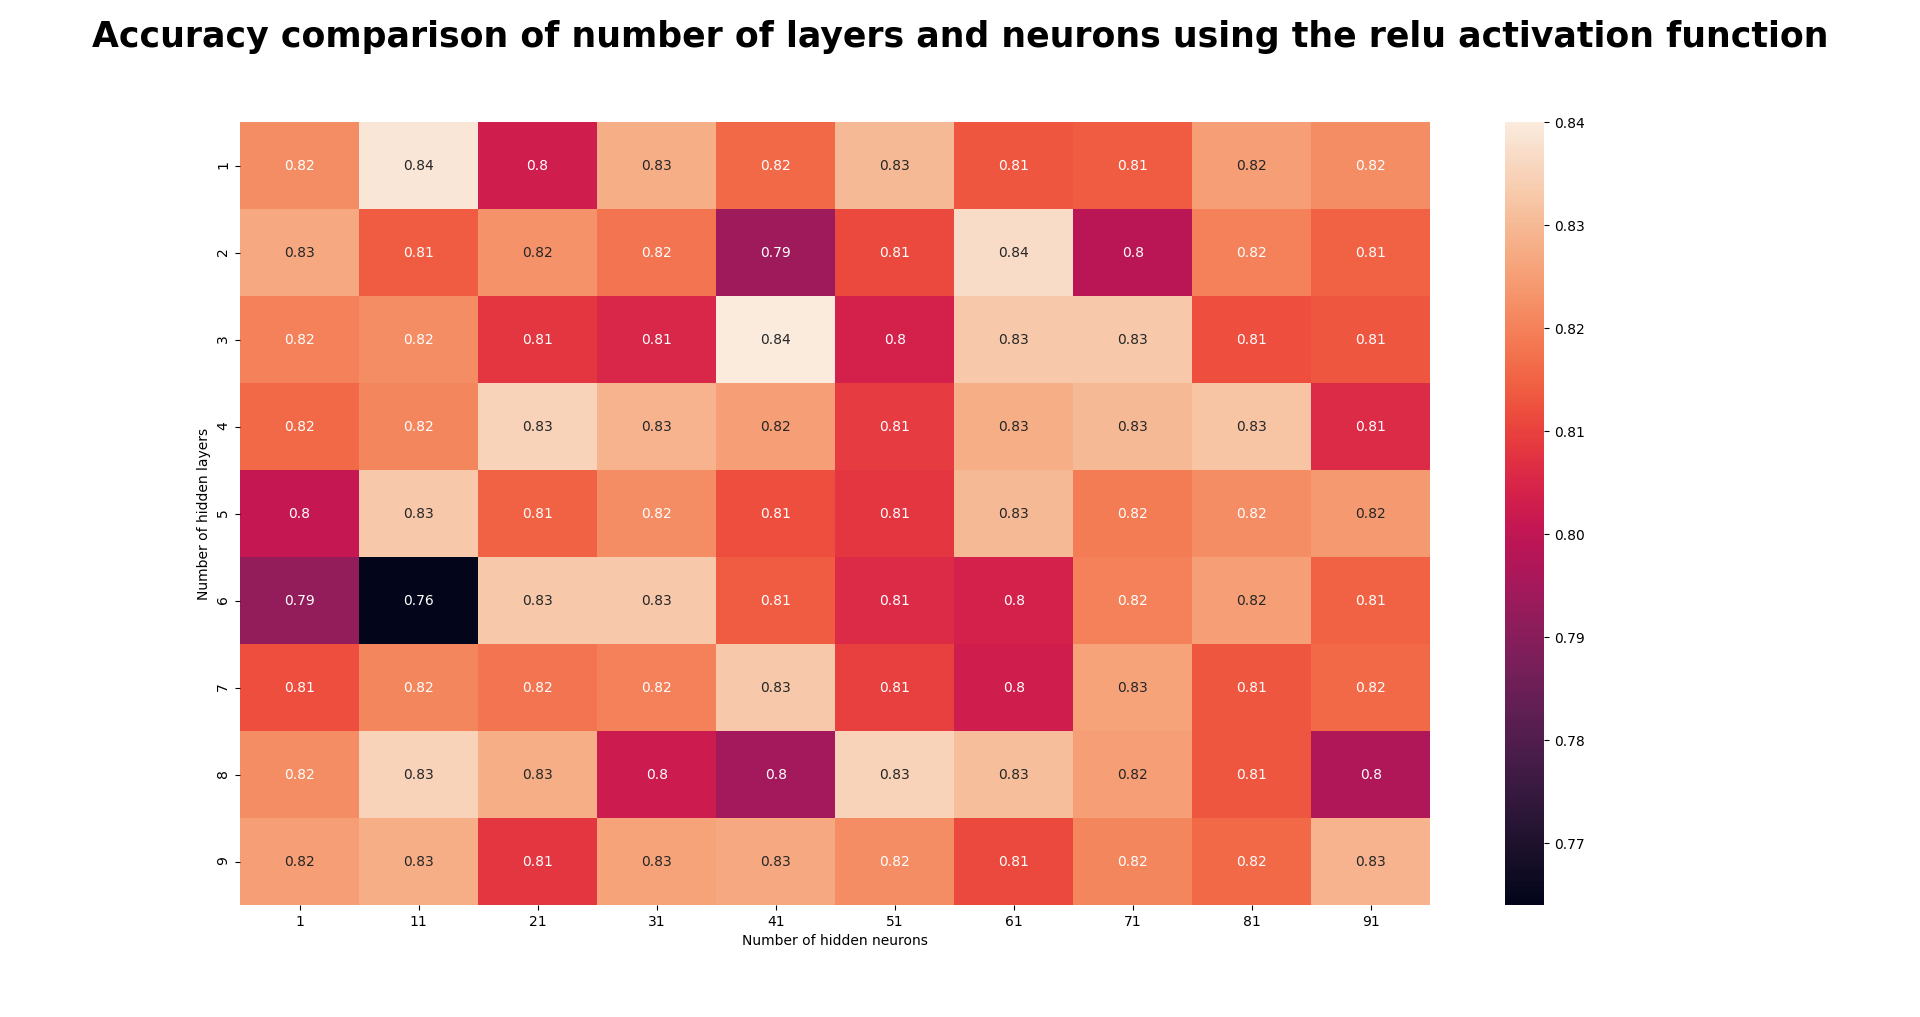
\includegraphics[width = 1\linewidth]{C:/Users/Sander/Documents/GitHub/FYS-STK4155/Project2/Project2/Report/Figures/final3.PNG}
\caption{\label{fig:AccvsLrate3} Accuracy for different configurations of hidden neurons and hidden layers.}
\end{figure}

\noindent It can be observed from figures \ref{fig:AccvsLrate2} and \ref{fig:AccvsLrate3} that the maximum accuracy for the sigmoid implementation is 0.8 and the maximum accuracy for the RELU implementation is 0.84. These values occur at several configurations of hidden neurons and layers, so picking any configuration with this accuracy should be fine. Having a accuracy rate of 0.8 means that $80\%$ of the digit images are successfully predicted. The baseline model has an accuracy of $0.1$ because if one were to randomly guess the test images one could expect to guess correctly $10\%$ of the time as we have 10 digits and 1 guess. Therefore, the neural network models is much better than the baseline model.
\\
We now aim to apply the $L_2$ norm, that is, perform the Ridge regression equivalent. We again aim to find the optimal learning rate, but also the optimal penalty parameter $\lambda$. Figures \ref{fig:AccvsLrate4} and \ref{fig:AccvsLrate5} shows a heatmap of different learning rates and penalty values.

\begin{figure}[H]
\centering
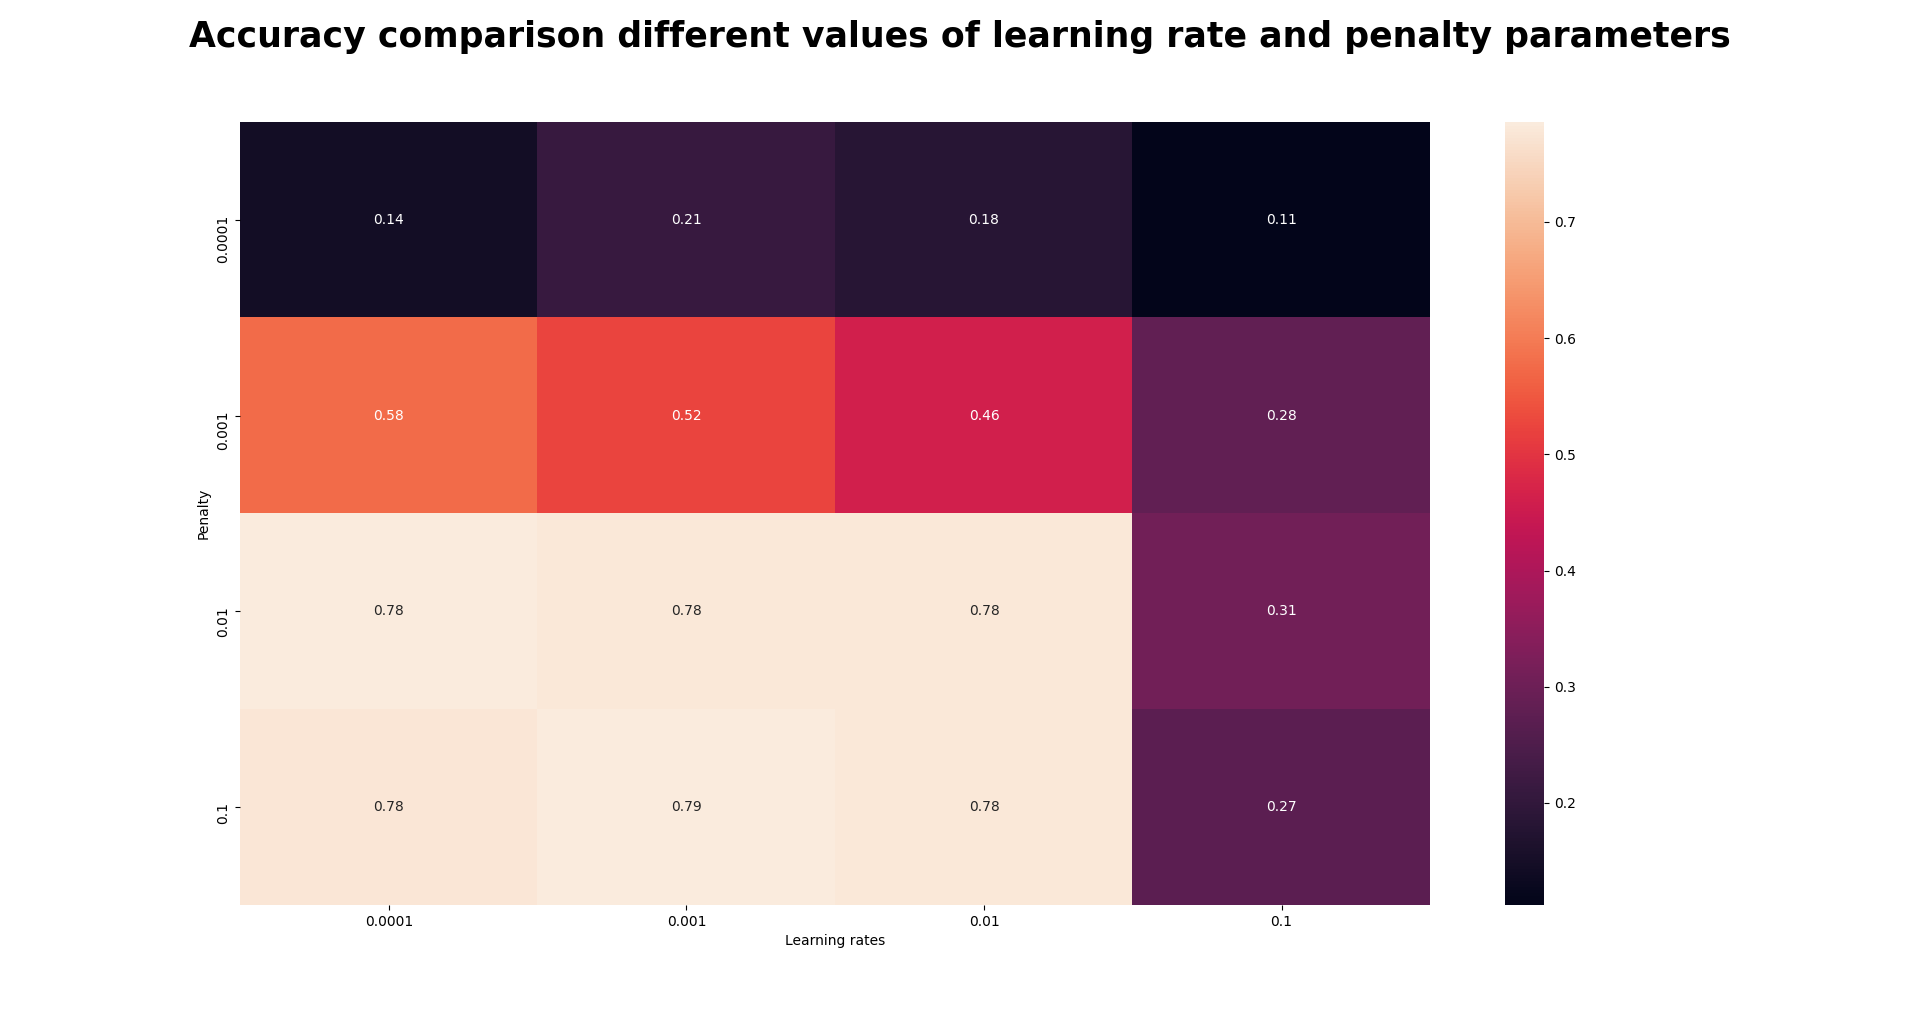
\includegraphics[width = 1\linewidth]{C:/Users/Sander/Documents/GitHub/FYS-STK4155/Project2/Project2/Report/Figures/final10.PNG}
\caption{\label{fig:AccvsLrate4} Accuracy for Ridge regression equivalent neural network for different learning rates and penalties using the sigmoid activation function.}
\end{figure}

\begin{figure}[H]
\centering
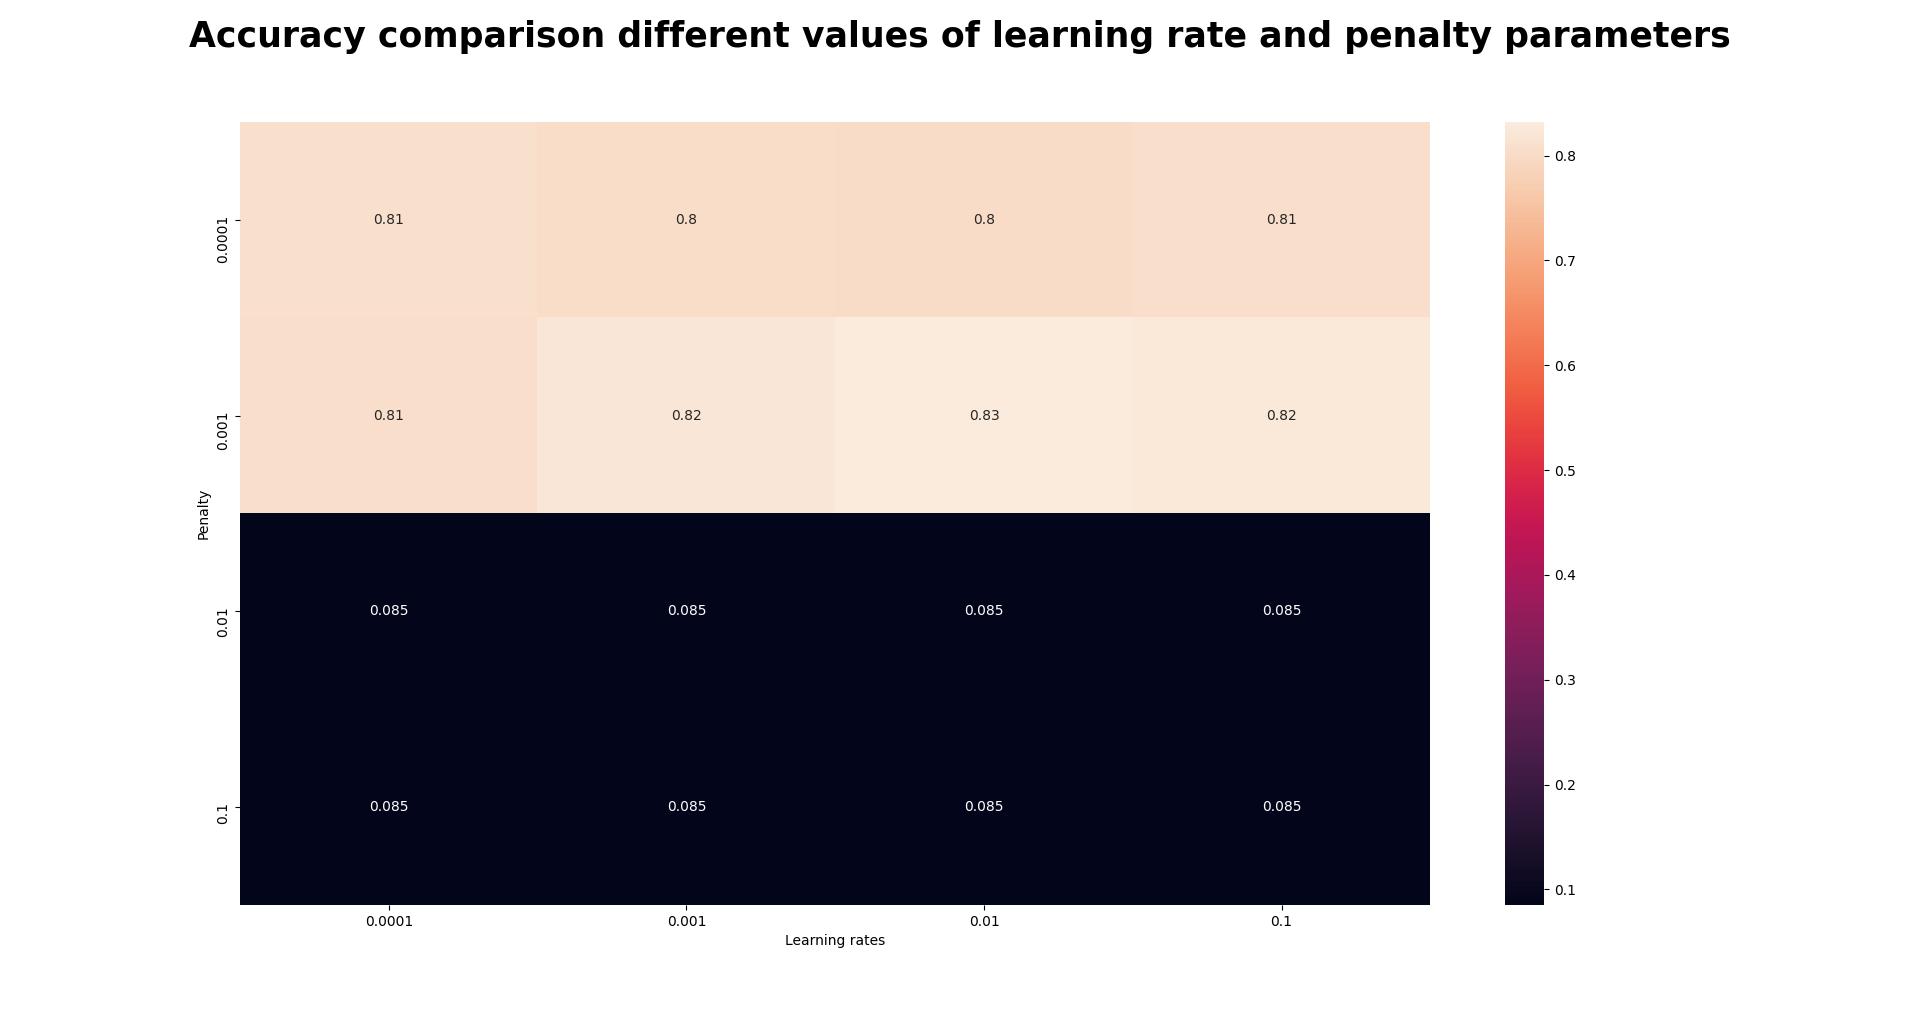
\includegraphics[width = 1\linewidth]{C:/Users/Sander/Documents/GitHub/FYS-STK4155/Project2/Project2/Report/Figures/final11.PNG}
\caption{\label{fig:AccvsLrate5} Accuracy for Ridge regression equivalent neural network for different learning rates and penalties using the RELU activation function.}
\end{figure}

\noindent It can be observed that the sigmoid implementation in figure \ref{fig:AccvsLrate4} that the network prefers higher penalty and lower learning rates while the RELU implementation in figure \ref{fig:AccvsLrate5} seems to prefer lower penalty. It is also observed that the sigmoid implementation is sensitive to both the penalty while the RELU implementation is mostly sensitive to the penalty. It seems to be a threshold where the accuracy drops significantly as a given penalty. The sigmoid implementation on the other hand is more delicate where there is no threshold, but rather a smooth increase in accuracy towards lower learning rate and higher penalty.
\\
We can now see how the Ridge equivalent neural network behaves as function of the number of hidden neurons and hidden layers as seen in figures \ref{fig:AccvsLrate6} and \ref{fig:AccvsLrate7}.

\begin{figure}[H]
\centering
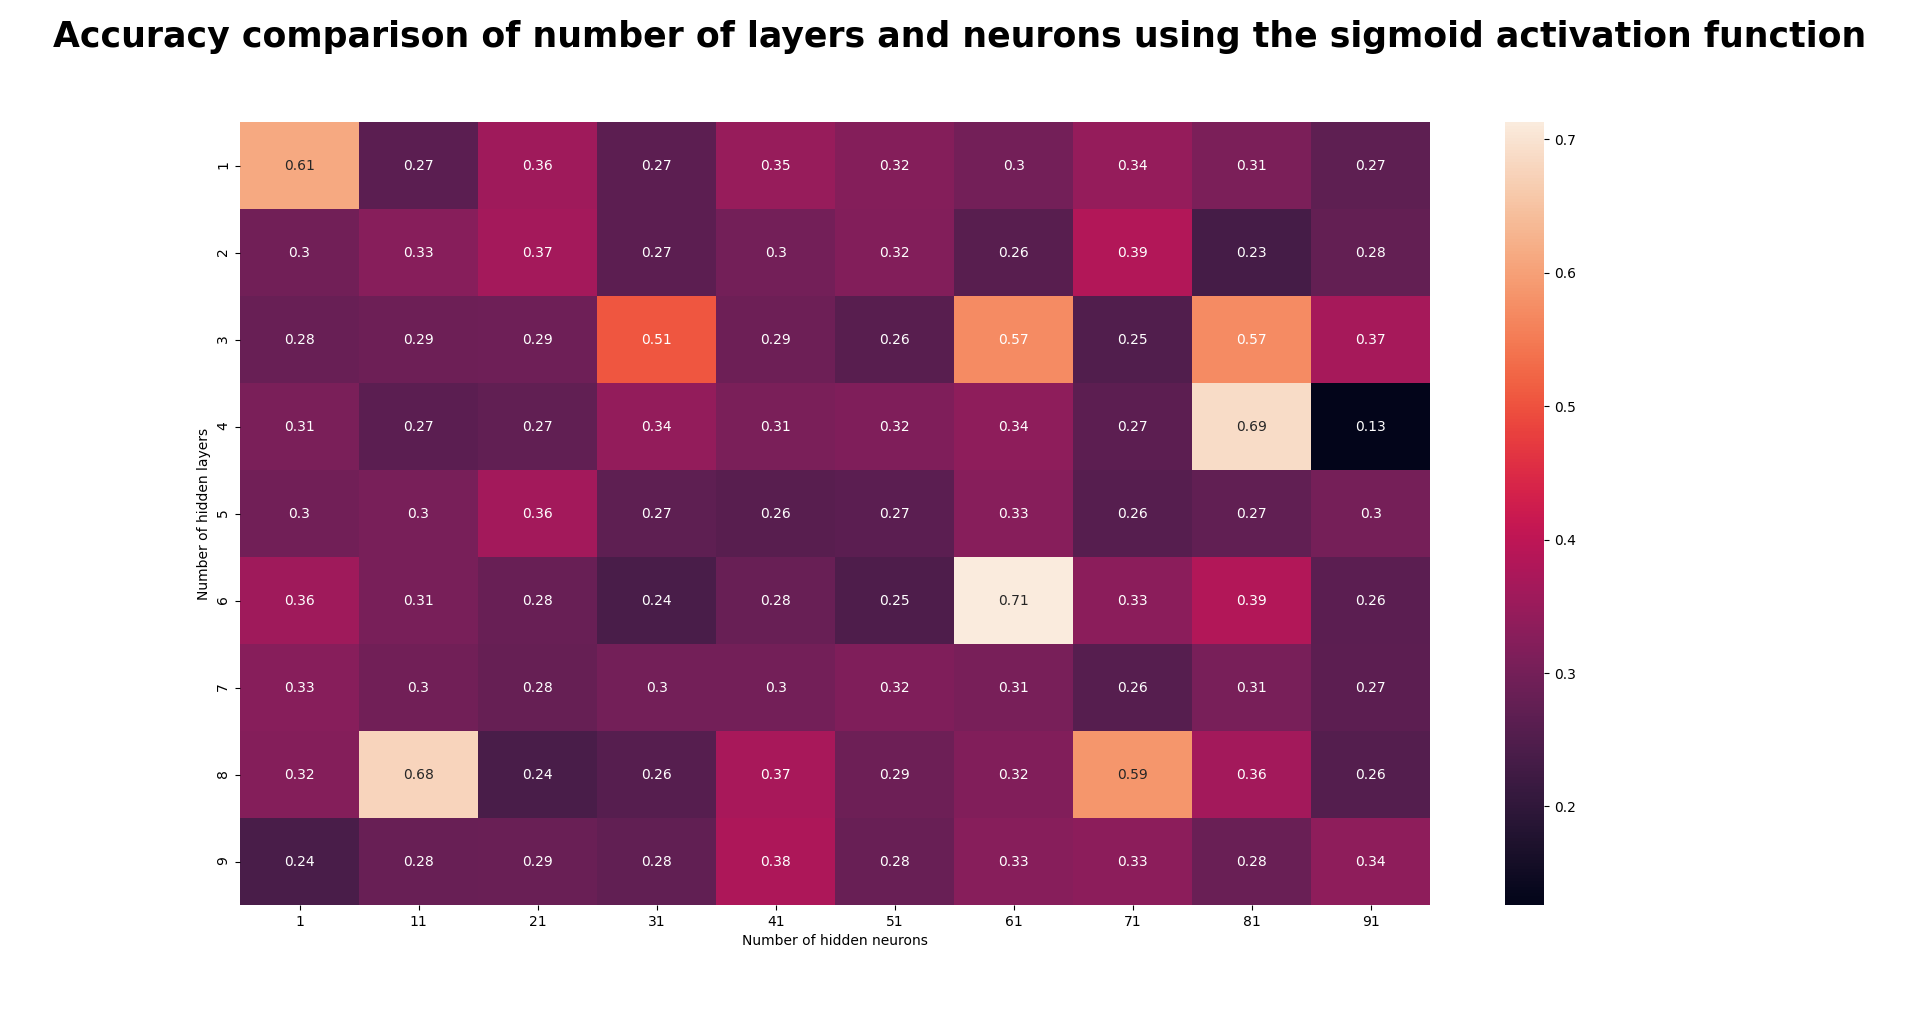
\includegraphics[width = 1\linewidth]{C:/Users/Sander/Documents/GitHub/FYS-STK4155/Project2/Project2/Report/Figures/final6.PNG}
\caption{\label{fig:AccvsLrate6} Accuracy for Ridge regression equivalent neural network for different hidden neuron/layer configurations using the sigmoid activation function.}
\end{figure}

\begin{figure}[H]
\centering
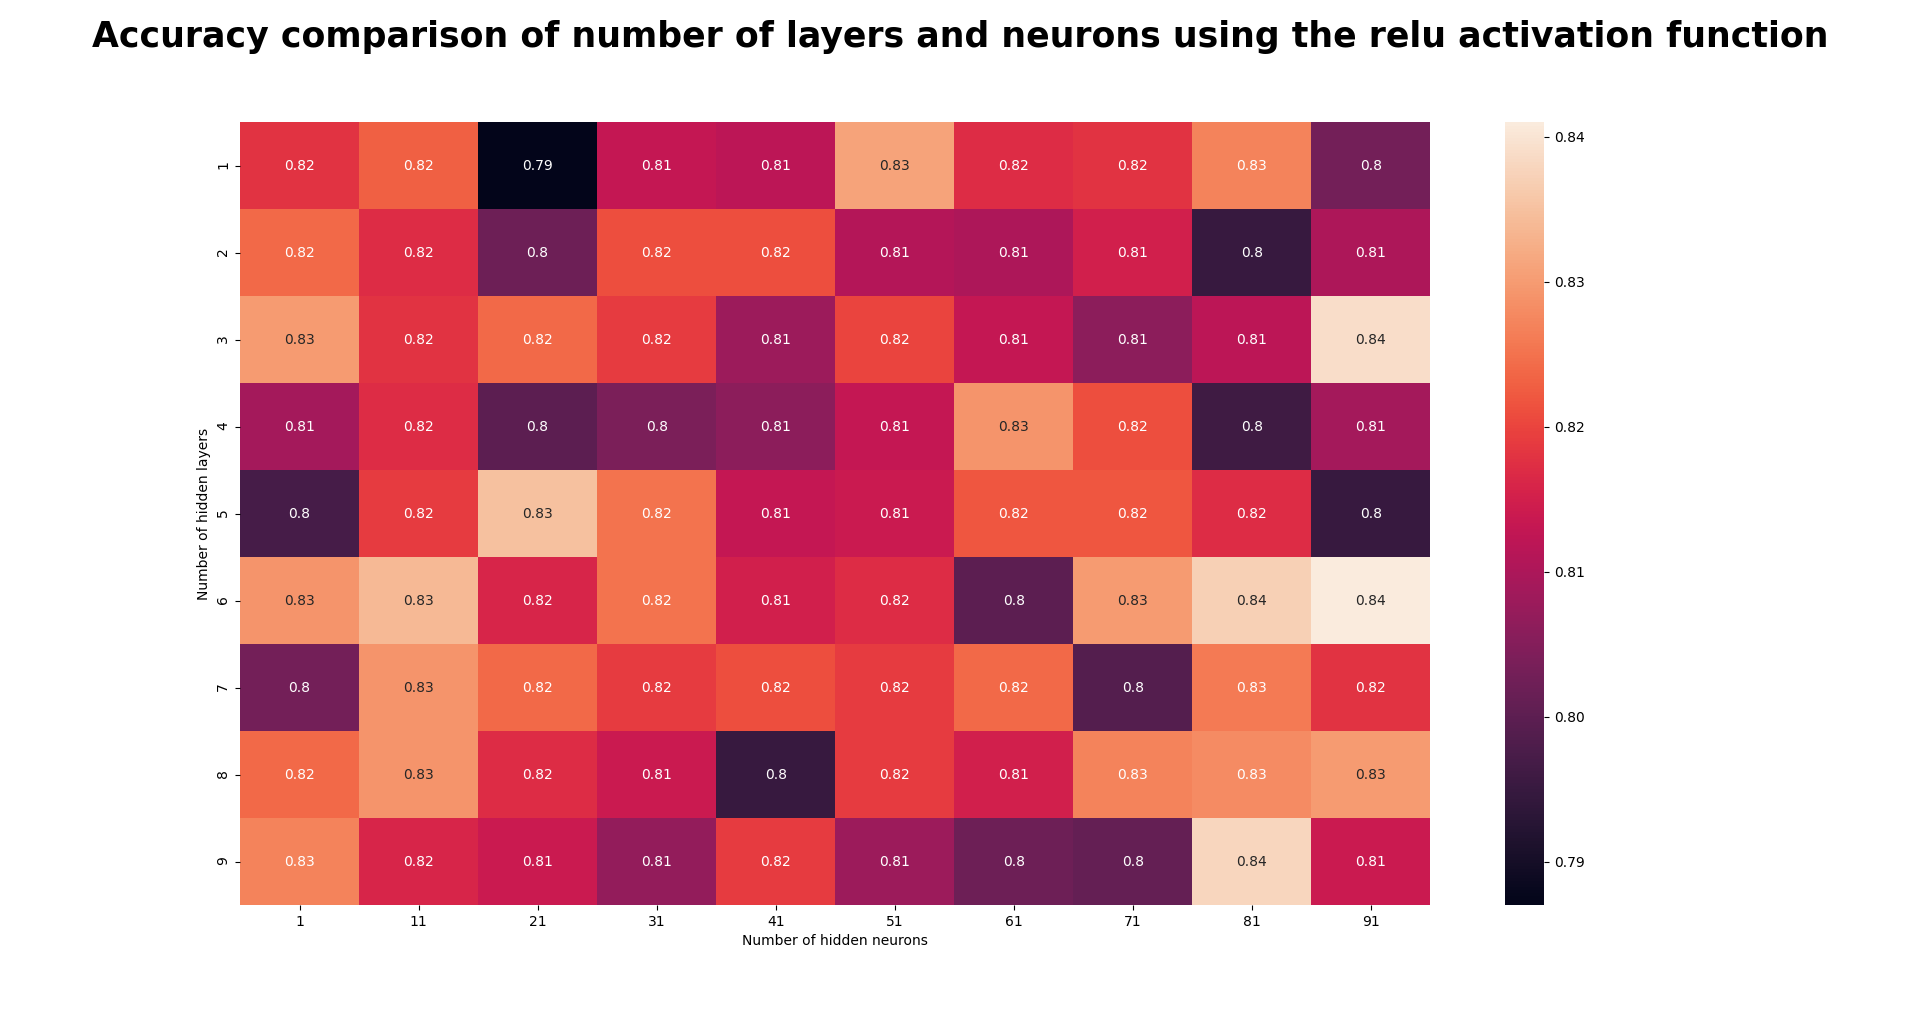
\includegraphics[width = 1\linewidth]{C:/Users/Sander/Documents/GitHub/FYS-STK4155/Project2/Project2/Report/Figures/final7.PNG}
\caption{\label{fig:AccvsLrate7} Accuracy for Ridge regression equivalent neural network for different hidden neuron/layer configurations using the RELU activation function.}
\end{figure}

\noindent It can be observed when comparing figures \ref{fig:AccvsLrate6} and \ref{fig:AccvsLrate7} that the sigmoid implementation performs worse than the RELU implementation, as the optimal model for the sigmoid implementation yields an accuracy of $0.71$ at most while the RELU implementation yields an accuracy of $0.84$ at most. This means that the RELU function itself increases the chance for the neural network to predict the hand-written digit by $13\%$ relative to a model using the sigmoid function. It is also observed that the sigmoid implementation in figure \ref{fig:AccvsLrate6} is very sensitive to the configuration of the network as the accuracy drops significantly for most configurations of hidden neurons/layers. This is not the case with the RELU implementation as seen in figure \ref{fig:AccvsLrate7} where the accuracy is above $0.8$ for nearly every hidden neuron/layer configuration. 

\newpage

\begin{center}
\Large{\textbf{Exercise e): Logistic SGD}}
\end{center}

\noindent In this exercise, we aim to utilize the SGD algorithm developed in exercise 1a), but for logistic regression on the MNIST digit data. The algorithm will be the same as described in exercise 1a), but where the softmax is utilized in the gradient of the loss function to give a probability distribution for the different digits. The algorithm is implemented for both the OLS and Ridge equivalent SGDs for both my own SGD algorithm and the Scikit SGD algorithm. The accuracy resulting said algorithms with different penalties are plotted versus the learning rate in figure \ref{fig:finalAcc1}.

\begin{figure}[H]
\centering
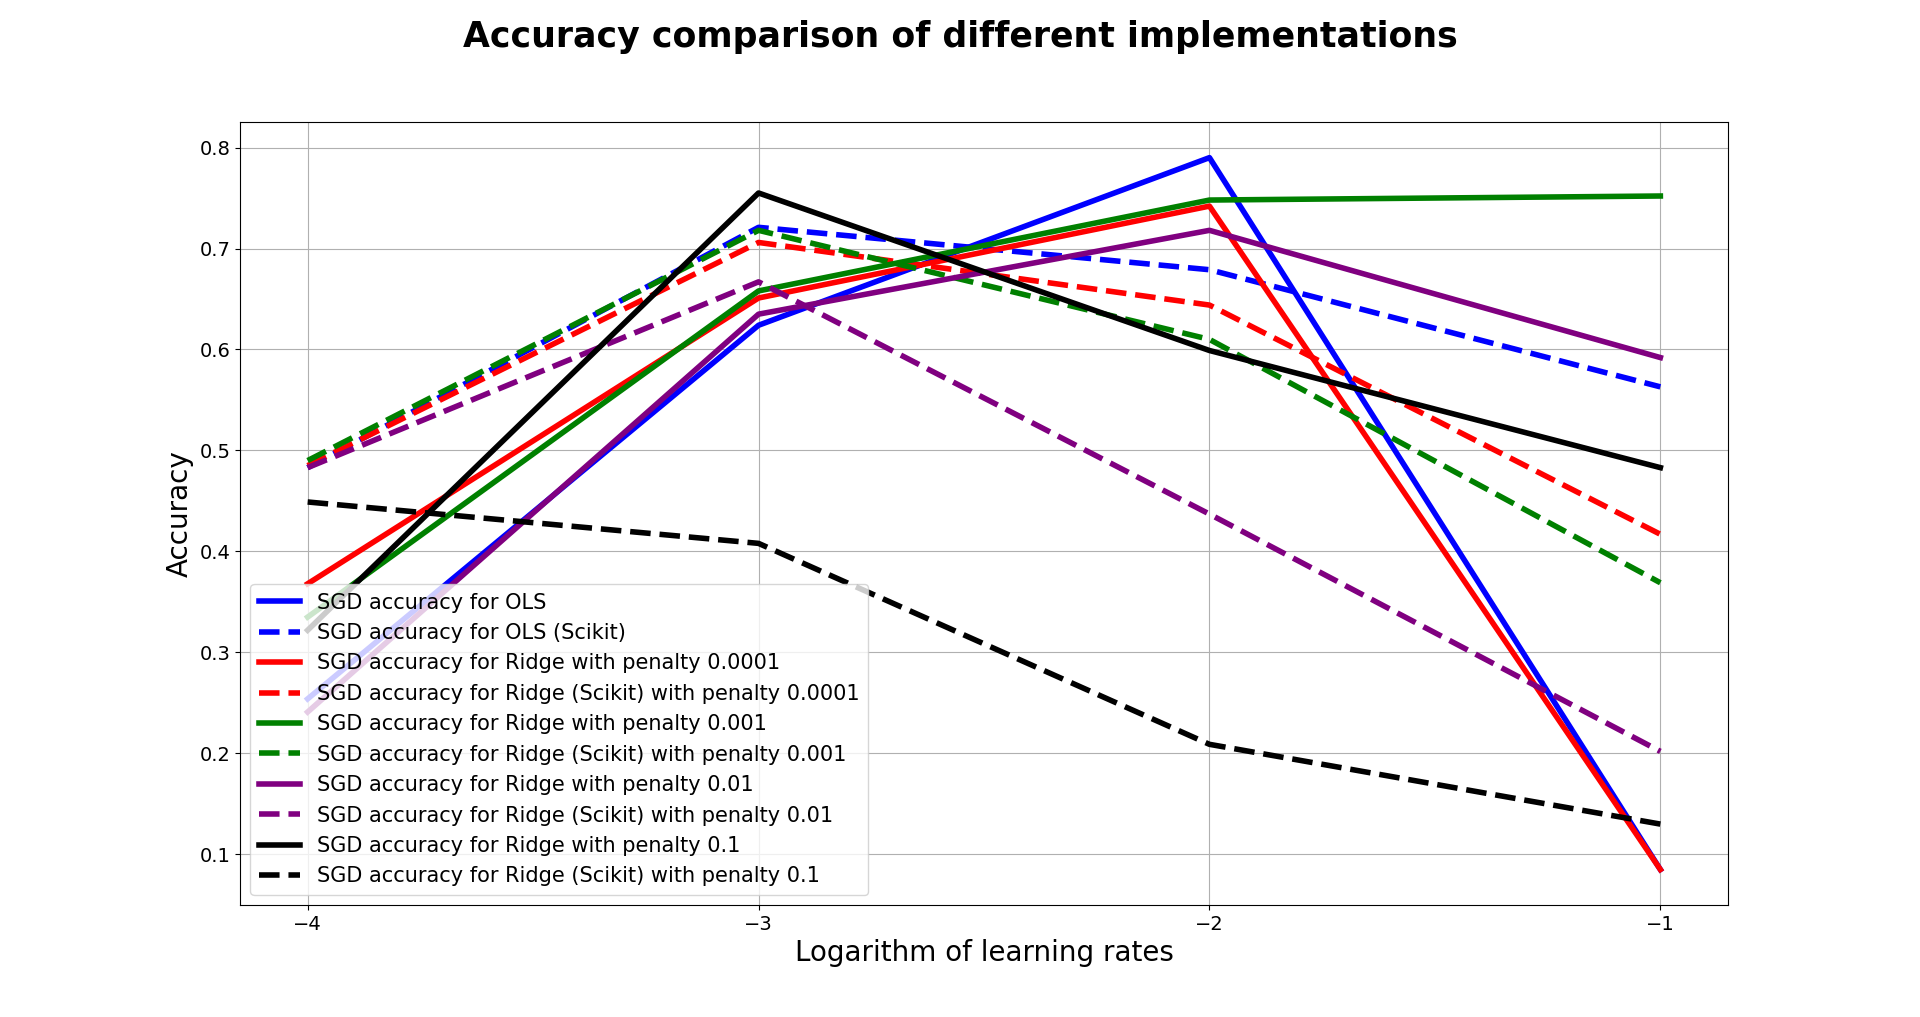
\includegraphics[width = 1\linewidth]{C:/Users/Sander/Documents/GitHub/FYS-STK4155/Project2/Project2/Report/Figures/finalAcc1.PNG}
\caption{\label{fig:finalAcc1} Accuracy for logistic SGD for both OLS and Ridge equivalent implementations using both the Scikit and my own SGD algorithm. The results from the Scikit implementation is dashed and same color lines represent models with same $L_2$ penalty.}
\end{figure}

\noindent One can observe from figure \ref{fig:finalAcc1} that my own implementation is comparable with the Scikit implementation. The accuracy values are about the same, but their maximum occurs at different learning rates. However, the plot is a little messy so the plot is divided into two different plots, the first one being the results from my own SGD implementation and the second one being the Scikit implementation.

\begin{figure}[H]
\centering
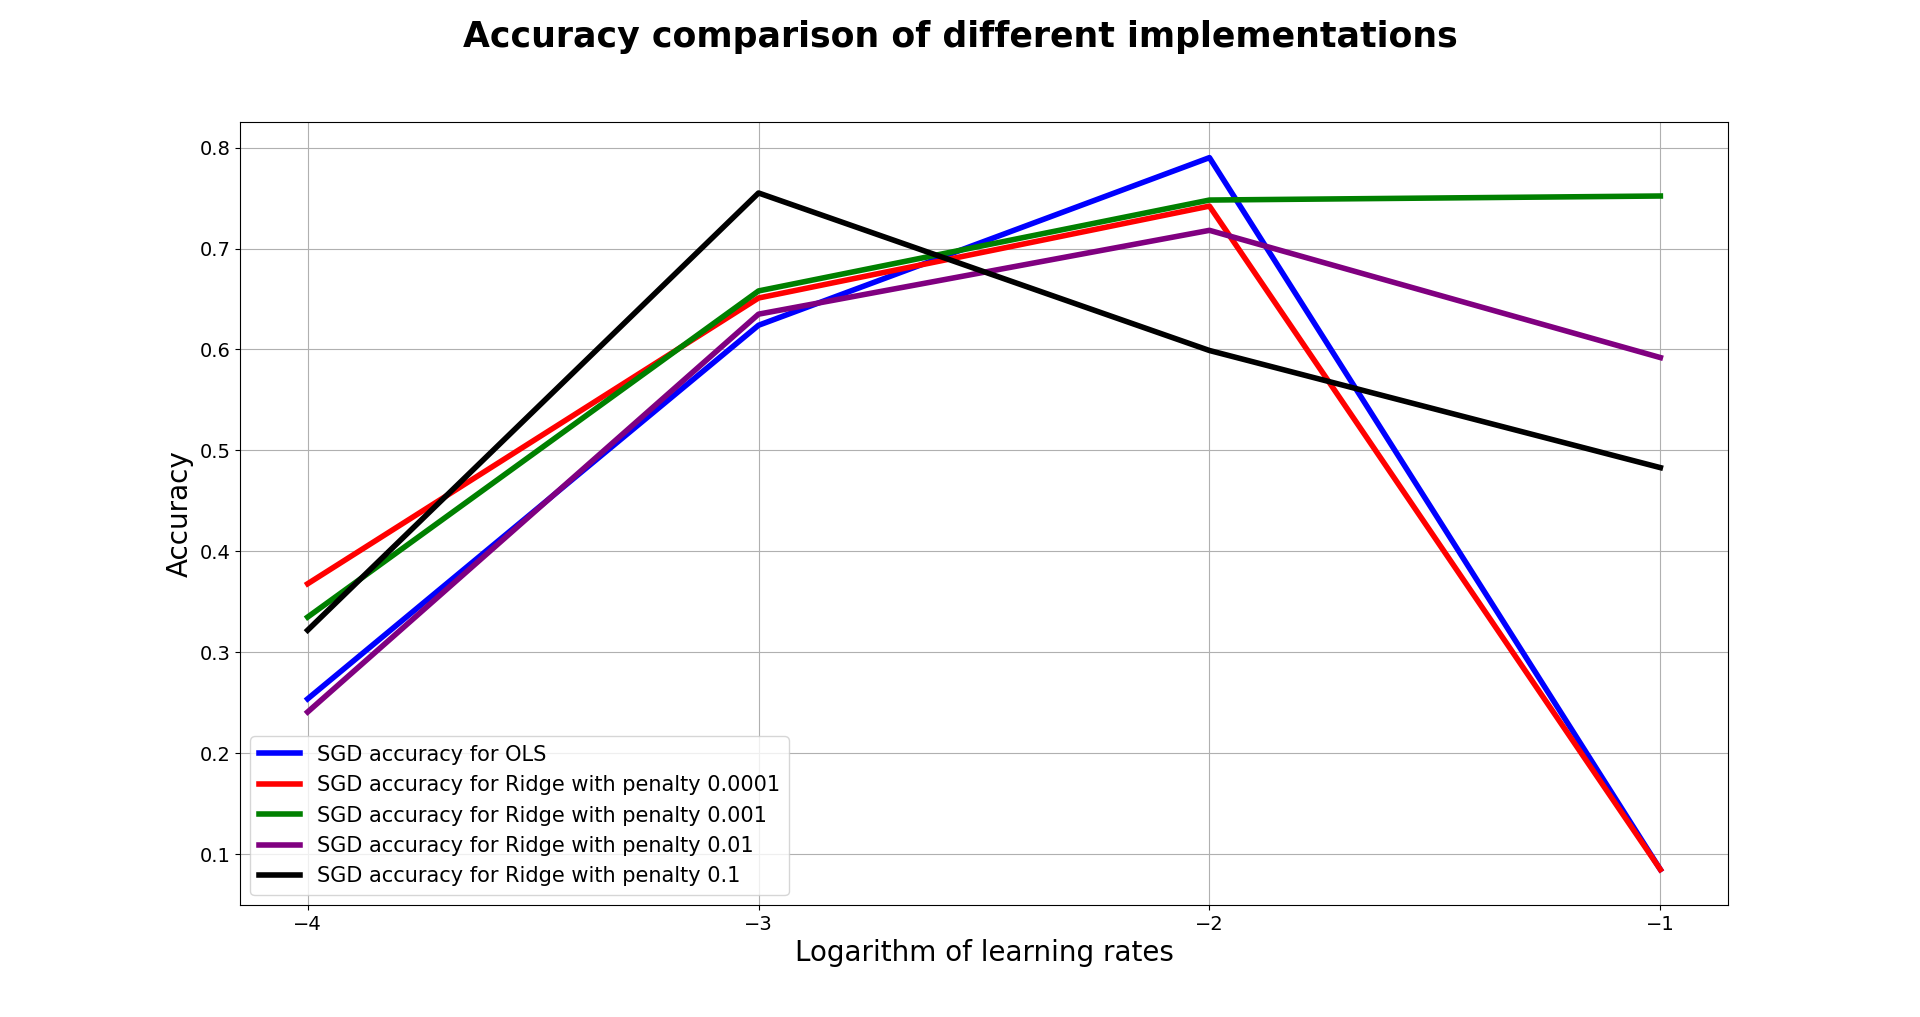
\includegraphics[width = 1\linewidth]{C:/Users/Sander/Documents/GitHub/FYS-STK4155/Project2/Project2/Report/Figures/finalAcc2.PNG}
\caption{\label{fig:finalAcc2} Accuracy for logistic SGD for both OLS and Ridge equivalent implementations using my own SGD algorithm.}
\end{figure}

\begin{figure}[H]
\centering
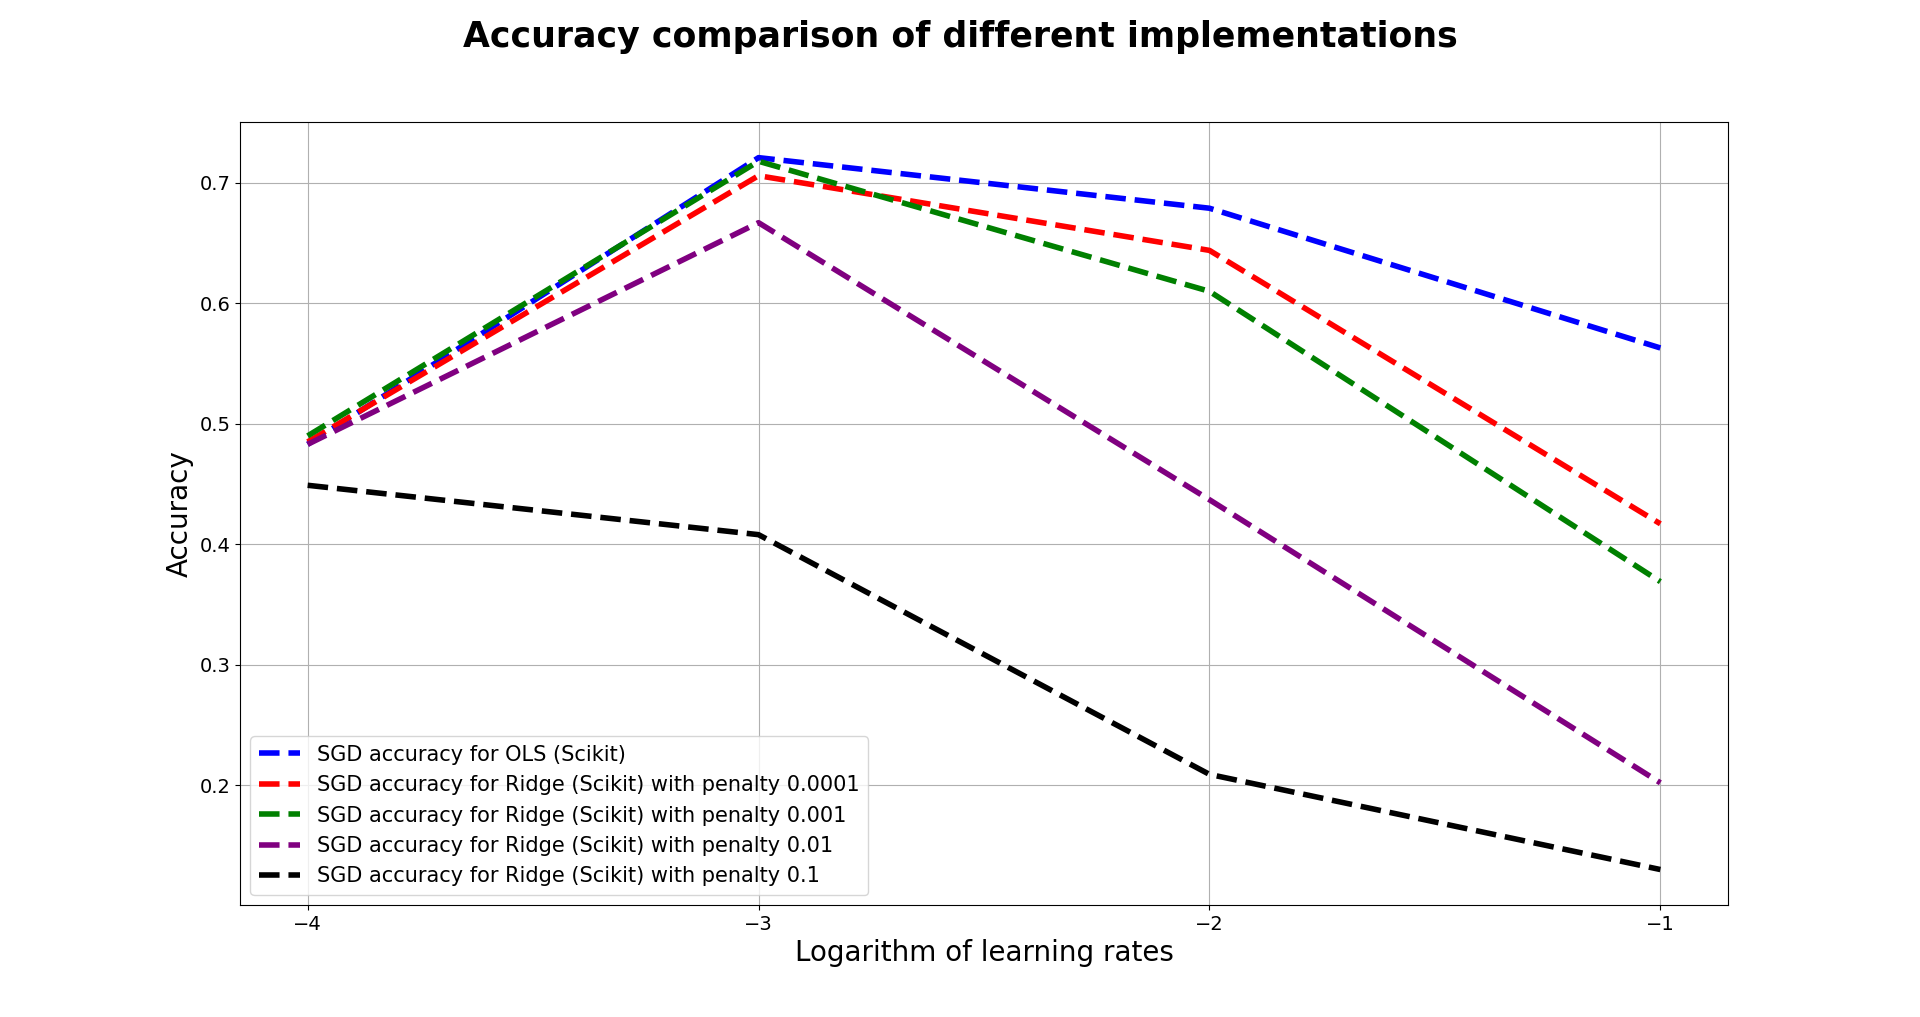
\includegraphics[width = 1\linewidth]{C:/Users/Sander/Documents/GitHub/FYS-STK4155/Project2/Project2/Report/Figures/finalAcc3.PNG}
\caption{\label{fig:finalAcc3} Accuracy for logistic SGD for both OLS and Ridge equivalent implementations using the Scikit SGD algorithm.}
\end{figure}

\noindent One can observe from figures \ref{fig:finalAcc2} and \ref{fig:finalAcc3} that my own algorithms achieves higher accuracy than the Scikit implementation when comparing similar penalties. As for my own implementation, one observes that the OLS and most Ridge equivalent models have the same optimal learning rate at $0.01$ (except for $\lambda = 0.1, 0.001$). Ridge models with a low penalty tens to lie close to the OLS for any learning rate (since a penalty of zero is equivalent to the OLS), but one can observe that penalties higher or equal to $0.001$ deviates from the OLS model. The model with penalty $0.1$ actually performs better than the OLS for learning rates equal to $0.0001$, $0.001$ and $0.1$, but performs worse for a learning rate of $0.01$. Ridge models with a high penalty tends to outperform the OLS everywhere but the learning rate of $0.01$. In fact the models using a penalty of $0.001$ keep increasing after the other models peak at a learning rate of $0.01$. A similar behaviour can be observe from the model using a penalty of $0.01$ as well, but the accuracy actually decreases after the other models peak.
\\
One also observe from the Scikit implementation that the models using different penalties are pretty similar for learning rates lower than $0.001$ (except for the model using a penalty of $0.1$). However, for learning rates higher than $0.001$, the models starts to deviate from one another. One can observe that increasing the penalty yields lower overall accuracy. In fact. it is the OLS equivalent model (blue lines) that achieve the highest overall accuracy. The difference in the models continue to increase when the learning rate increases. Another important observations is that the optimal learning rate of all the Scikit implementations are equal except for the model using a penalty of $0.1$.
\\
We now aim to find the optimal penalty and learning rate for the Ridge models as seen in figures \ref{fig:finalAcc4} and \ref{fig:finalAcc5}.

\begin{figure}[H]
\centering
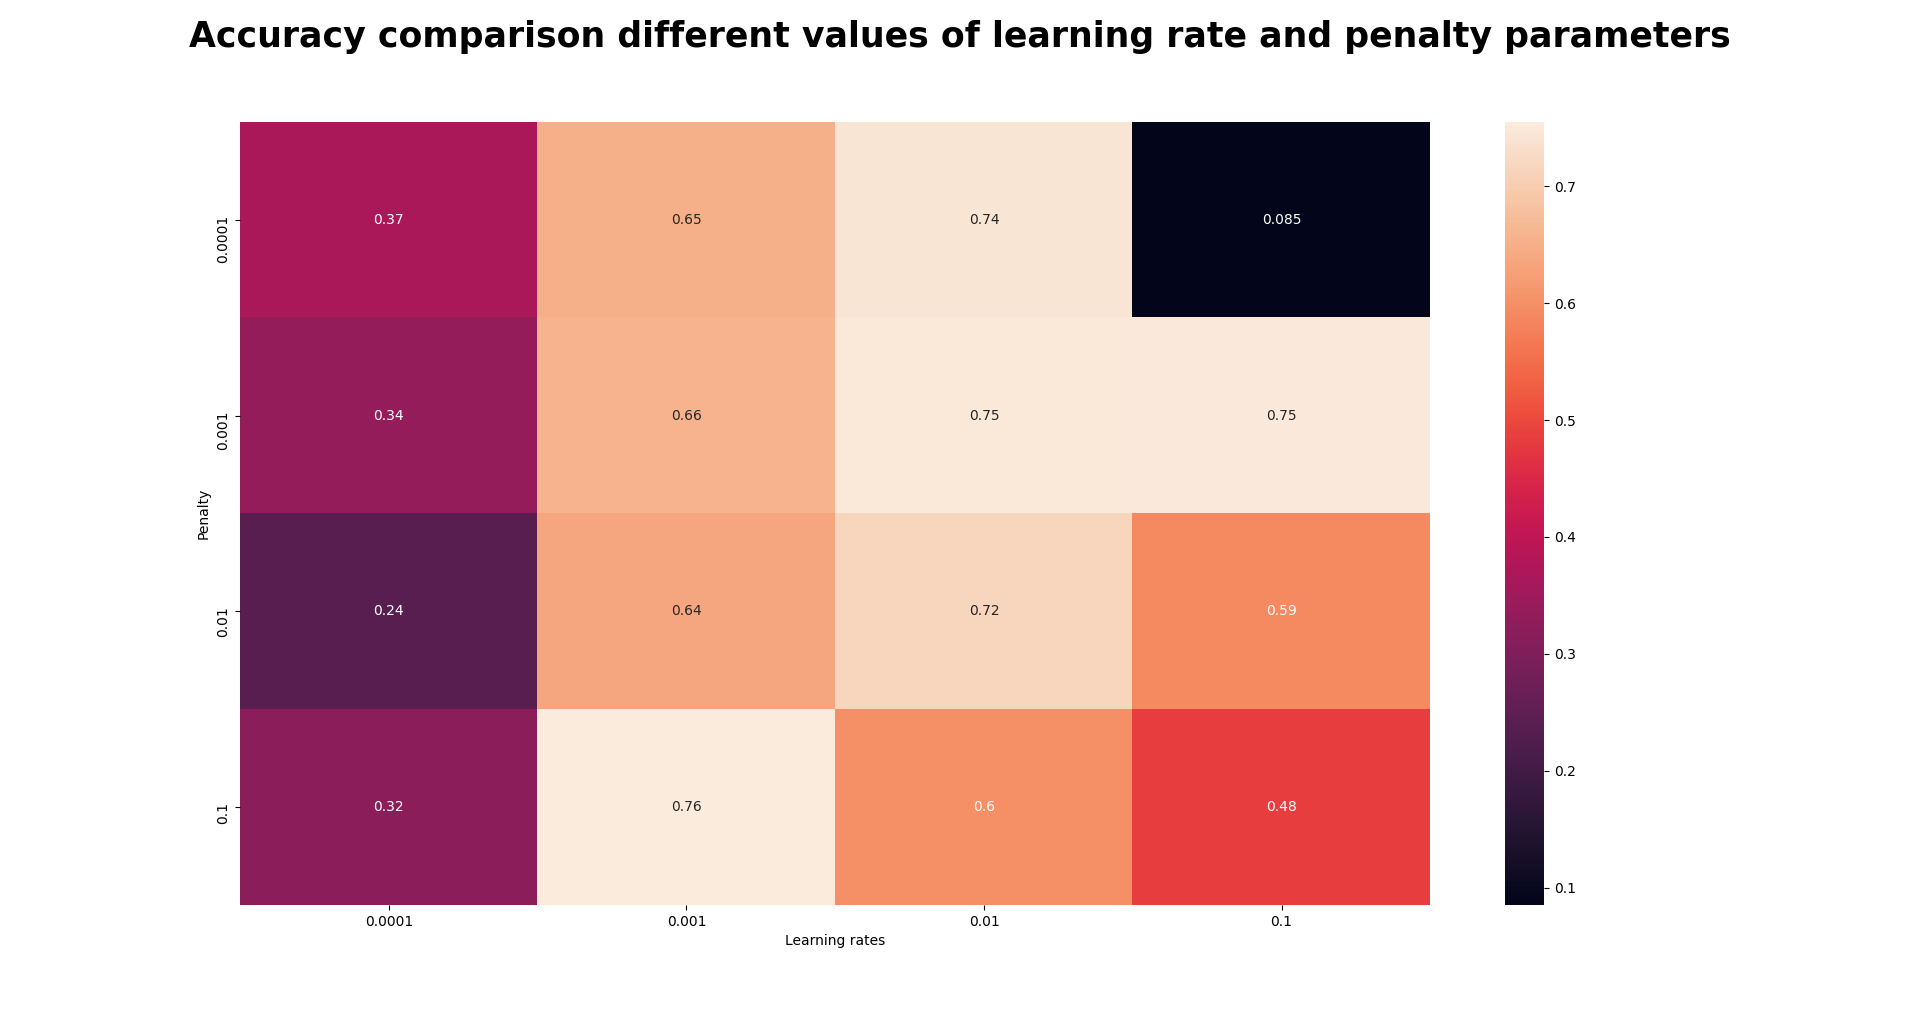
\includegraphics[width = 1\linewidth]{C:/Users/Sander/Documents/GitHub/FYS-STK4155/Project2/Project2/Report/Figures/finalAcc4.PNG}
\caption{\label{fig:finalAcc4} Accuracy as function of both learning rate and penalty for my own implementation.}
\end{figure}

\begin{figure}[H]
\centering
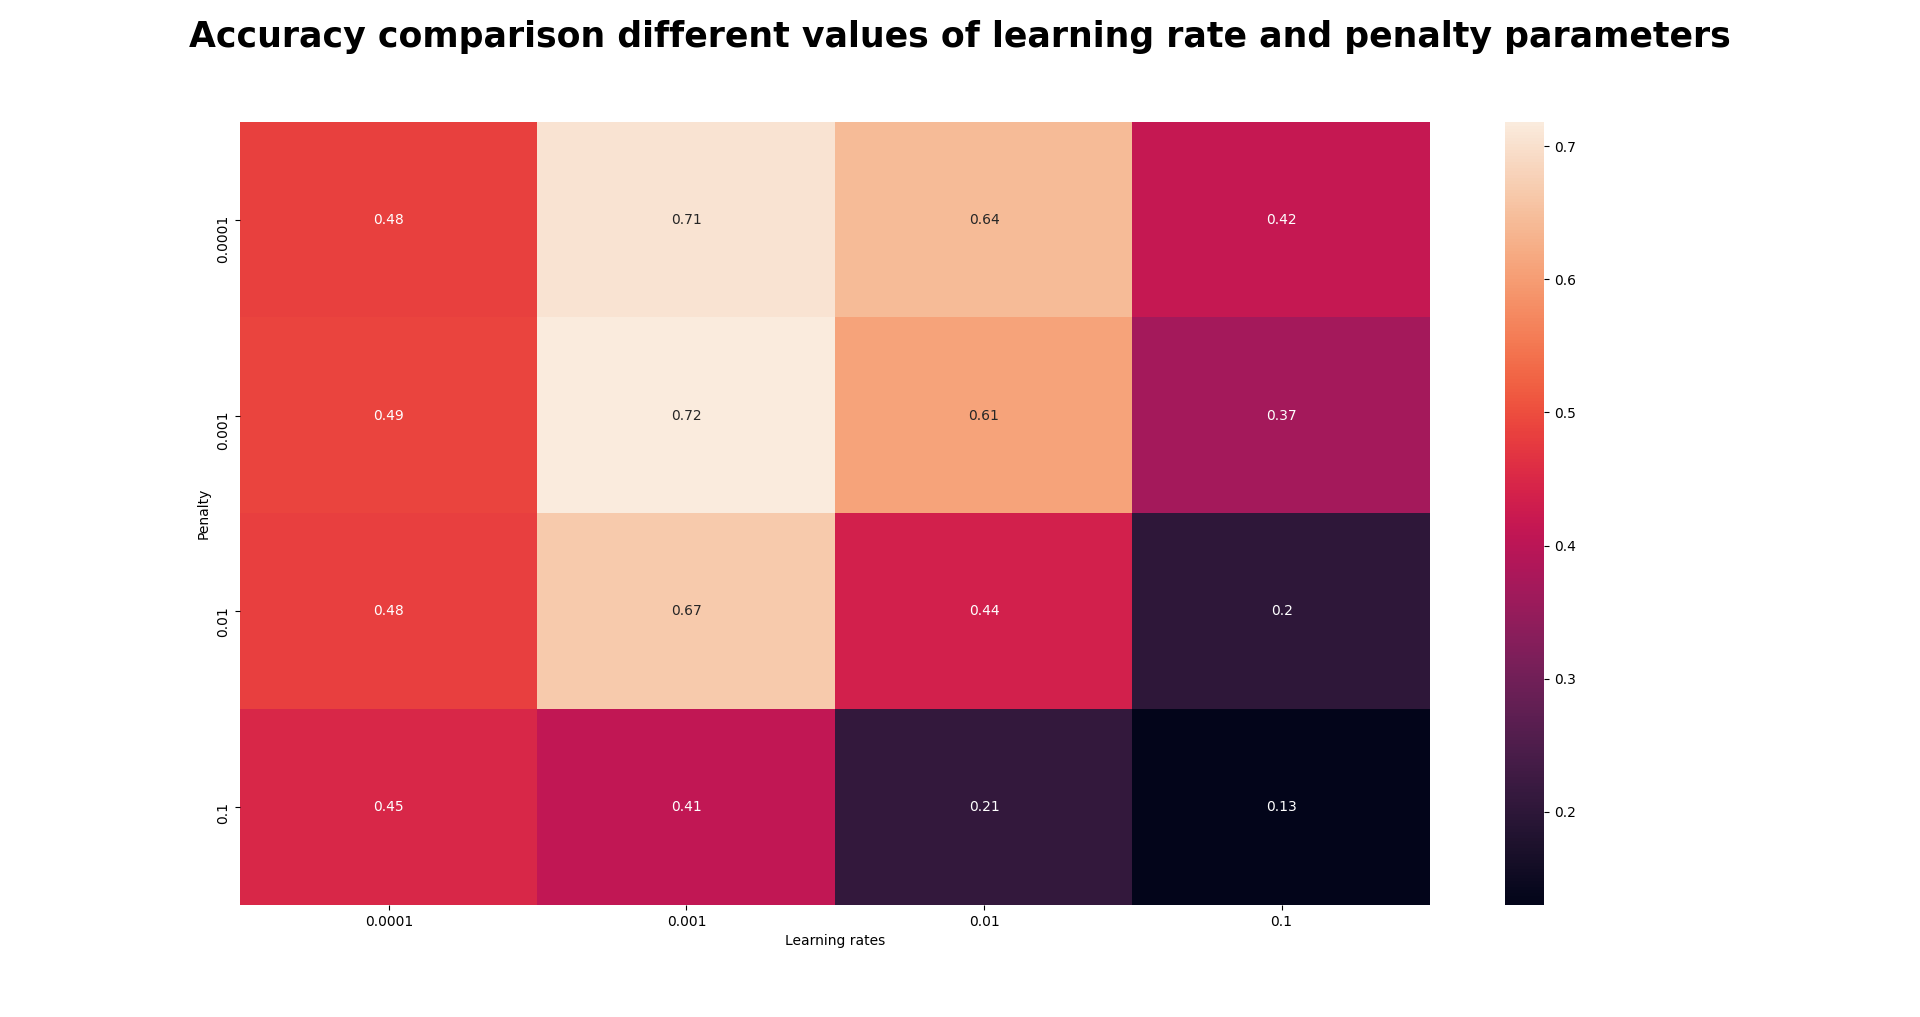
\includegraphics[width = 1\linewidth]{C:/Users/Sander/Documents/GitHub/FYS-STK4155/Project2/Project2/Report/Figures/finalAcc5.PNG}
\caption{\label{fig:finalAcc5} Accuracy as function of both learning rate and penalty for the Scikit implementation.}
\end{figure}

\noindent One can observe from figure \ref{fig:finalAcc4} that the highest accuracy is obtained using by using a penalty of $0.1$ and a learning rate of $0.001$. This is confirmed by looking at the corresponding black line in figure \ref{fig:finalAcc3}. However, one can also observe that there are multiple other good configuration such as a penalty of $0.001$ and a learning rate of $0.01$. This configuration basically yields the same accuracy and it can be observed from the corresponding green line in figure \ref{fig:finalAcc3} that these parameters are good option.
\\
The heatmap for the Scikit implementation seems to be more sensitive to the learning rate and penalty, as the accuracy varies more as seen in figure \ref{fig:finalAcc5}. However, high accuracies of $0.72$ can be obtained with a penalty of either $0.001$ or $0.0001$ and a learning rate of $0.001$. These values corresponds well to what is observed in figure \ref{fig:finalAcc3}.

\newpage

\begin{center}
\Large{\textbf{Exercise f): Evaluation of regression and classification algorithms}}
\end{center}

\begin{center}
\large{\textbf{Comparison between SGD regression and neural network regression of the Franke function}}
\end{center}

\noindent We first aim to compare the OLS equivalent implementations for the SGD regression from exercise 1a) to the OLS equivalent neural network implementation in exercise 1b). Figures \ref{fig:MSEvsEPOCHbatchOLS_sch} and \ref{fig:MSEvsEPOCHlaernOLS} shows that decreasing the batch size and increasing the learning rate yielded lower MSE for the SGD model. Not only that, decreasing the batch size made the SGD algorithm avoid getting "stuck" in a local minimum, which could ruin the MSE totally. However, figure \ref{fig:MSEvsEPOCHbatchOLS_sch} alos shows that decreasing the batch size to a certain point, around 10 in this case, would only yield marginally better results. Increasing the number of epoch iterations would even out some of the differences with models of different batch size and learning rate, but not all. This is evident in figure \ref{fig:MSEvsEPOCHlaernOLS} where the model using a learning rate of $0.0001$ never evens out with the other models, even at a high number of epoch iterations. The MSE of the optimal SGD regression model was about $0.2$.
\\
Much the same can be said for the Ridge equivalent implementation. However, this implementation had a tendency to get "stuck" in local minimum more the the OLS implementation for larger batch sizes, although the opposite is true for smaller batch sizes as seen in figure \ref{fig:MSEvsEPOCHbatchRIDGE}. Since this implementation corresponds to Ridge regression, we can also tune the associated penalty parameter $\lambda$. This parameter was shown in figure \ref{fig:MSEvsEPOCHlambRIDGE} to be of little significance as the MSE was about the same for many different values of $\lambda$. However, when a learning schedule was implemented, the penalty parameter played an essential role in reducing chance of getting "stuck" in a local minimum as seen in figures \ref{fig:MSEvsEPOCHbatchRIDGE_sch} \ref{fig:MSEvsEPOCHlambRIDGE_sch}. 
\\
A neural network regression was implemented and one can observe from figures \ref{fig:MSEvsLrateTOTAL1} and \ref{fig:MSEvsLrateTOTAL2} that utilizing the RELU or leaky RELU implementation yielded great results in terms of MSE and $R^2$, also for the Scikit implementation of RELU. The sigmoid seem to hit some sort of cap where the MSE did not lower using these initial parameters (epoch iterations, batch size etc.). However, when the number of epoch iterations was increased, the sigmoid implementation approached the other implementations more and more as seen in figure \ref{fig:MSEvsLrateTOTAL5} and \ref{fig:MSEvsLrateTOTAL6}. Utilizing a high number of epoch iterations were then used see how the neural network reacted to low batch sizes as seen in figures \ref{fig:MSEvsLrateTOTAL7} and \ref{fig:MSEvsLrateTOTAL8}. One now then observed that the sigmoid again performed worse than the RELU or leaky RELU implementations. Figures \ref{fig:heatmap5}, \ref{fig:heatmap6}, \ref{fig:heatmap7} and \ref{fig:heatmap8} displays how the MSE changes as function of different hidden neuron/layer configurations. It can from these figures be observed that the MSE is relatively high for lower number of hidden neurons/layers, but improves for more hidden neurons and layers. However, the MSE seems to hit a cap where adding more layers and neuron are no longer effective in decreasing the MSE. Additionally, the RELU and leaky RELU experienced overflow within the neural network leading to missing values for some hidden neuron/layer configurations. The sigmoid and Scikit RELU implementations did not experience any overflow.
\\
Much the same can be said for the Ridge equivalent neural network implementation and this implementation yielded similar MSE values to the OLS equivalent implementation. However, the $L_2$ norm associated with Ridge reduced the number of overflow that occurred as seen in figures \ref{fig:heatmap6} and \ref{fig:heatmap8}. For this reason, the Ridge equivalent neural network algorithm is preferred over the OLS equivalent neural network algorithm.
\\
The SGD algorithm was able to push the MSE down to about $10^{-2}$ while the neural network could produce MSE values of about $3 \times 10^{-5}$ when utilizing the RELU or leaky RELU activation function for the hidden layers, as well as the optimal learning rate and $L_2$ penalty. For this reason, I would prefer the neural network, even though it sometimes overflows. The overflow did not occur with the sigmoid activation function which also yielded lower MSEs than the SGD algorithm. However, the SGD algorithm demands fart less computational power, so if an MSE of $10^{-2}$ is good enough for a given data set, then I would prefer to use the SGD. The neural network should be used otherwise.

\begin{center}
\large{\textbf{Comparison between logistic SGD and neural network classification of the MNIST digit data set}}
\end{center}

\noindent The neural network could also be used for classification by changing the activation function for the output layer to the softmax function. The network was then used to attempt prediction of the MNIST hand-written digits and the results were pretty good overall. Different activation function were applied in the hidden layers and the accuracy as function of learning rate can be seen in figure \ref{fig:AccvsLrate}. It is observed that the RELU functions outperforms the sigmoid functions for lower learning rates. This is because the RELU function tends to be unstable at higher learning rates (kilde). However, my sigmoid implementation performs better than the RELU at learning rates above $0.01$ and is then able to accurately predict the hand-written images. From figures \ref{fig:AccvsLrate2} and \ref{fig:AccvsLrate3} it can be observed that the neural network performs great for most hidden neuron/layer configurations. However a chosen few configurations really improves the accuracy to about $0.81$ for the sigmoid implementation and $0.84$ for the RELU implementation. There is little overflow to speak of when the softmax function is applied, resulting in a more robust accuracy (when compared to the MSE form exercise 1b) and 1c)). 
\\
The ridge equivalent implementation behaves quite different to the OLS equivalent implementation discussed above. Figures \ref{fig:AccvsLrate4} and \ref{fig:AccvsLrate5} display how the accuracy behaves as function of learning rates and penalties and it can be observed that the sigmoid implementation is really sensitive to both the learning rate and the penalty, while the RELU implementation only seems to be sensitive to the penalty itself. While the sigmoid implementation steadily increase its accuracy with decreasing learning rate and increasing penalty, the RELU implementation only seems to yield high accuracy for penalties lower than $0.001$. In fact, it appears to be some threshold at this penalty value and the penalty must therefore be chosen below this threshold. Figures \ref{fig:AccvsLrate6} and \ref{fig:AccvsLrate7} shows what happens to the accuracy for the sigmoid and RELU implementations when we vary the number of hidden neurons/layers. One can observe that the sigmoid implementation is really specific in terms of the preferred configurations, as only some configurations yield a high accuracy. The RELU implementation is not that that sensitive. It seems like there are many configurations which yields a high accuracy, but some are optimal. 
\\
We now turn our attention to the logistic SGD case. One can observe from figures \ref{fig:finalAcc2} and \ref{fig:finalAcc3} that my logistic SGD is able to obtain accuracies of just under $0.8$ while the Scikit implementation is able to obtain accuracies just over $0.7$ for both the OLS and Ridge equivalent implementations. One can also observe that there seems to be a optimal penalty of $0.001$ for my own implementation while increasing the penalty in the Scikit implementation only seems to decrease the accuracy. This is analysis is confirmed by figures \ref{fig:finalAcc4} and \ref{fig:finalAcc5} where the optimal penalty for my SGD implementation is $0.001$ and the OLS (penalty of zero) tens to have the highest accuracy in the Scikit implementation.
\\
When comparing the classification neural network to the logistic SGD one finds that the neural network perform much better than the SGD. The difference in accuracy for both optimal models is about $10\%$ in favour of the neural network. The classification neural network did not experience much overflow meaning overflow is not a problem in this case. Therefore, I would prefer using the classification neural network. Having that extra $10\%$ increased accuracy is very significant in many cases. However, the neural network demands much more computational power, but if this is available, I would prefer the classification neural network every time.

\newpage

\begin{center}
\Large{\textbf{Conclusion}}
\end{center}

\noindent a

\newpage

\begin{center}
\Large{\textbf{Future work}}
\end{center}

\noindent a

\newpage

\begin{center}
\Large{\textbf{References}}
\end{center}

\begin{itemize}
  \item a
\end{itemize}

\end{document}
